%\documentclass[11pt,a4paper,twoside]{tesis}
% SI NO PENSAS IMPRIMIRLO EN FORMATO LIBRO PODES USAR

\documentclass[11pt,a4paper]{tesis}
%\setcounter{tocdepth}{3}
\setcounter{secnumdepth}{3}

\usepackage{graphicx}
\usepackage[utf8]{inputenc}
\usepackage[spanish]{babel}
\usepackage{biblatex}
\usepackage{csquotes}
\usepackage{fancyhdr}
\usepackage{amsmath}
\usepackage{amssymb}
\usepackage[lofdepth,lotdepth]{subfig} % para colocar varias imagenes en una misma figura
\usepackage{nameref} % para referenciar y que muestre el titulo de la seccion
\usepackage{lipsum} % para generar texto aleatorio
\usepackage{ulem} % para tachar texto
\usepackage[ruled,vlined]{algorithm2e} % para los algoritmos.
\renewcommand{\listalgorithmcfname}{Índice de algoritmos}
\usepackage{booktabs} % para las tablas.
\usepackage{adjustbox} % para que las tablas no se salgan del margen.
\usepackage{arydshln} % para agregar lineas puntuadas a tablas
\SetKw{Continue}{continue}

\usepackage{titlesec} % para dar estilos a titulos de secciones
\titleformat{\subsubsection}
{\normalfont\normalsize\bfseries}{\thesubsubsection.}{1em}{}

\setlength{\marginparwidth}{2cm}
\setlength{\headheight}{15pt}

\usepackage{todonotes}

\usepackage[left=3cm,right=3cm,bottom=3cm,top=3cm]{geometry}

\usepackage{hyperref}
\hypersetup{
	linktoc=all,
	hidelinks,
}

% Bibliography
\addbibresource{tesis.bib}

% Glossary
\usepackage[acronym]{glossaries}
\makeglossaries
\newglossaryentry{domain-knowledge}{%
	name={domain knowledge},%
	description={valid knowledge used to refer to an area of human endeavour, an autonomous computer activity, or other specialized discipline}}

%batch/ambiente batch
%streaming/ambiente streaming
%framework
%feature
%mineria de datos
%aprendizaje automatico
% inteligencia artificial
% árboles de decisión
%naive bayes
% procesamiento de lenguaje natural
% meka
% weka
%cidetic
% clustering
% python
% java

\newacronym{mll}{MLL}{Clasificación multi-etiquetas}
\newacronym{moa}{MOA}{Massive Online Analysis}
\newacronym{ia}{IA}{Inteligencia Artificial}
\newacronym{ti}{TI}{Tecnología de la Información}
\newacronym{id3}{ID3}{Iterative Dichotomiser 3}
\newacronym{cart}{CART}{Classification and Regression Tree}
\newacronym{br}{BR}{Binary Relevance}
\newacronym{cc}{CC}{Classifier Chains}
\newacronym{lp}{LP}{Label Powerset}
\newacronym{lc}{LC}{Label Combination}
\newacronym{ebr}{EBR}{Ensamble de Binary Relevance}
\newacronym{ecc}{ECC}{Ensamble de Classifier Chains}
\newacronym{ps}{PS}{Pruned Set}
\newacronym{ht}{HT}{Hoeffding Tree}
\newacronym{mlht}{MLHT}{Multi-label Hoeffding Tree }
\newacronym{isoup}{iSoup-Tree}{Incremental Structured Output Prediction Tree}
\newacronym{rtg}{RTG}{Generador de Árbol Aleatorio}
\newacronym{rbf}{RBF}{Generador de Función Radial Base}
\newacronym{vp}{VP}{Verdaderos Positivos}
\newacronym{vn}{VN}{Verdaderos Negativos}
\newacronym{fp}{FP}{Falsos Positivos}
\newacronym{fn}{FN}{Falsos Negativos}
\newacronym{efmp}{EFMP}{Ensamble Fijo por Mayoría Ponderada}
\newacronym{efmp2}{EFMP2}{Ensamble Fijo por Mayoría Ponderada 2}
\newacronym{dwm}{DWM}{Dynamic Weighted Majority}
\newacronym{gooweml}{GOOWE-ML}{GOOWE-ML}
\newacronym{cidetic}{CIDETIC}{Centro de Investigación, Docencia y Extensión en TIC de la Universidad Nacional de Luján}


\newcommand{\comillas}[1]{``#1''}

\begin{document}

%%%% CARATULA
% textidote: ignore begin
\def\titulo{Licenciado }

\def\autor{Juan Cruz Cardona}
\def\tituloTesis{Algoritmos de Clasificación Multi-etiquetas en Ambientes de
	\textit{Streaming} de Datos}
\def\runtitulo{Algoritmos de Clasificación Multi-etiquetas en Ambientes de
	\textit{Streaming} de Datos}
\def\runtitle{Algoritmos de Clasificación Multi-etiquetas en Ambientes de
	\textit{Streaming} de Datos}
\def\director{Santiago Banchero}
\def\fecha{2021}
% textidote: ignore end

% textidote: ignore begin
\newcommand{\HRule}{\rule{\linewidth}{0.2mm}}
%
\thispagestyle{empty}

\begin{center}\leavevmode

\vspace{-2cm}

\begin{tabular}{l}

\includegraphics[width=5cm]{img/logo_unlu}
\end{tabular}

{\large \sc Universidad Nacional de Luján}

\vspace{5.0cm}

{\huge\bf \tituloTesis}

\vspace{2cm}

{\large Tesina de grado presentada para optar al t\'{\i}tulo de\\
\titulo en Sistemas de Informaci\'on}

\vspace{2cm}

{\Large \autor}

\end{center}

\vfill

{\large

{Director: \director}

\vspace{.2cm}

\begin{center}
\fecha
\end{center}
}

\newpage\thispagestyle{empty}

% textidote: ignore end

%%%% ABSTRACTS, AGRADECIMIENTOS Y DEDICATORIA
\frontmatter
\pagestyle{empty}
%\begin{center}
%\large \bf \runtitulo
%\end{center}
%\vspace{1cm}
\chapter*{\runtitulo}

\noindent La clasificación multi-etiquetas es un paradigma de aprendizaje
supervisado que generaliza las técnicas clásicas de clasificación para abordar
problemas en donde cada instancia de una colección se encuentra asociada a
múltiples etiquetas. La mayor parte de los trabajos de investigación han sido
realizados en contextos de aprendizaje por \textit{batch}. Los ambientes de
flujo continuo de datos  (o \textit{streaming}) presentan nuevos desafíos a esta
área debido a las limitaciones de tiempo de respuesta y almacenamiento que
acarrean. En la presente investigación se aplican algoritmos de clasificación
multi-etiquetas a colecciones estructuradas y no estructuradas. Los experimentos
se llevaron a cabo en ambientes simulados de \textit{streaming} de datos para
conocer el impacto que produce este contexto sobre los resultados de la
clasificación y acoplar el modelo a escenarios del mundo real. A su vez, se
partió de estas colecciones de datos para generar instancias sintéticas y así
producir flujos potencialmente infinitos. A este fin se presenta un método de
generación de instancias sintéticas que busca replicar fenómenos particulares de
colecciones multi-etiquetadas. Por último, se diseña una estrategia de ensambles
de algoritmos, \acrshort{efmp}, en búsqueda de una mejora en la calidad de la
tarea de predicción de objetos no observados por el modelo. De esta manera, se
provee a la comunidad de nuevos estudios experimentales sobre algoritmos y
colecciones ya conocidos del área de clasificación multi-etiquetas, de manera
tal de extender el conocimiento sobre su rendimiento bajo escenarios evolutivos
y de naturaleza variable.

\bigskip

\noindent\textbf{Palabras claves:} clasificación, multi-etiquetas, \textit{streaming}, algoritmos, flujos.


%\cleardoublepage
%\chapter*{Agradecimientos}

\noindent En el tiempo que llevó realizar esta tesis he recibido el apoyo y
asistencia de mucha gente y quiero aprovechar este espacio para reconocerlo.

Me gustaría agradecer en primer lugar a mi director, Santiago Banchero, quien
con su conocimiento y experiencia me ha guiado por cada una de las etapas de este
proceso. Su perseverancia y compromiso desde el inicio ha sido esencial para
encauzar este proyecto y ha logrado sacar lo mejor de mí en el proceso.

Además,s agradezco al Centro de Investigación, Docencia y Extensión en TIC de la
Universidad Nacional de Luján (CIDETIC) por proveer los recursos humanos y
computacionales necesarios para este proyecto. No hubiese podido arribar a estos
resultados de no haber sido por el soporte por ellos recibido.

También quiero agradecer especialmente a mi familia, por el sostén emocional a
lo largo de este proceso y por confiar en mí, en las buenas y en las malas.
Gracias a mis padres, a mis hermanas y a mi abuela Lucía.  Finalmente, este
objetivo no se hubiera cumplido sin el apoyo incondicional de mis amigos,
quienes estuvieron junto a mí y supieron entender mis ausencias. Incluso se han
tomado el tiempo de leer los esbozos del escrito, participar en exposiciones o
compartir charlas conmigo, y eso es un privilegio. Por eso gracias Lucas, Luz,
Vicky, Mica, Torne y Alan.
  OPCIONAL: comentar si no se quiere

%\cleardoublepage
%\hfill \textit{A L. C.}
   OPCIONAL: comentar si no se quiere

\cleardoublepage
\tableofcontents
\begingroup
\let\clearpage\relax
\vspace{1cm}
\listoffigures
\vspace{1cm}
\listoftables
\vspace{1cm}
\listofalgocfs
%\vspace{1cm}
%\listoftodos
\endgroup

\mainmatter
\pagestyle{fancy}

%%%% ACA VA EL CONTENIDO DE LA TESIS
\chapter{Introducción}

\section{Fundamentos}

En los últimos años ha habido un aumento considerable de datos de diversa índole
y generados por fuentes heterogéneas. Según los autores
\citeauthor{gantz_extracting_2011}, el volumen total de datos creados y
replicados en el mundo durante el año 2011 supera los 1.8 ZB (zettabytes) y se
ha estimado que duplica cada dos años \cite{gantz_extracting_2011}. Los avances
en el área de tecnología de la información (IT) han contribuido a una continua
producción de datos y expansión del campo digital, tal es el caso para la red
social \textit{Facebook}, la cual recibe cada hora un flujo de 10 millones de
fotos que publican sus usuarios \cite{mayer-schonberger_big_2013}. A estas
grandes colecciones de datos se las conoce como \textit{big data} y acarrean
nuevas oportunidades y desafíos al campo de las ciencias de la computación. En
cuestiones económicas, un análisis a gran escala en búsqueda de tendencias en el
comportamiento de los usuarios o clientes de un sistema puede dar una ventaja
competitiva en el mercado y, en adición, proveer de un servicio valioso a la
comunidad. Potencialmente, la \textit{big data} puede ser una fuente que
proporcione a la comunidad de conocimiento nuevo sobre el mundo en el que
habita, o como ha mencionado \citeauthor{fayyad_advances_1996} en su escrito
sobre el descubrimiento de conocimiento, “Los datos que percibimos de nuestro
ambiente son la evidencia básica que usamos para construir teorías y modelos
sobre el universo en el que vivimos”\footnote{“Data we capture about our
   environment are the basic evidence we use to build theories and models of the
universe we live in” \cite[p. 2]{fayyad_advances_1996}. Traducción propia.}.

Sin embargo, volúmenes masivos de datos tornan obsoletos los tradicionales
métodos manuales de análisis de datos y surge la necesidad de desarrollar
técnicas automatizadas para extraer patrones en los datos y obtener
conocimiento. Con este fin, se han desarrollado técnicas en las áreas de minería
de datos y aprendizaje de máquinas que abordan estas colecciones en búsqueda de
conocimiento válido y útil. Dichas técnicas se han enfocado en el aprendizaje
por \textit{batch} \cite{gama_knowledge_2010}, lo que significa que el algoritmo
dispone de la colección completa, almacenada en disco, y con la cual genera un
modelo a partir de una o múltiples iteraciones sobre todos los datos. No
obstante, el aprendizaje por \textit{batch} trae aparejada una dificultad en su
misma definición: requiere de todos los datos de la colección presentes y
accesibles en todo momento,  lo cual no siempre es posible. Además se suma una
limitante que es clave en el contexto actual de alta disponibilidad de datos:
hoy en día una buena parte de los datos generados proviene de flujos continuos o
‘\textit{streamings}’ de datos \cite{bifet_big_2014}. Estos flujos son
potencialmente ilimitados, arriban de a una instancia por vez, y son analizados
con restricciones altas de tiempo de procesamiento y de memoria.  Tal es el caso
para aplicaciones de sensores, monitoreo de redes y administración de tráfico,
flujo de clics de un usuario en la web, redes sociales, entre otros.  Los
algoritmos de aprendizaje que actúen en este entorno dinámico deben contar con
mecanismos que permitan manejar cambios en la naturaleza o distribución de los
datos, tanto para incorporar datos nuevos, como para descartar los datos
antiguos. Por estas razones, se torna necesario que las aplicaciones basadas en
clasificación en tiempo real adapten sus operaciones de entrenamiento y
predicción para lograr mejores resultados \cite{sousa_multi-label_2018}.

Dentro del área de minería de datos, una de las principales tareas es la de
clasificación, la cual consiste en entrenar un modelo que sea capaz de asignar
una única etiqueta a una instancia desconocida. No obstante, existen problemas
de clasificación en donde múltiples etiquetas son necesarias para caracterizar
una instancia. Por ejemplo, una noticia de diario referida al accidente aéreo
que sufrió el plantel de fútbol del club Chapecoense puede ser clasificado en la
categoría de “Fútbol” tanto como en la de “Tragedias”. Del mismo modo, un video
documental sobre la vida de Borges puede anotarse como “Biografía”, “Literatura”
o incluso “Buenos Aires” si se mostraran imágenes de la ciudad. Este tipo de
problemas es llamado \acrfull{mll} \footnote{Siglas provenientes de su
abreviación en inglés, Multi-label learning} y representa un nuevo paradigma de
aprendizaje automático, con sus propios retos por afrontar y que aún no ha sido
suficientemente explorado en proyectos de investigación. 

Una clasificación multi-etiqueta permite conocer el grado de correlación entre
una instancia de la colección y una o más etiquetas. Esta cualidad significa un
mayor poder de generalización con respecto a la clasificación tradicional de
única etiqueta, ya que puede abarcar esos mismos problemas y otros de mayor
número de etiquetas. Además existen algoritmos que aprovechan la correlación
entre etiquetas para mejorar la eficiencia de la clasificación y la calidad de
la predicción.

El campo de \acrshort{mll} se ha desarrollado considerablemente en los últimos
años pero hasta el momento muchos de estos trabajos se han llevado a cabo en
ambientes estáticos de aprendizaje por \textit{batch}
\cite{read_classifier_2011}. Por lo que se hace necesario encarar nuevos
proyectos que aborden clasificaciones \acrshort{mll} en contextos de
\textit{streaming} de datos. El desafío entonces consiste en crear
clasificadores que sean capaces de manejar un inmenso número de instancias y
adaptarse al cambio, a la vez que estar preparados para hacer tareas de
predicción en cualquier momento, y todo esto en un contexto de altas
restricciones de tiempo de respuesta y memoria.

\section{Clasificación de flujos de datos multi etiquetados} \todo[inline]{Datos
multietiquetados.} \todo[inline]{Aprendizaje incremental ?}
\todo[inline]{Streamings. Caracteristicas esenciales (potencialmente infinita,
limite de espacio en memoria y de tiempo, etc).} \todo[inline]{Caracteristicas
de una colección multietiquetada (densidad, cardinalidad,etc).}


\section{Motivación} 

Ante la necesidad de hacer frente a un contexto global de generación masiva de
datos y a un ritmo cada vez mayor, se hace preciso fortalecer las técnicas de
aprendizaje automático actualmente presentes en el campo. En este escenario ya
no es posible contar con todos los datos almacenados y la idea de generar un
modelo completo para luego evaluarlo en una fase posterior debe ser reemplazada
por una en donde el modelo esté siempre listo para realizar predicciones y al
mismo tiempo ser capaz de re-entrenarse y recalcular las métricas de evaluación
ante cada nueva instancia abordada. Todo esto en un contexto cambiante, de alta
disponibilidad y limitación en el espacio de almacenamiento. Si bien existen
métodos de clasificación para flujos continuos que han dado resultados
satisfactorios, aún es un campo poco abordado y se hace necesario reproducir los
experimentos realizados y fortalecer las técnicas y herramientas actuales para
llevar adelante estudios precisos y pormenorizados.

Por otro lado, si bien existen en el mundo real infinidad de datos multi
etiquetados aún no es posible hallar colecciones disponibles al público que
cuenten con todas las características de un flujo continuo de datos. Uno de los
enfoques abordados es convertir las colecciones existentes en flujos que arriban
a lo largo del tiempo y en cantidades predefinidas. De esta manera los
algoritmos pueden realizar clasificaciones en un ambiente similar al de un
escenario de \textit{streaming}. Sin embargo, estas colecciones tienen un número
limitado de instancias y por lo tanto no cumplen con la condición de ser
teóricamente infinitos. Es entonces aquí donde surgen las técnicas de generación
sintética de instancias, que buscan reproducir la distribución subyacente de los
datos para simular colecciones de datos del mundo real. La contracara de este
enfoque es que, si bien existen técnicas y herramientas para generar datos
etiquetados, buena parte de ellos son solo aplicables para instancias de una
única etiqueta y los que logran generar datos multi etiquetados no han sido lo
suficientemente explorados en el área. Estos son capaces de generar datos
cercanos a los de colecciones del mundo real \cite{read_generating_nodate} y
brindan la posibilidad de realizar estudios certeros de algoritmos de
clasificación \cite{read_scalable_2012}. Pero debe notarse también que si bien
se han obtenido colecciones sintéticas en sí mismas aún no han logrado generar
instancias para una colección en concreto, respetando sus cualidades
particulares y que las distinguen de otras, tales como la co-ocurrencia de
etiquetas, la densidad y cardinalidad de las etiquetas y la relación entre las
etiquetas y sus \textit{features}, por mencionar algunas. De lograr esta
aproximación se podrá realizar estudios sobre el impacto de los algoritmos sobre
flujos de datos de naturaleza distintiva, o en otras palabras, entender en qué
medida un algoritmo es más apropiado que otro para un conjunto de datos en un
determinado contexto. 

\todo[inline]{explicar enfoque de clasificación por ensambles.}





\section{Objetivos} Acá van los objetivos.

\section{Aportes} Acá van los aportes.

\section{Organización del Trabajo} Acá va la descripción de las distintas
secciones del trabajo.

\chapter{Preliminares}

En esta sección se presenta el marco teórico de este trabajo, dando un panorama
general de cada una de las disciplinas abordadas e introduciendo los conceptos
básicos y fundamentales para entender el proyecto. Se comienza con la definición
de la taxonomía del campo de estudio, luego \todo{describir las siguientes
secciones}

\section{Taxonomía del Campo de Estudio}

\begin{figure}
   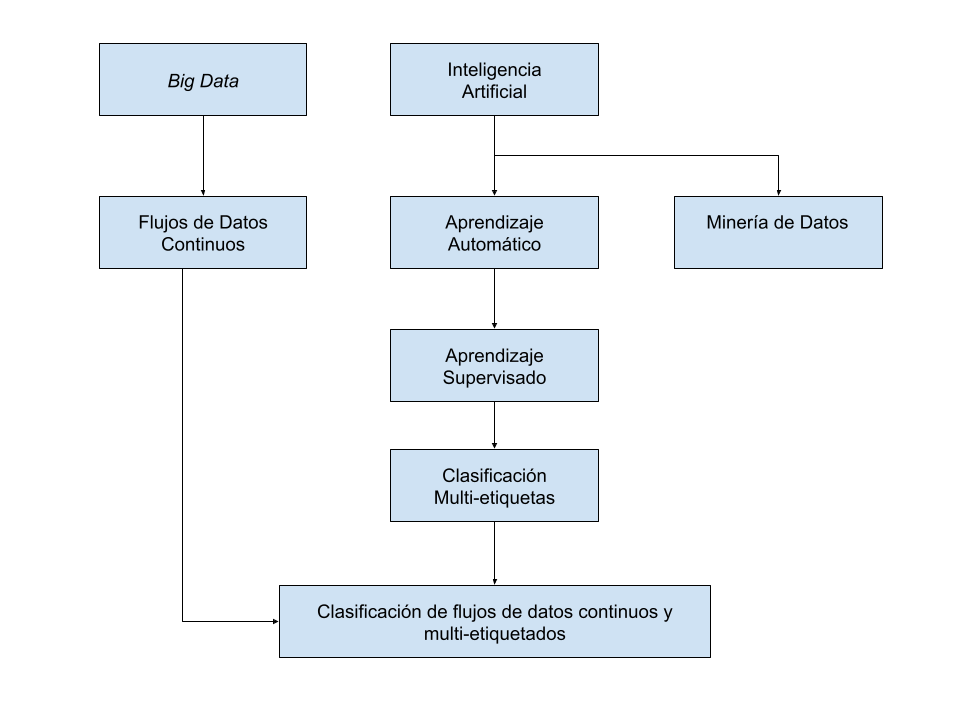
\includegraphics[width=.9\linewidth]{figures/study_field_taxonomy_v2.png}
   \centering
   \caption{Taxonomía del campo de estudio.}
   \label{fig:campo_estudio}
\end{figure}

En pocas palabras, el presente trabajo de investigación se enmarca en las áreas
de \textit{big data} y minería de datos, con aplicación en escenarios de
\textit{streaming} o flujos continuos de datos y abordando clasificaciones
multi-etiquetas. También se aprovechan técnicas del área de procesamiento de
lenguaje natural para tratar corpus de texto libre y extraer \textit{features} o
características representativas de los datos.

La figura \ref{fig:campo_estudio} es un esquema que ilustra la taxonomía del
campo de estudio y la interrelación entre las áreas de investigación
involucradas.

\section{Aprendizaje Automático}

El aprendizaje automático, también conocido por su término en ingles
“\textit{Machine Learning}”, se enmarca dentro del área de la \acrfull{ia} y
estudia cómo las computadoras pueden “aprender” o mejorar su rendimiento
meramente a partir de datos y sin la intervención de un ser humano.  La idea
detrás de esta disciplina es lograr reconocer patrones subyacentes en los datos
y tomar decisiones en base a estos. Por ejemplo, un problema de aprendizaje
automático es el de reconocer dígitos escritos a mano a partir de un conjunto de
ejemplos (ver figura \ref{fig:reconocimiento_digitos}).  Aquí se tienen un
conjunto de imágenes, cada una representando un dígito del 0 al 9, y el objetivo
es construir un modelo que sea capaz de detectar de qué dígito se trata. Otro
ejemplo es el de hallar documentos de texto que son relevantes a una consulta
del usuario. En este caso el modelo recibe un conjunto acotado de términos, los
cuales describen una necesidad de información del usuario, y el modelo debe ser
capaz de retornar los documentos que satisfacen la consulta.  

Estos problemas se suelen categorizar en aprendizaje supervisado o no
supervisado, de acuerdo a si se conoce o no de antemano el concepto o etiqueta
que define a los datos. Se desarrollará más sobre este punto en las próximas
secciones. De entre los problemas de aprendizaje supervisado se destaca aquí el
de clasificación, el cual será descrito a continuación.

\begin{figure}
   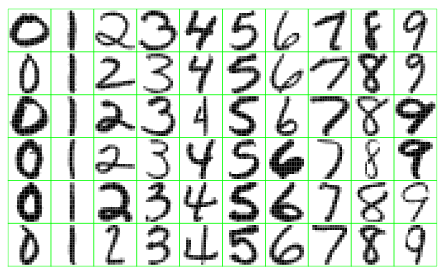
\includegraphics[width=0.66\linewidth]{figures/digits_recognition_v2.png}
   \centering
   \caption{Dígitos escritos a mano. Fuente: \citetitle{hastie_elements_2009}
   (\citeyear{hastie_elements_2009}).}
   \label{fig:reconocimiento_digitos}
\end{figure}

\section{Clasificación}

\subsection{Definición}
\label{clasificacion}

La clasificación es una tarea de minería de datos muy popular que consiste en
hallar modelos que describen la o las clases intrínsecas de los datos. La clase
corresponde a un concepto que representa al dato y es una etiqueta categórica,
es decir, un valor discreto de entre un conjunto de valores previamente
conocidos. Estos modelos, también llamados clasificadores, son capaces de
predecir la clase a la que corresponden datos previamente desconocidos. Por
ejemplo, se puede construir un modelo de clasificación para categorizar nuevos
correos electrónicos  de acuerdo a si se trata de correo basura (también
conocido como "\textit{spam}") o no. Dicho análisis puede ayudar a obtener un
mayor entendimiento de los datos a alto nivel. Las tareas de clasificación han
sido aplicadas en áreas tales como las de aprendizaje automático, reconocimiento
de patrones o estadística. En un principio, buena parte de los algoritmos se
ejecutaban en memoria, con la limitación de espacio de almacenamiento que eso
conlleva. Investigaciones más recientes han desarrollado técnicas para escalar
los algoritmos de tal manera que puedan manejar datos de mayor tamaño, alojados
en memoria, en disco o procesados bajo demanda. Las aplicaciones para este tipo
de tareas son numerosas y entre ellas se encuentran las de detectar fraudes o
realizar diagnósticos médicos, entre otras.

La clasificación de datos consta de dos etapas, una de aprendizaje y otra de
clasificación o predicción. Durante la tarea de aprendizaje se construye el
modelo de clasificación  el cual describe un determinado número de clases o
conceptos. También se conoce esta etapa como la de entrenamiento ya que se
selecciona un subconjunto de los datos, llamado conjunto de entrenamiento, que
consta de instancias o tuplas seleccionadas aleatoriamente y con una o más
etiquetas asociadas. Formalmente, el problema de clasificación puede ser
formulado de la siguiente manera. Se recibe un conjunto etiquetado de
instancias, tupas o ejemplos de la forma $( X, y )$ donde cada tupla es un
vector $X=(x_{1},x_{2},\dots,x_{n})$, siendo cada valor una característica
distintiva, atributo o feature de la instancia. El vector $y$ por su parte toma
un valor de entre $n$ clases diferentes.

Este tipo de tareas se engloban dentro del campo de aprendizaje supervisado ya
que para cada instancia la etiqueta es conocida de antemano, y es aprovechada
para guiar o, siguiendo la metáfora, “supervisar” el aprendizaje del
clasificador. Esta es la diferencia principal contra algoritmos de aprendizaje
no supervisado, en los cuales la etiqueta no es conocida y se deben aplicar
técnicas para salvar esta restricción.

La primera etapa de una clasificación puede ser vista también como el
aprendizaje de una función $y=f(X)$ que pueda predecir la clase $y$ para una
tupla $X$. Por ejemplo, $X$ podría ser un mensaje de correo y la etiqueta $y$ la
decisión de si se trata de un correo basura o no. Desde esta perspectiva
queremos aprender una función que sea capaz de distinguir las clases
subyacentes.  Usualmente, esta asociación es llevada a cabo por algoritmos de
aprendizaje, los cuales internamente usan funciones matemáticas o reglas de
decisión. Algunos ejemplos de este tipo de algoritmos son los árboles de
decisión, \textit{naive} bayes, perceptrón, entre otros.

En la segunda etapa el modelo es usado para clasificar. En primer lugar, se
calcula una métrica de evaluación, tal como la exactitud o \textit{accuracy}.
Durante la etapa de entrenamiento esta estimación puede ser imprecisa, tomando
un valor que tiende a ser “optimista” o que da un valor de exactitud mayor al
rendimiento real. Esto sucede porque el clasificador puede llegar a incorporar
anomalías particulares en el conjunto de datos de entrenamiento. Este fenómeno
es llamado sobreajuste u “\textit{overfit}” y una técnica para reducirlo es
separar de entre los datos un subconjunto de prueba o de \textit{testing} que no
se usa durante el entrenamiento y a partir del cual se realizan predicciones y
se calculan las métricas de evaluación. En este contexto, la tarea de evaluación
es fundamental ya que es la vía a partir de la cual se determina qué algoritmos
o técnicas son más apropiados que otros para un problema en particular. Además
provee la información necesaria para corregir o ajustar los parámetros de los
algoritmos y así obtener modelos más robustos.

En definitiva, ambos pasos se aplican consecutivamente con el objetivo de lograr
hallar un modelo capaz de predecir etiquetas en instancias nuevas y
desconocidas.

\subsection{Algoritmos}
\label{clasificacion_algoritmos}

Como se mencionó en la sección anterior, una de las etapas de clasificación
consiste en generar un modelo capaz de clasificar instancias desconocidas. En
esta etapa se pueden aplicar diversos tipos de algoritmos de acuerdo a la
naturaleza de la tarea en particular que se desea abordar. A continuación se
describen algunos algoritmos para generar modelos y que son particularmente
relevantes para este trabajo de investigación.

\subsubsection{\textit{Naive} Bayes}

\textit{Naive} Bayes es un modelo de clasificación computacionalmente simple
pero cuyo rendimiento es competitivo contra otros modelos más complejos. Se dice
que es un clasificador estadístico ya que se basa en el teorema de Bayes. La
idea es computar una probabilidad para cada una de las clases, basada en los
atributos de la instancia y seleccionar aquella de mayor probabilidad. El
término “\textit{naive}” es el inglés para el término “\textit{ingenuo}” y nace
de la presunción que hace el algoritmo de que los atributos son independientes
entre sí, o condicionalmente independientes. Esta presunción raramente se cumple
en los escenarios donde se aplica pero contribuye a su simplicidad computacional
y a su velocidad durante el entrenamiento.

El teorema de Bayes se define formalmente de la siguiente manera:

\begin{equation}
   P(H \mid X) = \frac{P(X \mid H) P(H)}{P(X)}
\end{equation}

En esta ecuación, el vector $X$ es una tupla definida tal como en la sección
anterior y en términos bayesianos representa la “evidencia”. $P(X)$, por lo
tanto, es la probabilidad de que la tupla contenga los atributos que posee. Por
su parte, $H$ es la hipótesis de que la tupla pertenece a una determinada clase
y $P(H)$ su probabilidad. Esta es conocida como probabilidad “a priori”. De la
misma manera, $P(H|X)$ es la probabilidad de que la hipótesis $H$ sea cierta
bajo la evidencia $X$. A esta se la llama probabilidad “a posteriori” con $H$
condicionada por $X$ y es el valor que se quiere determinar en una tarea de
clasificación.  Finalmente, $P(X|H)$ indica la probabilidad de que la tupla tenga
unos atributos determinados dado que se satisface la hipótesis.

Por su parte, la fórmula de \textit{Naive} Bayes es similar:

\begin{equation}
   P(C_{i} \mid X) = P(X \mid C_{i}) P(C_{i})
\end{equation}

Aquí el término $P(X)$ es descartado ya que se asume constante para todas las
clases. La hipótesis $H$ es representada como $C_{i}$ que es un valor de la
tupla $C=(C_{1},C_{2},\dots,C_{m})$, donde $m$ es el número de clases. La
presunción “ingenua” es aplicada para el cálculo del término $P(X \mid C_{i})$
gracias a lo cual se puede definir de la siguiente manera:

\begin{equation} 
   P(X \mid C_{i}) = \prod\limits_{k=1}^n{P(x_{k} \mid C_{i})} =
   P(x_{1} \mid C_{i}) \times 
   P(x_{2} \mid C_{i}) \times \dots, \times 
   P(x_{n} \mid C_{i})   
\end{equation}

Finalmente, el modelo seleccionará la clase que maximice el valor de
probabilidad.  

Como se ha dicho anteriormente, la simplicidad, velocidad computacional y su
competitividad en métricas de exactitud hacen de \textit{Naive} Bayes un
algoritmo destacado en el campo de aprendizaje automático
\cite{wickramasinghe_naive_2020} y ha sido aplicado para problemas diversos,
tales como el de hallar errores en programas de computación
\cite{arar_feature_2017}, predecir enfermedades del corazón
\cite{dulhare_prediction_2018} o detectar ataques en una red de computadoras
\cite{kalutarage_detecting_2015}.


\subsubsection{Árboles de Decisión}

Los árboles de decisión son un modelo de clasificación que se destaca por ser de
fácil interpretación e intuitivo para el ser humano. De hecho, se puede generar
una representación gráfica del árbol generado para asistir a la comprensión del
del modelo y de cómo se comporta durante una predicción. En cuanto a su
estructura, un árbol de decisión contiene nodos, cada uno representando un
atributo de la colección. Estos nodos se conectan con otros nodos a partir de
enlaces o “ramas” que representan un valor o un rango de valores de ese
atributo. Los nodos de menor jerarquía son llamados “hojas” y contienen la clase
de la predicción, y el nodo de mayor jerarquía es llamado “raíz”. Al momento de
predecir una instancia nueva, la clasificación se realiza de la siguiente
manera:  se toma la instancia nueva, la cual no tiene una etiqueta asociada, y
los valores de sus atributos son comparados contra los del árbol, luego se traza
un camino desde el nodo raíz hasta la hoja que contiene una clase y dicha clase
es la predicción resultante. 

Los árboles de decisión se generan a partir de un algoritmo de inducción.
Existen varios de estos algoritmos pero todos son variantes que han sido
diseñadas bajo un misma principio: construir  el árbol de una manera
“voraz”\footnote{Se le llama voraz o \textit{greedy} a un algoritmo que busca
   hallar la opción óptima en cada paso y, de esta manera, alcanzar la solución
   general óptima para resolver un problema.  Esto lo diferencia de algoritmos
   como los de \textit{backtracking}, los cuales exploran distintas
posibilidades y pueden volver al inicio en búsqueda de una mejor solución},
comenzando desde el nodo raíz (conocido como enfoque \textit{top-down}) y
eligiendo en cada paso el atributo más informativo o que maximice alguna medida
de ganancia de información. 

Algunos de estos algoritmos son:

\begin{description} 

   \item[\acrshort{id3}] Son las siglas de \textit{\acrlong{id3}} y fue
      desarrollado en 1986 por Ross Quinlan. Consiste en crear un árbol de
      múltiples vías, buscando para cada nodo el atributo categórico que lance
      la mayor ganancia de información para las clases categóricas. Los árboles
      crecen en un tamaño máximo y luego se realiza el paso de poda para mejorar
      el poder de generalización del modelo sobre datos desconocidos.

   \item[C4.5] Es la evolución del algoritmo \acrshort{id3}. La principal mejora
      con respecto a su predecesor es que elimina la restricción de que los
      atributos deban ser categóricos. Esto lo consigue particionando el valor
      continuo en rangos o en un conjunto de intervalos discretos. C4.5
      convierte el árbol entrenado en conjuntos de reglas de decisión. 

   \item[\acrshort{cart}] Son las siglas de \acrlong{cart} y es un algoritmo muy
      similar al C4.5 pero que soporta clases numéricas, lo cual permite
      resolver problemas de regresión. 

\end{description}

Una tarea fundamental en la generación de un árbol es definir un criterio de
división para seleccionar el mejor atributo en cada paso. Existen diversas
técnicas para abordarla, una de ellas es la de “Ganancia de Información”, usada
por el algoritmo \acrshort{id3}. La Ganancia de información busca seleccionar el
atributo que posee mayor variabilidad o representatividad de los datos y se
sustenta en el cálculo de la entropía o medida de desorden. La idea de fondo es
hallar el atributo que reduzca la entropía esperada. La entropía en el conjunto
de datos $D$ se calcula de la siguiente manera:

\begin{equation}
   Entropia(D) = - \sum_{i=1}^{m} p_{i}\log_{2}(p_{i})
\end{equation}

Aquí $p_{i}$ corresponde a la probabilidad de que una tupla de $D$ corresponda a
la clase $C_{i}$.  

Luego, la ganancia de información es:

\begin{equation}
   Ganancia(A) = Entropia(D) 
   - \sum_{j=1}^{v} \frac{\left\| D_{j} \right\|}{\left\| D \right\|} 
   \times Entropia(D_{j})
\end{equation}

Aquí el atributo $A$ divide al conjunto de datos en $v$ particiones, siendo $v$
los valores posibles que toma $A$. $D_{j}$ es el subconjunto de los datos cuyas
tuplas poseen el valor $v$ del atributo $A$, siendo $\left\|D_{j}\right\|$ su
cardinalidad o número de instancias del subconjunto. Al dividir este término por
la cardinalidad del conjunto de datos, se obtiene un valor que representa el
peso de la partición y es aplicado sobre la entropía esperada.

Una vez obtenidos los valores de ganancia para cada atributo, se selecciona
aquel que maximiza la ganancia y este será el criterio de separación en el nodo.

El algoritmo C4.5 introdujo una mejora en esta técnica llamada “Razón de
Ganancia”. La misma busca disminuir uno de los efectos adversos que provoca la
técnica de ganancia de información, esta es, que tiende a favorecer a atributos
con un mayor número de valores posibles. La razón de ganancia, en primer lugar,
reemplaza la fórmula $Entropia(D)$ por la siguiente:

\begin{equation}
   EntropiaRG_{A}(D) = - \sum_{j=1}^{v} \frac{\left\| D_{j} \right\|}{\left\| D \right\|} 
   \times \log_{2}(\frac{\left\| D_{j} \right\|}{\left\| D \right\|})
\end{equation}

A su vez, el nuevo cálculo de la ganancia se formula así:

\begin{equation} \label{eq:gan_c45}
   RazonGanancia(A) = \frac{Ganancia(A)}{EntropiaRG_{A}(D)} 
\end{equation}

Finalmente, el atributo de mayor razón de ganancia es seleccionado.

\todo[inline]{Aplicaciones de árboles de decisión en la literatura}

\todo[inline]{Figura de un árbol}

\todo[inline]{Subsección para sgd?, svm?, perceptrones?}

\subsubsection{Ensambles}

Los ensambles son un conjunto de clasificadores que, al ser combinados, pueden
realizar mejores predicciones que cualquiera de ellos individualmente. En pocas
palabras, el enfoque de ensambles consiste en generar $k$ clasificadores, de un
mismo tipo o no, y entrenarlos con subconjuntos de la colección de entrenamiento
original. Dada una tupla nueva, cada clasificador devuelve su propia predicción,
llamada “voto” y luego el ensamble devuelve la predicción final basada en esos
votos.

La aplicación de ensambles en problemas de clasificación nace de la
imposibilidad de generar un único modelo capaz de generalizar lo suficiente como
para lograr un rendimiento perfecto. Ante la presencia de datos ruidosos,
atípicos o erróneos los clasificadores pueden tender a clasificar mejor para un
subconjunto de datos y no tan bien para otros. Este escenario es aprovechado por
el enfoque de ensambles ya que su éxito tiene correlación con la existencia de
diversidad en la clasificación, esto es, que haya variabilidad entre los
subconjuntos de datos, modelos o hiper-parámetros, entre otros factores. A mayor
esta diversidad, los errores particulares de un ensamble se aíslan y serán
filtrados por la clasificación final. Como resultado se espera una disminución
del error total de la clasificación así como también una mayor exactitud en la
predicción, comparando contra los clasificadores base. Por otro lado, un enfoque
de ensambles abre la posibilidad de distribuir y/o paralelizar el cómputo de la
predicción, pudiendo así mejorar los tiempos de ejecución durante el
entrenamiento.

Existen distintos tipos de ensamble, de acuerdo a su construcción y
arquitectura. A continuación se describen 3 de ellos: los ensambles de tipo
\textit{bagging}, los de tipo \textit{boosting} y los de tipo \textit{stacked}. 

\begin{description} 

   \item[Bagging] Esta es una de las primeras técnicas de ensambles conocidas y
      fue introducida por
      \citeauthor{breiman_bagging_1996}\cite{breiman_bagging_1996}. La misma se
      desarrolla de la siguiente manera: dado un conjunto de entrenamiento $D$
      con $n$  tuplas, \textit{bagging} genera un número $m$ de nuevos conjuntos
      de datos de entrenamiento, cada uno con $n$ tuplas. Para esto se toman
      tuplas del conjunto original de manera aleatoria y con reemplazo, es decir
      que puede haber tuplas repetidas y otras que no están incluidas en el
      nuevo conjunto.  Luego a partir de cada conjunto nuevo, se entrena un
      clasificador $M_{i}$. Cada clasificador puede ser del mismos tipo ya que
      la diversidad está dada por los datos. En la etapa de clasificación, cada
      modelo $M_{i}$ genera una predicción que cuenta como un voto. El ensamble
      cuenta los votos y elige la clase con mayor cantidad de votos, siendo esta
      la decisión final del ensamble.


   \item[Boosting] En la técnica de \textit{boosting} se asigna un peso a cada
      tupla de entrenamiento y se generan un conjunto de clasificadores, uno
      luego del siguiente. A diferencia del método de \textit{bagging},
      \textit{boosting} trabaja siempre sobre el mismo conjunto de datos y la
      variabilidad está dada por los pesos que son asignados. El proceso es el
      siguiente: para el primer modelo de clasificación, $M_{i}$, los pesos son
      inicializados en un mismo valor para todas las tuplas. Una vez que se
      entrena este modelo, los pesos son actualizados de tal manera que el
      siguiente clasificador $M_{i} + 1$ trate de manera particular a las tuplas
      mal clasificadas por Mi, de tal manera de llegar a una clasificación
      correcta.  El clasificador final combina los votos de cada clasificador
      individual , donde el peso del voto de cada clasificador es una función de
      su exactitud. 


   \item[Stacking] Stacking es una técnica desarrollada por
      \citeauthor{wolpert_stacked_1992}\cite{wolpert_stacked_1992} y consiste en
      entrenar un nuevo clasificador de acuerdo a las predicciones realizadas
      por otros modelos, tomando la salida de estos modelos como entrada, de tal
      manera de lograr hallar una combinación que produzca una mejor predicción.
      Este tipo de ensambles puede ser visto como un conjunto de capas. La
      primera capa consta de un ensamble de clasificadores que aprenden a partir
      de los datos de entrenamiento. Esta capa no necesariamente usa
      clasificadores del mismo tipo, mismos hiper-parámetros o particiones de la
      colección iguales, quedando estos detalles a cargo de quien diseña esta
      capa. La siguiente capa es el clasificador individual, o
      meta-clasificador, que se alimenta de las salidas de los clasificadores de
      la capa inferior y realiza el aprendizaje a partir de las clases
      producidas por estas salidas y las clases reales.

\end{description}

Una de las tareas a tener en cuenta durante el entrenamiento de un ensamble es
la de combinar las salidas de cada modelo en una salida final. La estrategia más
común y simple es la de mayoría de voto, aplicada por los métodos de
\textit{bagging}, pero existen múltiples y no necesariamente un ensamble de tipo
\textit{bagging} debe aplicar esta estrategia. Por ejemplo, algunos
clasificadores pueden decidir producir una salida sólo en el caso de que más de
la mitad de ellos coincidan, o incluso ser más restrictivos y obligar a que la
coincidencia sea total. El enfoque de \textit{boosting} por su parte, pondera al
voto de acuerdo a los pesos que calcula, dando predominio a determinadas
instancias.  También se suele dar un mayor peso a determinados clasificadores
por sobre otros. Este tipo de métodos se los denomina “mayoría de voto
ponderada” y pueden llevar a un rendimiento superior.

\todo[inline]{Aplicaciones de ensambles en la literatura}

\todo[inline]{Figura de ensamble}

\section{Clasificación Multi-etiquetas}

A diferencia del aprendizaje automático tradicional, que usa datos de etiqueta
única para representar objetos del mundo real, cada instancia en el aprendizaje
multi-etiquetas representa un único objeto pero puede contener más de una
etiqueta. Por consiguiente, la tarea de clasificación consiste hallar una
función que logre asignar a cada objeto, nuevo y desconocido, el conjunto de
etiquetas que lo caracteriza.

En este apartado se da una definición formal, se detallan las características de
un conjunto de datos multi-etiquetados y se  describen algunos métodos
tradicionales de clasificación multi-etiquetas junto con sus ventajas,
desventajas, aplicaciones y motivaciones.

\subsection{Definición Formal y Métricas}

Asumiendo que $X=\mathbb{R}^{d}$ denota el espacio de instancias $d$
dimensional, y que $Y = \{y_{1}, y_{2}, \dots, y_{q}\}$ denota el espacio de
etiquetas con $q$ etiquetas posibles, la tarea de clasificación multi-etiquetas
consiste en entrenar un conjunto $D = \{(x_{i}, Y_{i}) \mid 1 \leq i \leq m\}$
para hallar una función $h$ tal que $h: X \rightarrow 2^y$. A su vez, $X_{i}$ es
un vector de atributos $d$ dimensional definido como $(x_{i1}, x_{i2}, \dots,
x_{id})$. $Y_{i}$, por su parte, es el conjunto de etiquetas sociadas a la
instancia $X_{i}$. Luego, para cada instancia desconocida $X \rightarrow X$ el
clasificador $h$ predice $h(x) \subseteq Y$ que representa el conjunto de
etiquetas hallado para $x$.

A su vez, se definen un conjunto de métricas que describen el grado de
multi-etiquetado que tiene un conjunto de datos dado, o en otras palabras, hasta
qué punto cada ejemplo posee más de una etiqueta. Algunas de ellas son: 

\begin{description}
   \item{Cardinalidad de etiquetas}: Es el promedio de etiquetas por instancia
      del conjunto de datos. Se define como: 
      \begin{equation}
         CardE(D) = \frac{1}{m} \sum_{i=1}^{m} \left\|Y_{i}\right\|
      \end{equation}
      Por lo tanto, a mayor el valor de cardinalidad, mayor es el número de
      etiquetas de una instancia. Por ejemplo, si $CardE = 1$, entonces la
      mayoría de ejemplos tiene una única etiqueta y, por consiguiente, se puede
      decir que la colección tiene un grado bajo de multi-etiquetado.  
   \item{Densidad de etiquetas}: Es la cardinalidad de etiquetas normalizada al
      número total de etiquetas de $D$ y se define como:
      \begin{equation}
         DenE(D) = \frac{CardE(D)}{\left\|Y\right\|}
      \end{equation}
      Así pues, un valor alto de densidad significaría que cada instancia puede
      ser una buena representación de las etiquetas del conjunto. De la misma
      manera, un valor bajo suele implicar dispersión, esto es, que la mayoría
      de las instancias tienen un subconjunto acotado de las etiquetas. 
   \item{Diversidad de etiquetas}: Es el número de conjuntos de etiquetas
      unívocos que aparecen en instancias de $D$. Se define como:
      \begin{equation}
         DivE(D) = \left\|\{Y \mid \exists x: (x, Y) \in D\}\right\|
      \end{equation}
      Aquí la interpretación es que, a mayor el valor de diversidad, menor es la
      constancia con la que las etiquetas aparecen en las instancias. De manera
      similar a la cardinalidad, el valor de diversidad también puede
      normalizarse por el número de instancias del conjunto de datos: 
      \begin{equation}
         DivEProm(D) = \frac{DivE(D)}{\left\|D\right\|}
      \end{equation}
\end{description}

\subsection{Algoritmos}

Como se había anticipado en la sección \ref{intro_mll}, la tarea de aprendizaje
sobre datos multi-etiquetados puede ser encarada siguiendo dos grandes enfoques,
llamados “Transformación del Problema” y “Adaptación del Algoritmo”. A
continuación se describen ambos enfoques y algunos de sus algoritmos más
representativos.

\subsubsection{Transformación del Problema} 

Esta categoría engloba al conjunto de algoritmos que abordan el problema de
clasificación multi-etiquetas transformándolo en múltiples problemas de
clasificación de única etiqueta, lo cual permite aplicar algoritmos de
clasificación convencionales. Tres de estos métodos son particularmente
relevantes para este trabajo: “\acrfull{br}”, “\acrfull{cc}” y “\acrfull{lp}”.

\paragraph{\acrfull{br}}

El algoritmo de Relevancia Binaria, conocido como \textit{\acrlong{br}} en la
literatura, es un enfoque que consiste en descomponer la tarea de clasificación
\acrshort{mll} en $\left\|q\right\|$ clasificadores binarios, independientes y
de etiqueta única.  A partir de esta transformación se puede seleccionar
cualquier algoritmo de clasificación como clasificador base del problema (ver
los algoritmos presentados en la sección \ref{clasificacion_algoritmos}).  Cada
clasificador binario $g_{j}$ es entrenado con todas las instancias de la
colección pero incluyendo solo la etiqueta $j$, la cual se activa o desactiva de
acuerdo a si es relevante a la instancia. Luego la predicción de una instancia
desconocida se realiza combinando las salidas de cada clasificador individual,
esto es: 

\begin{equation}
   Y = {y_{j} \mid g_{j}(x) > 0, 1 \leq j \leq q}
\end{equation}
 
Llegado el caso en que ninguno de los clasificadores retornen etiquetas activas,
el conjunto $Y$ será vacío.

Este enfoque se dice que es de primer orden (ver sección \ref{estrategias_mll})
y no tiene en cuenta la correlación o interdependencias entre etiquetas. Este es
uno de los principales inconvenientes de este algoritmo ya que, en este tipo de
problemas de \acrshort{mll}, es usual hallar que determinadas etiquetas se
activan en conjunto con mayor probabilidad. Pese a ello, \acrshort{br} es un
enfoque muy utilizado \cite{zhang_review_2014} ya que es simple de implementar,
intuitivo y computacionalmente poco costoso en comparación con algoritmos que sí
tienen en cuenta la relación entre etiquetas.  

\paragraph{\acrfull{cc}}

Las cadenas de clasificadores o \textit{\acrlong{cc}}
\cite{read_classifier_2011} es una técnica que convierte el problema de
\acrshort{mll} en una ”cadena” de problemas de clasificación binaria, tal que el
siguiente clasificador de la cadena posee las predicciones de los anteriores. En
principio, la división del conjunto de datos es similar a la que se hace en el
enfoque anterior, designando un clasificador por cada etiqueta. Durante el
entrenamiento el clasificador inicial, seleccionado aleatoriamente, usa de
entrada los atributos originales, tal como el clasificador \acrshort{br}. Luego
la salida de este clasificador es añadida al espacio de atributos como un
atributo más de cada instancia, para que posteriormente, estos atributos sean la
entrada del siguiente clasificador, el cual también es seleccionado al azar.
proceso es repetido hasta completar todos los clasificadores.  Como se ve se
produce un ”encadenamiento” de clasificadores que no es accidental y tiene como
fin conservar la dependencia entre etiquetas, ya que cada clasificador logra
capturar la correlación entre las etiquetas de los anteriores clasificadores. 

Cabe notar que en esta técnica cobra especial importancia el ordenamiento de los
clasificadores ya que este orden tiene un impacto directo sobre el resultado de
la predicción. En otras palabras, si el ordenamiento de clasificadores se
modifica, el modelo final otorgará resultados diferentes. Para salvar esta
dificultad se han propuesto modelos como el de \acrfull{ecc}. El mismo genera un
conjunto de modelos de \acrshort{cc} con distintos ordenamientos y entrenados
con diversos subconjuntos de datos, generados con reemplazo o no. Durante la
predicción, cada cadena produce un conjunto de etiquetas, que son los votos, y
la salida final será computada por un algoritmo que combine cada salida
individual.
 
\paragraph{\acrfull{lp}}

El conjunto de potencias de etiquetas o \textit{\acrlong{lp}}
\cite{tsoumakas_random_2011} es una técnica que se encarga de transformar el
problema de \acrshort{mll} en uno de clasificación multi-clase, de tal manera de
poder abordarlo con algoritmos de este tipo. La clasificación multi-clase es un
enfoque usado para tratar con ejemplos en donde la etiqueta es única pero cuenta
con más de dos clases. Un ejemplo de este tipo de problemas es el de análisis de
sentimiento de texto, en donde las clases pueden ser “positivo”, “negativo” y
“neutral”. 

En \acrshort{lp} cada etiqueta indica el subconjunto de etiquetas de
la instancia. Esto es beneficioso en cuanto a que se logra preservar la
dependencia entre etiquetas. Sin embargo, el modelo tiene algunas dificultades.
En primer lugar, el espacio de clases posibles es exponencial y su cantidad de
clases puede llegar a ser de $2^{\left\|L\right\|}$ como máximo. A su vez, pueden
llegar a arribar ejemplos con una combinación de etiquetas que el modelo no
recibió durante el entrenamiento, por lo cual no logra generalizar lo suficiente
y se lo considera un modelo incompleto. A fin de sobrepasar estas complicaciones
se desarrolló la técnica de Conjuntos Podados o \acrfull{ps}. La misma consiste
en preservar para la clasificación aquellos subconjuntos de etiquetas que son
más frecuentes en la colección, y eliminar los demás. Con esto se logra
disminuir considerablemente el espacio de clases y disminuye la complejidad
computacional, tanto durante el entrenamiento como durante la predicción.

\subsubsection{Adaptación del Algoritmo}

Además del enfoque de transformación del problema, otros autores abordan la
clasificación multi-etiquetas a partir de la adaptación de algoritmos clásicos y
bien conocidos. Esta categoría engloba al conjunto de algoritmos que abordan el
problema de \acrshort{mll} mediante la modificación de algoritmos de etiqueta
única para que sean capaces de manejar la nueva naturaleza de los datos en estas
tareas. Las modificaciones que se introducen pueden variar en complejidad según
el algoritmo tratado y las características de la colección.  Se han adaptado una
diversa cantidad de algoritmos incluyendo aquellos basados en redes neuronales,
árboles, métodos probabilísticos, entre otros \cite{herrera_multilabel_2016}.
Por mencionar algunos ejemplos, \citeauthor{gargiulo_deep_2018} usan redes
neuronales profundas para clasificar documentos de texto libre y comparan su
funcionamiento variando el número de etiquetas y aprovechando su estructura
jerárquica \cite{gargiulo_deep_2018}. Asimismo,
\citeauthor{tanaka_multi-label_2015} agregan al algoritmo de \acrshort{br} la
capacidad de capturar relaciones entre etiquetas a través del uso de árboles de
decisión y lo aplican en el área de la genómica \cite{tanaka_multi-label_2015}.

En lo que confiere a ambientes de flujos continuos de datos una de las técnicas
más populares en la literatura es la de Árbol de Hoeffding o
\textit{\acrfull{ht}} \cite{domingos_mining_2002}. A diferencia de los
algoritmos convencionales de árboles de decisión, \acrlong{ht} aborda los datos
de manera incremental. Así pues, en lugar de realizar decisiones de corte de
acuerdo a los datos previamente almacenados, \acrshort{ht} espera a tener una
cantidad suficiente de instancias para realizar el corte, con un cierto grado de
confianza. Esto significa que ya no es necesario guardar todos los datos de la
colección y que mantener una serie de estadísticas es suficiente para realizar
la clasificación. Otra de las propiedades a destacar de este método es que en
teoría se puede entrenar un árbol cuyo rendimiento se aproxime al generado en un
ambiente de \textit{batch}, con la suficiente cantidad de datos
\cite{bifet_machine_2018}. 

A partir de esto, y buscando sacar provecho de las ventajas mencionadas,
\citeauthor{read_scalable_2012} decidieron adaptar este algoritmo a problemas de
multi-etiquetas y desarrollaron el algoritmo llamado Árbol de Hoeffding
Multi-etiquetado o \textit{\acrfull{mlht}} \cite{read_scalable_2012}. Esto lo
consiguen a partir de rediseñar la fórmula de ganancia de información (ver
fórmula \ref{eq:gan_c45}) de tal manera de reflejar el impacto de todas las
clases a las cuales el ejemplo no pertenece. Desde que fue introducido en el año
\citeyear{read_scalable_2012}, \acrshort{mlht} ha sido usado como modelo de
comparación en reiteradas oportunidades \cite{sousa_multi-label_2018} y es uno
de los métodos más populares para atacar problemas de \acrshort{mll} en
ambientes de flujo continuo de datos.

Otro algoritmo muy popular para abordar este tipo de problemas y basado en
árboles de decisión incrementales es el llamado \acrshort{isoup} (siglas del
inglés \textit{\acrlong{isoup}}) \cite{osojnik_multi-label_2017}. El mismo fue
desarrollado inicialmente para hacer regresión de múltiples objetivos y luego
fue adaptado a tareas de \acrshort{mll}. Una de las novedades que introduce es
el uso de un perceptrón adaptativo en las hojas del árbol, lo cual le da la
versatilidad de poder trabajar tanto con problemas de clasificación como de
regresión.

\section{Clasificación de Flujos Continuos de Datos}

\section{Evaluación y Métricas}


\chapter{Metodología}

Conforme a los objetivos planteados en la sección~\ref{intro_objetivos} se
presentan las colecciones y algoritmos que serán evaluados junto con el
escenario de flujos continuos diseñado a este fin.

Se seleccionan tres colecciones de datos de multi-etiquetas que han sido puntos
de referencia en otros trabajos de investigación. Cada uno de ellos es
transformado en un flujo continuo de datos que cumple con las características
presentadas en la sección~\ref{stream_caracteristicas}. A su vez, se generan
instancias sintéticas que sean fieles a las cualidades subyacentes de los datos
originales.  Para ello, se ha diseñado un algoritmo basado en la implementación
de \citeauthor{read_multi-label_2008} \cite{read_multi-label_2008} pero que hace
uso de la matriz de probabilidades condicionales entre pares de etiqueta para
respetar sus interdependencias.

La etapa de entrenamiento se lleva a cabo con algoritmos de clasificación
multi-etiquetas que han sido adaptados a ambientes de flujos continuos para
hacer frente a las cualidades incrementales inherentes a este contexto. Se
seleccionan algoritmos de la familia de \comillas{Transformación del problema} y
\comillas{Adaptación del algoritmo} \todo{por el momento no se experimentó con
	algoritmos AA en Python}, junto con soluciones de ensamble, a fines explorativos
y para extender el conocimiento sobre sus fortalezas y debilidades. Los
experimentos se realizan con algoritmos implementados en el lenguaje de
programación Python.  Aquellos que no soportan datos de múltiples etiquetas han
sido acondicionados a ese fin de acuerdo al diseño especificado en la literatura
y consultando las respectivas implementaciones en otros lenguajes de
programación, de hallarse estas disponibles al público.

De manera complementaria, se diseña una solución de ensambles llamada
\acrfull{efmp} \todo{nombre tentativo}, basada en las implementaciones
existentes. La misma usa como clasificadores base tres algoritmos de
\acrshort{mll} diferentes, que se mantienen fijos durante todo el entrenamiento.
Además, el ensamble mantiene una ponderación de cada clasificador de acuerdo a
su rendimiento, penalizando por cada etiqueta mal clasificada, y la combinación
de los votos se lleva a cabo por mayoría de voto ponderada. La implementación se
basa en la presentada
por~\citeauthor{kolter_dynamic_2007}~\cite{kolter_dynamic_2007}, quienes también
ponderan los clasificadores pero usan un único tipo de clasificador base y no
contemplan problemas de múltiples etiquetas. Los experimentos se realizan con
dos versiones, una de ellas se entrena con todas las instancias del subconjunto
de entrenamientos y la otra tomando muestreos siguiendo la distribución de
\textit{poisson}, tal como se realiza para ensambles del tipo de \textit{Oza
	bagging} \cite{oza_online_2005}.

Para la etapa de evaluación se sigue la estrategia
\comillas{\textit{Prequential}}, descripta en la
sección~\ref{stream_evaluacion}, y se aplican métricas basadas en etiquetas y
ejemplos, se mide la eficiencia de los modelos en términos de velocidad y
espacio de almacenamiento y se analizan los resultados obtenidos.

El marco metodológico de este proyecto se ajusta a los procedimientos efectuados
previamente por otros investigadores de la literatura
\cite{osojnik_multi-label_2017, sousa_multi-label_2018, buyukcakir_novel_2018,
	zheng_survey_2020, read_scalable_2012}. Con ello se busca expandir el
conocimiento empírico de los algoritmos al mismo tiempo que proporcionar nuevos
estudios que sean contrastables con los ya existentes.  Se destaca el trabajo de
\citeauthor{read_scalable_2012} \cite{read_scalable_2012}, quienes analizan
algoritmos multi-etiquetas con flujos reales y sintéticos, pero a diferencia de
este trabajo, generan instancias sintéticas para colecciones nuevas y sin
basarse en colecciones reales específicas. La implementación del generador que
usaron en sus experimentos se encuentra disponible al público
\footnote{\url{shorturl.at/frsHU}} y ha sido el punto de partida para
desarrollar la técnica aquí propuesta.  \citeauthor{buyukcakir_novel_2018}, por
su parte, no generan flujos sintéticos pero conducen experimentos similares en
lo que respecta al análisis de algoritmos, poniendo el foco en modelos de
ensambles.  La implementación de sus experimentos también ha sido liberada al
público~\footnote{\url{https://github.com/abuyukcakir/gooweml}} pero solo para
el lenguaje de programación Java.


\section{Técnicas Propuestas}

En esta sección se describen dos técnicas implementadas para este trabajo: un
generador de instancias sintéticas para flujos continuos de datos y el diseño de
una solución de ensambles para realizar clasificaciones.

\subsection{Generación de Flujos Sintéticos}

El generador presentado es un algoritmo que emplea técnicas probabilísticas para
hallar dependencias entre etiquetas y reproducirlas en las nuevas instancias. La
existencia de interdependencias entre etiquetas ha sido explorada reiteradas
veces en la literatura \cite{tsoumakas_multi-label_2007, read_multi-label_2008}
y se ha demostrado que existen dependencias condicionales e incondicionales,
esto es, etiquetas que dependen entre sí dado uno o más atributos de una
instancia (dependencia condicional), y etiquetas cuya dependencia existe para
todo el conjunto de instancias (dependencia incondicional). Estas dos cualidades
son directamente extraídas de las colecciones reales y a partir de ellas se
genera el espacio de atributos y etiquetas que, al fusionarse, constituyen la
instancia sintética.

La dependencia incondicional parte de la idea de que hay etiquetas que se
activan en conjunto con frecuencia y otras que son mutuamente excluyentes. Véase
el caso de las etiquetas \comillas{\texttt{Ficción}} y \comillas{\texttt{No
		Ficción}}, por ejemplo, que son excluyentes en el dominio de géneros literarios.
Para capturar esta relación se acude al concepto de probabilidad a priori y
probabilidad condicional de etiquetas. La probabilidad a priori de una etiqueta
es obtenida a partir de observar su frecuencia relativa en la colección
normalizada por la Cardinalidad de etiquetas. \todo{Chequear fórmula con
	director!} La frecuencia relativa se formula de la manera tradicional:

\begin{equation}
	FrecRelE_{j} = \frac{1}{m} \sum_{i=1}^{m} y_{i,j}
\end{equation}

La normalización toma en cuenta el valor de cardinalidad de etiquetas del
conjunto de datos, esto bajo la recomendación de los autores del trabajo de
referencia \cite{read_scalable_2012}.

\begin{equation}
	NormCardE = \frac{1}{CardE} \sum_{j=1}^{q} FreqRelE_{j}
\end{equation}

Luego, la probabilidad a priori de la etiqueta $j$ se expresa de la forma:

\begin{equation}
	P(E_{j}) =\min{(1, \frac{FreqRelE_{j}}{NormCardE})}
\end{equation}

El resultado es un vector de probabilidades a priori $[P(E_{1}),
			P(E_{2}),\dots, P(E_{q})]$ que expresa la probabilidad independiente de cada
etiqueta.

A partir de $P(E_{j})$ se puede calcular la matriz condicional $\theta$ sobre
los pares de etiquetas, esto es, $\theta_{j,k} = P(Y_{j} = 1 \mid Y_{k} = 1)$,
donde $L \geq j > k \leq 1$. \todo{L es menor o igual a j en la bibliografía, es
	un error?} Con el vector de probabilidades a priori y extrayendo las
co-ocurrencias de cada par de etiquetas en toda la colección, es posible obtener
cada valor de la matriz $\theta$, aplicando la probabilidad condicional:

\begin{equation}
	P(Y_{j} = 1 \mid Y_{k} = 1) = \frac{P(Y_{k} = 1 \cap Y_{j} = 1)}{P(Y_{k})}
\end{equation}

Luego, la dependencia entre etiquetas es modelada como la distribución conjunta:

\begin{equation}
	\label{eq:syn_joint}
	p_{\theta}(y) = P(y_{1}) \prod_{j=2}^q P(y_{j} \mid y_{j-1})
\end{equation}

Posteriormente, se realiza la generación del conjunto de etiquetas para la
instancia sintética. El algoritmo~\ref{alg:generar_etiquetas} muestra las
instrucciones ejecutadas para concretar esta tarea. Cabe aclarar que $sample()$
retorna un índice de etiqueta de acuerdo a una función de masa de probabilidad
basada en las probabilidades a priori, y $random()$ produce un número aleatorio
de distribución uniforme.

% textidote: ignore begin
\begin{center}
	\begin{algorithm}[H]
		\label{alg:generar_etiquetas}
		\SetAlgoLined
		\DontPrintSemicolon
		\KwIn{
			$q$:  Número de etiquetas de la colección,
			$p$: vector de probabilidades a priori,
			$p_{\theta}(y)$: función definida en fórmula~\ref{eq:syn_joint}
		}
		\KwOut{$y$: las etiquetas generadas.}
		$y \gets \emptyset_{q}$\;
		$j \gets sample(p)$\;
		$y_{j} \gets 1$\;
		$i \gets 0$ \;
		\While{$i < q$}{
			\lIf{$i = j$}{$\Continue$}
			$y^{\prime} \gets y$\;
			$y^{\prime}_{i} \gets 1$\;
			\lIf{$p_{\theta}(y^{\prime}) > random()$}{$y \gets y^{\prime}$ }
			$i \gets i+1$\;
		}
		\caption{Algoritmo de generación del conjunto de etiquetas para una instancia
			sintética}
	\end{algorithm}
\end{center}
% textidote: ignore end

Una vez generado el conjunto de etiquetas resta generar los valores de atributos
para la instancia. Para ello se retoma el concepto ya mencionado de
\comillas{Dependencia Condicional}, para conocer en qué medida la presencia de
un atributo activa una o más etiquetas en la instancia, o expresado en términos
formales, hallar el término $P(y|x)$ tal que:

\begin{equation}
	P(y|x) = P(x|y)P(y)
\end{equation}

Como calcular la probabilidad conjunta es altamente complejo se define una
función de mapeo $\zeta[a] \mapsto y_{a}$, donde $y_{a}$ es la combinación de
etiquetas más probable para el atributo $a$.  La función $\theta$ se obtiene a
través de muestreos sucesivos del generador de etiquetas, y guardando las $A$
combinaciones más frecuentes, siendo el número total de atributos. Al mismo
tiempo, el vector $x$ candidato es obtenido usando un generador binario tal como
los descriptos en la sección~\ref{stream_syn}. El
algoritmo~\ref{alg:generar_atributos} muestra un pseudocódigo de cómo se
completa el proceso. Notar que el generador binario $g$ produce dos vectores de
atributos candidatos, uno por cada clase, luego si la combinación de etiquetas
para el atributo $a$ es un subconjunto de las etiquetas generadas se toma el
valor del vector de atributos positivos. Caso contrario, se toma del vector de
negativos.

Finalmente, la instancia sintética se forma a partir de la salida de ambos
algoritmos, siendo de la forma $(x, y)$. Este proceso será repetido para cada
instancia que se solicite al generador a fin de generar el flujo sintético para
la colección dada. El objetivo es obtener colecciones sintéticas que se asemejen
a datos del mundo real, por lo tanto, la evaluación de los resultados se hará
mediante un análisis de sus cualidades en relación con fenómenos hallados en
datos reales (ver sección~\ref{mll_fenomenos}), y se contrastan los datos
generados en este marco contra los producidos en el trabajo de referencia.

% textidote: ignore begin
\begin{center}
	\begin{algorithm}[H]
		\label{alg:generar_atributos}
		\SetAlgoLined
		\DontPrintSemicolon
		\KwIn{
			$A$:  Número de atributos de la colección,
			$g$: Generador de atributos,
			$\zeta$: Función de mapeo.
		}
		\KwOut{$x$: El vector de atributos generado.}
		$x \gets \emptyset_{A}$\;
		$positivos \gets g(1)$ \;
		$negativos \gets g(0)$ \;
		$i \gets 0$ \;
		\While{$i < A$}{
			\uIf{$\exists q : \zeta[a] \subseteq y_{q}$}{
				$x_{i} \gets positivos_{i}$ \;
			}
			\Else{
				$x_{i} \gets negativos_{i}$ \;
			}
			$i \gets i+1$ \;
		}
		\caption{Algoritmo de generación del conjunto de atributos para una
			instancia sintética}
	\end{algorithm}
\end{center}
% textidote: ignore end

\subsection{Algoritmo de Ensamble}

El \acrfull{efmp} es una estrategia de ensamble en ambientes de flujos continuos
que pondera a los clasificadores base de acuerdo a su rendimiento y ajusta los
pesos en cada predicción, a fin de optimizar la exactitud y eficiencia de la
respuesta, y al mismo tiempo mantenerse actualizado frente a los cambios de
concepto. Además es un ensamble que permite definir clasificadores base
modelados a partir de algoritmos de clasificación diferentes para explotar la
variabilidad en los mismos. La técnica de ponderación se basa en la presentada
por \citeauthor{kolter_dynamic_2007} para la estrategia \textit{\acrlong{dwm}}
(\acrshort{dwm}) \cite{kolter_dynamic_2007} y fue ajustada para soportar datos
de múltiples etiquetas. Otra de las cualidades del ensamble \acrshort{dwm} es
que agrega y elimina clasificadores base dinámicamente de acuerdo a su
ponderación. Sin embargo, el costo computacional acarreado es notorio y los
nuevos modelos añadidos son de un mismo tipo y no permite variarlos.  En
consecuencia, se presenta la estrategia \acrshort{efmp} como posible alternativa
junto con una variación del mismo, \acrshort{efmp2}, que muestrea instancias
según la distribución \textit{poisson}. A continuación, se describen ambas
técnicas en detalle.

\acrshort{efmp} mantiene un conjunto fijo de $m$ clasificadores base, cada uno
con un vector de pesos $W_{k} = [w_{0}, w_{1}, \dots, w_{q}]$, donde $1 \leq k
	\leq m$ y $w_{k,j}$ representa el peso del clasificador $k$ para la etiqueta
$j$. En el entrenamiento del modelo se reciben $n$ instancias donde
$n=\left\|D\right\|$ para la estrategia simple. Además se definen los parámetros
$p$, que es la cantidad de instancias observadas entre actualizaciones de los
pesos, y $\beta$, que representa el factor en el que se decrece el peso
$w_{k,j}$ ante cada clasificación errónea. $\beta$ es un valor definido en el
dominio $0 \leq \beta \leq 1$ y toma el valor $0.5$ por defecto. Todos los pesos
son inicializados en 1.

El proceso de aprendizaje se lleva a cabo de la siguiente manera: al arribar una
instancia $i$, \acrshort{efmp} se la asigna a cada uno de los $m$
clasificadores. En primer lugar se realiza la actualización de pesos y si un
clasificador $C_{k}$ no predice correctamente una etiqueta $j$, su peso
$w_{k,j}$ será multiplicado por el factor $\beta$. Luego, se entrena cada
clasificador con la instancia nueva y se repite el procedimiento con la
siguiente. El parámetro $p$ es usado durante esta etapa y determina los períodos
entre los cuales no se deben actualizar los pesos. El
algoritmo~\ref{alg:entrenamiento_efmp} refleja el proceso en detalle.

% textidote: ignore begin
\begin{center}
	\begin{algorithm}[H]
		\label{alg:entrenamiento_efmp}
		\SetAlgoLined
		\DontPrintSemicolon
		\KwIn{
			$\{X,Y\}$: Conjunto de entrenamiento,
			$n$: Número de instancias de entrenamiento,
			$q$: Número de etiquetas,
			$\beta$: Factor de decrecimiento de los pesos,
			$p$: Período entre actualizaciones de los pesos,
			$C$: Clasificadores base,
			$W$: Pesos de los clasificadores
		}
		$i \gets 0$ \;
		$m \gets \left\|C\right\|$ \;
		\While{$i < n$}{
			$k \gets 0$ \;
			\While{$k < m$}{
				\If{$i \bmod p = 0$}{
					$y_{i} \gets predecir(C_{k}, X_{i})$ \;
					$j \gets 0$ \;
					\While{$j < q $}{
						\If{$y_{i, j} \neq Y_{i,j}$}{
							$W_{k,j} \gets \beta * W_{k,j}$ \;
						}
						$j \gets j+1$ \;
					}
				}
				$entrenar(C_{k}, X_{i}, Y_{i})$ \;
				$k \gets k+1$\;
			}
			$i \gets i+1$\;
		}
		\caption{Algoritmo de entrenamiento y ajuste de pesos para \acrfull{efmp}}
	\end{algorithm}
\end{center}
% textidote: ignore end

Durante la etapa de predicción cada clasificador retorna su voto $v_{i,j,k}$ y
el ensamble realiza la combinación computando la suma ponderada para cada
etiqueta. La ecuación es la siguiente:

\begin{equation}
	y_{i,j} = \frac{1}{\sum_{k=1}^{m} w_{j,k}} \sum_{k=1}^{m} v_{i,j,k} *
	w_{j,k}
\end{equation}

Las etiquetas cuyo valor superen un umbral de $0.5$ serán activadas:

\begin{equation}
	y_{i,j} =
	\begin{cases}
		1, & \text{si}\ y_{i,j} \geq 0.5 \\
		0, & \text{de otro modo.}
	\end{cases}
\end{equation}

\todo{explicar \acrshort{efmp2}}


\chapter{Experimentos y Resultados}
\todo{escribir intro de capitulo}

\section{Colecciones}


Se seleccionan colecciones de datos multi-etiquetas del mundo real que han sido
aplicados previamente en la literatura para evaluar la capacidad predictiva de
los modelos de clasificación \cite{osojnik_multi-label_2017, read_scalable_2012,
	buyukcakir_novel_2018}. La tabla \ref{tab:datasets} enumera sus características
principales, incluyendo métricas que describen su grado de multi-etiquetado (ver
sección \ref{mll_def_formal}). Una descripción detallada de cada una se lista a
continuación:

\begin{description}

	\item{20ng} \footnote{\url{https://www.uco.es/kdis/mllresources/}}: Es una
	      colección que consta de casi 20 mil publicaciones provenientes de grupos de
	      noticias y que abordan 20 tópicos diferentes \cite{lang_newsweeder_1995}.
	      La colección es de texto y fue preprocesada para formar 1006 atributos
	      numéricos.

	\item{Enron}
	      \footnote{\url{http://sourceforge.net/projects/mulan/files/datasets/enron.rar}}:
	      Es una colección de correos electrónicos seleccionados de entre los 500 mil
	      generados por empleados de la compañía eléctrica \textit{Enron} y filtrados
	      durante una investigación por corrupción \cite{hutchison_enron_2004}. Su
	      tamaño, que no supera los 2000 elementos, no es lo suficientemente grande
	      para ser considerado un flujo continuo voluminoso, pero sí cuenta con otras
	      propiedades como la inclusión de fechas y una evolución de los datos en el
	      tiempo \cite{read_scalable_2012}. Las etiquetas se dividen en cuatro
	      grupos, según su género (acuerdos laborales, correos meramente personales,
	      etc); según la información que incluyen, esto es, si el correo contiene
	      enlaces externos, adjuntos, reenvíos, etc; según el tono emocional que
	      reflejan y según el tópico principal que abordan.

	\item{Mediamill}
	      \footnote{\url{https://sourceforge.net/projects/mulan/files/datasets/mediamill.rar}}:
	      Es una colección generada a partir de 80 horas de video provenientes de
	      transmisiones de noticias durante noviembre de 2004
	      \cite{snoek_challenge_2006}. Se seleccionaron más de 43 mil ejemplos y fue
	      manualmente etiquetada con 101 conceptos, que pueden visualizarse en la
	      figura \ref{fig:mediamill}.

\end{description}

\begin{table}[htbp]
	\centering
	\begin{tabular}{llrrrrr}
	\toprule
	Nombre    & Dominio & N     & A    & L   & LC    & LD    \\
	\midrule
	20ng      & Texto   & 19300 & 1006 & 20  & 1,029 & 0,051 \\
	Enron     & Texto   & 1702  & 1001 & 53  & 3,378 & 0,064 \\
	Mediamill & Video   & 43907 & 120  & 101 & 4,376 & 0,043 \\
	\bottomrule
\end{tabular}

	\caption{Colecciones multi-etiquetas y sus características. N: número de
		instancias; A: número de atributos; L: número de etiquetas; LC: cardinalidad
		de etiquetas; LD: densidad de etiquetas.}
	\label{tab:datasets}
\end{table}

\begin{figure}
	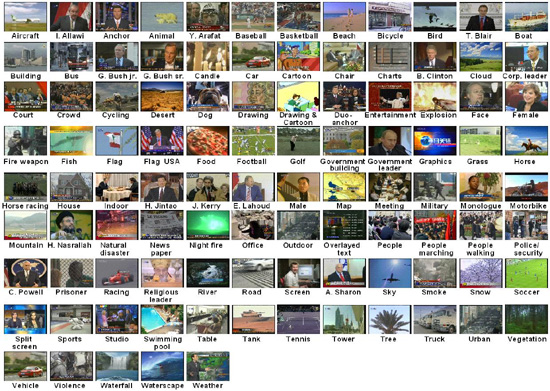
\includegraphics[width=.9\linewidth]{figures/mediamill.jpg}
	\centering
	\caption{Los 101 conceptos semánticos asociados a la colección
		Mediamill.}
	\label{fig:mediamill}
\end{figure}

Estas son solo tres de las colecciones usualmente abordadas en la literatura y
se han seleccionado con el objetivo de diversificar el análisis. Enron es una
colección de pocas instancias pero muchas etiquetas, 20ng a la inversa, cuenta
con pocas etiquetas pero muchas instancias; y Mediamill, finalmente, es la
colección con más instancias que hay disponible y cuenta también con un número
relativamente alto de etiquetas.

Durante la ejecución de experimentos, cada colección será convertida a un flujo
sintético. Además, se generará una versión sintética de cada una, siguiendo la
técnica descripta en la sección \ref{generacion_flujos_sinteticos}.

\section{Software}

A continuación se describen las herramientas de software que fueron utilizadas
para la implementación y ejecución de los experimentos.

\begin{description}

	\item[scikit-multiflow]\footnote{\url{https://scikit-multiflow.github.io/}} Es
	      una librería disponible para el lenguaje de programación Python que provee
	      un \textit{framework} para implementar y comparar algoritmos de aprendizaje
	      automático en ambientes de flujos continuos de datos. Incluye pero no se
	      limita a problemas de clasificación multi-etiquetas
	      \cite{montiel_scikit-multiflow_2018}.

	\item[\acrshort{moa}]\footnote{\url{https://moa.cms.waikato.ac.nz/}}
	      \acrfull{moa} es un \textit{framework} para realizar minería de datos sobre
	      flujos continuos de datos, implementada en Java y de código libre.  Incluye
	      algoritmos de evaluación y de aprendizaje automático como clasificadores,
	      regresores, o de \textit{clustering}, pudiendo ser aplicados a problemas de
	      clasificación de etiqueta única o multi-etiquetas.  También incluye
	      herramientas para generar datos sintéticos. Tanto \acrshort{moa} como
	      scikit-multiflow facilitan la reiteración de experimentos con distintas
	      configuraciones, así como la comparación de resultados y la extensión de
	      funcionalidad \cite{bifet_moa_2010}.

	\item[scikit-learn]\footnote{\url{http://scikit-learn.org/stable/index.html}}
	      Es una librería del lenguaje de programación Python que brinda
	      herramientas para realizar evaluación, visualización y análisis de
	      resultados \cite{pedregosa_scikit-learn_2018}.

	\item[Mulan]\footnote{\url{http://mulan.sourceforge.net/index.html}} Es una
	      librería del lenguaje Java especializada en aprendizaje por
	      multi-etiquetas. Mulan incluye una variedad de colecciones de datos
	      multi-etiquetas que han sido la fuente de otros trabajos de la literatura
	      \cite{tsoumakas_mulan_2011}.

\end{description} \todo{nombres de herramientas van en cursiva?}

La herramienta \acrshort{moa} es usada para generar los flujos sintéticos y
provee del marco de trabajo en el cual se implementó el algoritmo de generación
descripto en \ref{generacion_flujos_sinteticos}. Los algoritmos de clasificación
fueron implementados en Python y están disponibles bajo la librería
\textit{scikit-multiflow}. La solución de ensamble \acrshort{efmp} también fue
implementada en esta librería. \textit{Scikit-learn}, por su parte, provee la
implementación de las métricas basadas en etiquetas, y las colecciones de datos
fueron extraídas de Mulan.

\section{Hardware}

Se ha recibido apoyo del \acrfull{cidetic}, el cual ha proveído de equipos de
altas prestaciones que han proporcionado la capacidad de cómputo necesaria para
llevar a cabo este proyecto. El equipamiento facilitado cuenta con dos nodos de
12 núcleos cada uno, el CPU es un Intel Xeon X5675 de 3.07 GHz de velocidad de
procesamiento, 12 Mb de memoria caché y 6 núcleos. El espacio de almacenamiento
disponible es de 1 Tb y la memoria RAM es de 142 Gb. \todo{Chequear estos datos}

El Sistema Operativo instalado es Ubuntu 18.04 LTS y cuenta con la versión 3.6.9
de Python, el instalador de paquetes Pip en su versión 20.3.3 y Java 1.8.

\section{Algoritmos}
\label{experimentos_algoritmos}

Se realizan los experimentos usando algoritmos multi-etiquetas disponibles en la
librería scikit-multiflow junto con las implementaciones de ensambles
presentadas en este trabajo: \acrfull{efmp} y su variación \acrshort{efmp2}.
Entre los algoritmos del tipo de transformación del problema se seleccionan los
de \acrfull{br}, \acrfull{cc} y \acrfull{mlht}. Tanto \acrshort{br} como
\acrshort{cc} usan \textit{naive} bayes como modelo de clasificación base y
\acrshort{mlht} es ejecutado en su versión basada en \acrfull{lp}, siguiendo los
procedimientos de \citeauthor{read_scalable_2012} \cite{read_scalable_2012}.

En lo que respecta a soluciones de ensamble, los modelos de \acrshort{efmp}
contarán ambos con tres clasificadores base, siendo estos los mencionados en el
párrafo anterior, es decir, \acrshort{cc}, \acrshort{br} y \acrshort{mlht}. La
comparación se hará contra el algoritmo \acrfull{dwm}, tal como ha sido definido
por sus autores \cite{kolter_dynamic_2007} pero adaptado a ambientes de
multi-etiquetas (ver sección \ref{tecnica_algoritmo_ensamble}), y se suman al
análisis los algoritmos de \acrfull{ebr} y \acrfull{ecc}, tal como fueron
definidos por \citeauthor{oza_online_2005} \cite{oza_online_2005} y también han
sido extendidos para soportar problemas de \acrshort{mll}
\cite{read_classifier_2011}. Los tres algoritmos de ensamble extraídos de la
literatura son configurados con diez clasificadores base de \textit{naive}
bayes, para imitar los experimentos conducidos por otros autores de la
literatura \cite{osojnik_multi-label_2017, read_scalable_2012,
	buyukcakir_novel_2018}.

La tabla \ref{tab:algoritmos} es un resumen de los algoritmos seleccionados
junto con los clasificadores base configurados, la referencia bibliográfica y la
clave que será usada en las tablas de resultados.

\begin{table}[htbp]
	\centering
	\begin{adjustbox}{max width=\textwidth}
		\begin{tabular}{lllll}
	\toprule
	Clave                                          & Algoritmo                             & Clasificadores base  & Referencia & \\
	\midrule
	\acrshort{br}                                  & \acrlong{br}                          & \textit{naive} bayes
	                                               & \textcite{tsoumakas_multi-label_2007} &                                     \\
	\acrshort{cc}                                  & \acrlong{cc}                          & \textit{naive} bayes &
	\textcite{read_classifier_2011}                &                                                                             \\
	\acrshort{mlht}                                & \acrlong{mlht}                        & \acrfull{ht}         &
	\textcite{read_scalable_2012}                  &                                                                             \\
	\acrshort{efmp}                                & \acrlong{efmp}                        &
	\acrshort{br}, \acrshort{cc} y \acrshort{mlht} &
	Sección \ref{tecnica_algoritmo_ensamble}       &                                                                             \\
	\acrshort{efmp2}                               & \acrlong{efmp2}                       &
	\acrshort{br}, \acrshort{cc} y \acrshort{mlht} &
	Sección \ref{tecnica_algoritmo_ensamble}       &                                                                             \\
	\acrshort{dwm}                                 & \acrlong{dwm}                         &
	\textit{naive} bayes (10 copias)               &
	\textcite{kolter_dynamic_2007}                 &                                                                             \\
	\acrshort{ebr}                                 & \acrlong{ebr}
	                                               & \textit{naive} bayes (10
	copias)                                        &
	\textcite{read_classifier_2011}                &                                                                             \\
	\acrshort{ecc}                                 & \acrlong{ecc}
	                                               & \textit{naive} bayes (10
	copias)                                        &
	\textcite{read_classifier_2011}                &                                                                             \\
	\bottomrule
\end{tabular}

	\end{adjustbox}
	\caption{Métodos de clasificación multi-etiquetas seleccionados para ambientes
		de flujos continuos de datos.}
	\label{tab:algoritmos}
\end{table}

\section{Métricas de Evaluación}

En la evaluación de algoritmos de clasificación se usan el conjunto de métricas
que han sido utilizadas en otros trabajos de la literatura, tanto en escenarios
de flujos \cite{sousa_multi-label_2018, zheng_survey_2020,
	osojnik_multi-label_2017} como en \textit{batch} \cite{madjarov_extensive_2012,
	zhang_multi-label_2010, gibaja_tutorial_2015} y fueron descriptas en la
sección \ref{mll_evaluacion}. Estas son:

\begin{description}

	\item[Métricas Basadas en Ejemplos]: \textit{Hamming score}, \textit{hamming
		      loss}, \textit{exact-match} (exactitud del subconjunto),
	      \textit{accuracy} (o exactitud, o \textit{jaccard index}), precisión,
	      \textit{recall} (o exhaustividad) y \textit{f1}.

	\item[Métricas Basadas en Etiquetas]: \textit{Accuracy} (micro), precisión
	      (micro), \textit{recall} (micro), \textit{f1} (micro),
	      \textit{accuracy} (macro), precisión (macro), \textit{recall} (macro)
	      y \textit{f1} (macro).

	\item[Métricas de Eficiencia]: Velocidad y tamaño del modelo.

\end{description}

La medición de velocidad comienza en el momento que inicia la predicción y
entrenamiento del modelo por primera vez y finaliza cuando el clasificador
termina de procesar la última instancia de la colección. Por lo tanto, quedan
afuera las etapas de evaluación, carga de la colección en memoria, generación
del flujo y configuración del entrenamiento. El consumo de memoria también es
monitoreado durante la ejecución del entrenamiento y predicción y toma en cuenta
la estructura completa del modelo y todos sus componentes, incluyendo pesos e
hiper-parámetros propios y de sus clasificadores base.

Los flujos sintéticos son analizados teniendo en cuenta los fenómenos propios de
colecciones del mundo real. A ese fin se estudia el sesgo de etiquetas, la
relación entre etiquetas, la distribución de etiquetas y el espacio de atributos
(ver sección \ref{mll_fenomenos}). \todo{es probable que este análisis se separe
	en una sección aparte y se aborde con mayor profundidad}

\section{Configuración Experimental}

En lo que respecta a modelos de aprendizaje automático, los experimentos fueron
desarrollados en el lenguaje Python usando la librería
\textit{scikit-multiflow}. Los algoritmos de transformación del problema se
aplican tal como han sido implementados en la librería con la salvedad del
\acrshort{mlht}, al que debió introducirle una modificación para manipular la
predicción, se usaba un arreglo disperso para representar las etiquetas
activadas, lo cual producía un desbordamiento de memoria en el entrenamiento de
colecciones grandes como la de Mediamill. Se lo suplantó por una estructura de
representación densa. En cuanto a los modelos de ensambles, se adaptaron las
implementaciones existentes de \acrshort{ebr}, \acrshort{ecc} y \acrshort{dwm}
para soportar múltiples etiquetas y para ello se debió modificar la etapa de
combinación de votos para hacer frente a la nueva dimensionalidad de los datos.
Por lo demás, la configuración de los algoritmos es la definida en la sección
\ref{experimentos_algoritmos}.

Para la etapa de evaluación se aplica la técnica de evaluación secuencial
predictiva (\textit{prequential}) con ventanas deslizantes, tal como se
recomienda para ambientes de flujos continuos \cite{gama_evaluating_2013}. Ante
cada ejemplo o ventana de ejemplos arribada el modelo primero realiza la
predicción y luego el entrenamiento. Finalmente las métricas de evaluación son
calculadas una vez procesados todos los ejemplos de la colección y a partir de
todas las predicciones producidas.  Notar que a partir de esta técnica el modelo
predice y entrena todas las instancias, y no solo un subconjunto de ellas como
sucede con la estrategia de \textit{holdout}. La ventana deslizante se configura
en $w = \frac{N}{20}$, es decir, se divide el número total de instancias del
flujo en 20 ventanas, siguiendo las directivas de \textcite{read_scalable_2012}.
Los resultados de la evaluación son agrupados según los tipos de métrica usados,
para facilitar el análisis.

Por otro lado, los flujo de datos sintéticos fueron generados a partir de las
colecciones 20ng, Enron y Mediamill. Por cada uno de ellos se generan tres
\textit{streams} sintéticos:

\begin{description}

	\item[MOA]: Es un stream generado usando el método de los autores de
	      referencia \cite{read_generating_2009}. El número de instancias es el
	      mismo de la colección original y el generador de atributos es
	      \acrfull{rbf} (ver sección~\ref{stream_syn}).

	\item[JC]: Es un stream generado usando el método presentado en la sección
	      ~\ref{generacion_flujos_sinteticos}. El número de instancias es el
	      mismo de la colección original y el generador de atributos es
	      \acrfull{rbf}.

	\item[JC\_BIG]: Es un stream similar a JC pero cuenta con un mayor número de
	      instancias. La idea es poder determinar si a mayor el tamaño del
	      \textit{stream} mayor es la similitud con la colección original.

\end{description}

Una vez generados estos flujos sintéticos se realizó un análisis para determinar
en qué grado se observan los fenómenos de la colección original en las
colecciones sintéticas. Estos fenómenos son el sesgo de etiquetas, la
distribución de etiquetas y la relación entre etiquetas. \todo{agregar espacio
	de atributos?} y se capturaron de la siguiente manera:

\todo{a completar}
\begin{description}

	\item[Sesgo de etiquetas]: Para observar el sesgo de etiquetas se toma la frecuencia de
	      cada etiqueta y se traza un gráfico de lineas para cada \textit{stream}, de esta
	      manera es posible visualizar cuánto se asemeja el sesgo de los datos sintéticos
	      al de los datos reales.

	\item[Distribución de etiquetas]: a completar.

	\item[Relación entre Etiquetas]: a completar.

\end{description}


\section{Resultados}

\subsection{Flujos Continuos Sintéticos}

\subsubsection{20ng}

\begin{table}[htbp]
	\centering
	\begin{adjustbox}{max width=\textwidth}
		\begin{tabular}{lrrrr}
	\toprule
	\multicolumn{5}{c}{20ng}             \\
	Nombre  & N     & L  & LC    & LD    \\
	\midrule
	20ng    & 19300 & 20 & 1,029 & 0,051 \\
	MOA     & 19300 & 20 & 3,397 & 0,170 \\
	JC      & 19300 & 20 & 1,067 & 0,053 \\
	JC\_BIG & 80000 & 20 & 1,062 & 0,053 \\
	\bottomrule
\end{tabular}

	\end{adjustbox}
	\caption{Características de los \textit{streams} sintéticos generados sobre
		la colección 20ng.  N: número de instancias; L: número de etiquetas; LC:
		cardinalidad de etiquetas; LD: densidad de etiquetas.}
	\label{tab:syn_20ng_stats}
\end{table}

La tabla~\ref{tab:syn_20ng_stats} muestra las características de la colección
original y de los \textit{streams}. Allí se observa que la cardinalidad de la
colección apenas sobrepasa la unidad, lo que significa que la mayoría de sus
instancias tienen una única etiqueta. Esta característica logra ser capturada de
manera aproximada por los \textit{streams} JC y JC\_BIG pero no así por MOA que
asocia más de tres etiquetas por instancia. La
figura~\ref{fig:syn_20ng_label_skew} es una representación gráfica del sesgo de
etiquetas, y muestra que la colección original tiene alrededor de veinte
combinaciones con una frecuencia escalada cercana a la máxima y luego un
descenso brusco que culmina en la combinación 25, desde la cual se mantiene
cercana a la frecuencia escalada mínima. Esta tendencia es bien replicada en los
\textit{streams} JC pero no en MOA, donde el descenso es más escalonado y no
alcanza la zona baja del eje y. La
tabla~\ref{tab:syn_20ng_top_labels_combinations} muestra las principales 5
combinaciones de etiquetas para cada \textit{stream}. Cabe destacar que todas
las combinaciones en la tabla para los \textit{streams} JC y JC\_BIG son de una
etiqueta cada una, tal como el original, pero además JC captura 3 de las 5
combinaciones principales del original: $\{religion.cristian\}$,
$\{rec.sport.hockey\}$ y $\{sci.crypt\}$.

\begin{figure}[htbp]
	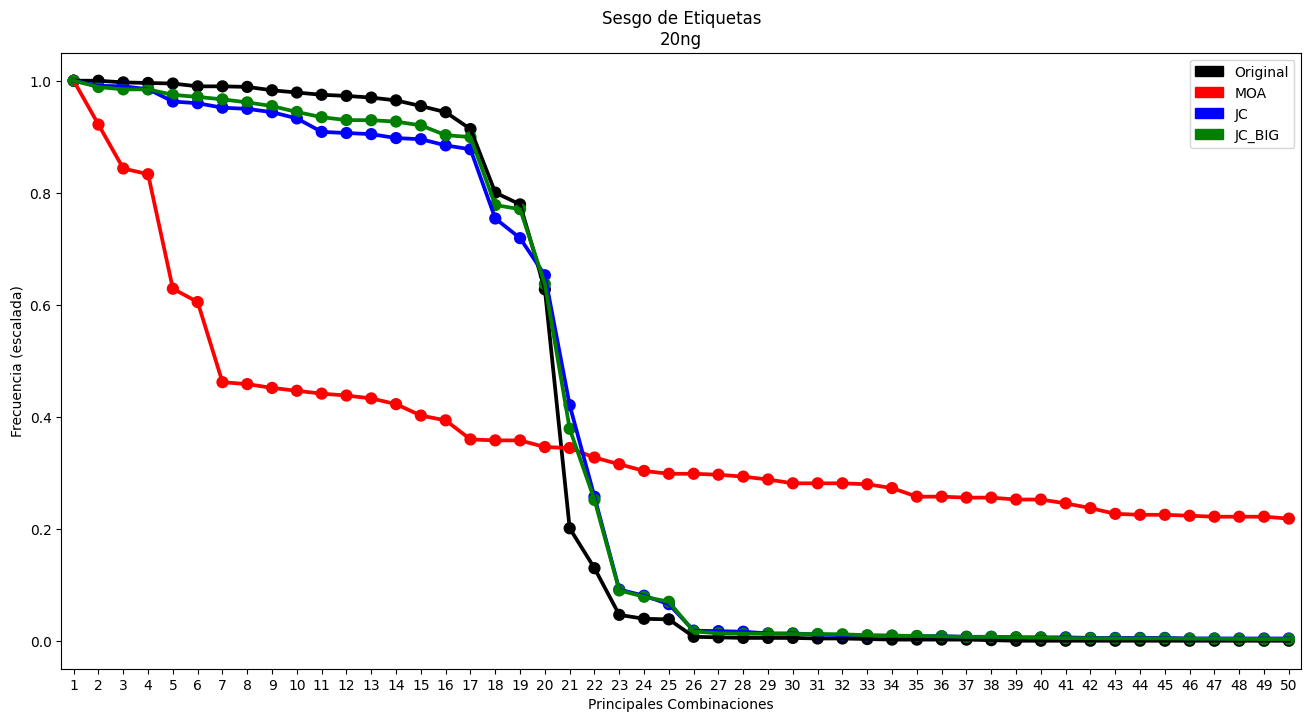
\includegraphics[width=\linewidth]{figures/experiments/syn/20ng/label_skew.png}
	\caption{Sesgo de etiquetas de los \textit{streams} generados sobre la colección
		20ng.}
	\label{fig:syn_20ng_label_skew}
\end{figure}

\begin{table}[htbp]
	\centering
	\begin{adjustbox}{max width=\textwidth}
		\begin{tabular}{lllll}
	\toprule
	\textit{Rank} & Original               & JC                     & JC\_BIG                & MOA                                                                                       \\
	\midrule
	1             & \{religion.christian\} & \{sci.crypt\}          & \{religion.christian\} & \{comp.os\_ms\_windows\_misc, religion.rmisc, misc\_forsale, comp.sys.ibm\_pc\_hardware\} \\[3pt]
	2             & \{rec.sport.hockey\}   & \{sci.med\}            & \{rec.motorcycles\}    & \{sci.space, rec.autos, rec.motorcycles, politics.guns, religion.atheism\}                \\[3pt]
	3             & \{sci.crypt\}          & \{religion.christian\} & \{rec.autos\}          & \{religion.rmisc, sci.space, misc\_forsale\}                                              \\[3pt]
	4             & \{rec.motorcycles\}    & \{sci.electronics\}    & \{sci.med\}            & \{sci.space, rec.motorcycles, politics.guns, religion.atheism\}                           \\[3pt]
	5             & \{rec.sport.baseball\} & \{rec.sport.hockey\}   & \{sci.electronics\}    & \{politics.pmisc, politics.mideast, rec.sport.hockey, sci.crypt\}                         \\
	\bottomrule
\end{tabular}


	\end{adjustbox}
	\caption{Sesgo de etiquetas - Principales combinaciones de los
		\textit{streams} generados sobre la colección 20ng.}
	\label{tab:syn_20ng_top_labels_combinations}
\end{table}

La figura~\ref{fig:syn_20ng_label_distribution} representa de manera gráfica la
distribución de las etiquetas. Allí se observa cómo los \textit{streams} aquí
presentados reproducen con eficacia la composición de la cardinalidad a lo largo
de los distintos tamaños de conjuntos de etiquetas. El gráfico de \textit{mean
	absolute error} ayuda a reforzar esta idea. En cuanto al tipo de distribución,
del cual se hace mención en el trabajo de referencia, los \textit{streams} JC y
JC\_BIG, tanto como el original, obedecen al tipo A, esto es, la mayoría de los
ejemplos tienen un conjunto de etiquetas de cardinalidad uno.


\begin{figure}[htbp]
	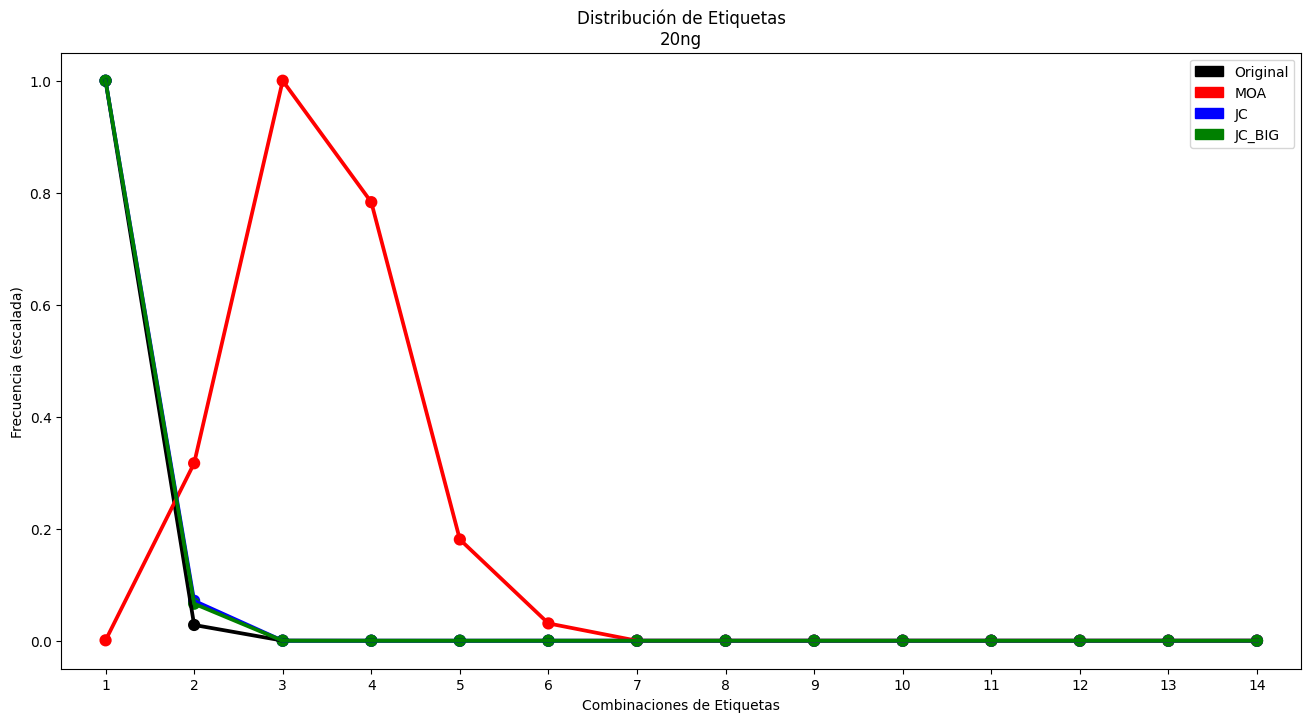
\includegraphics[width=\linewidth]{figures/experiments/syn/20ng/label_distribution.png}
	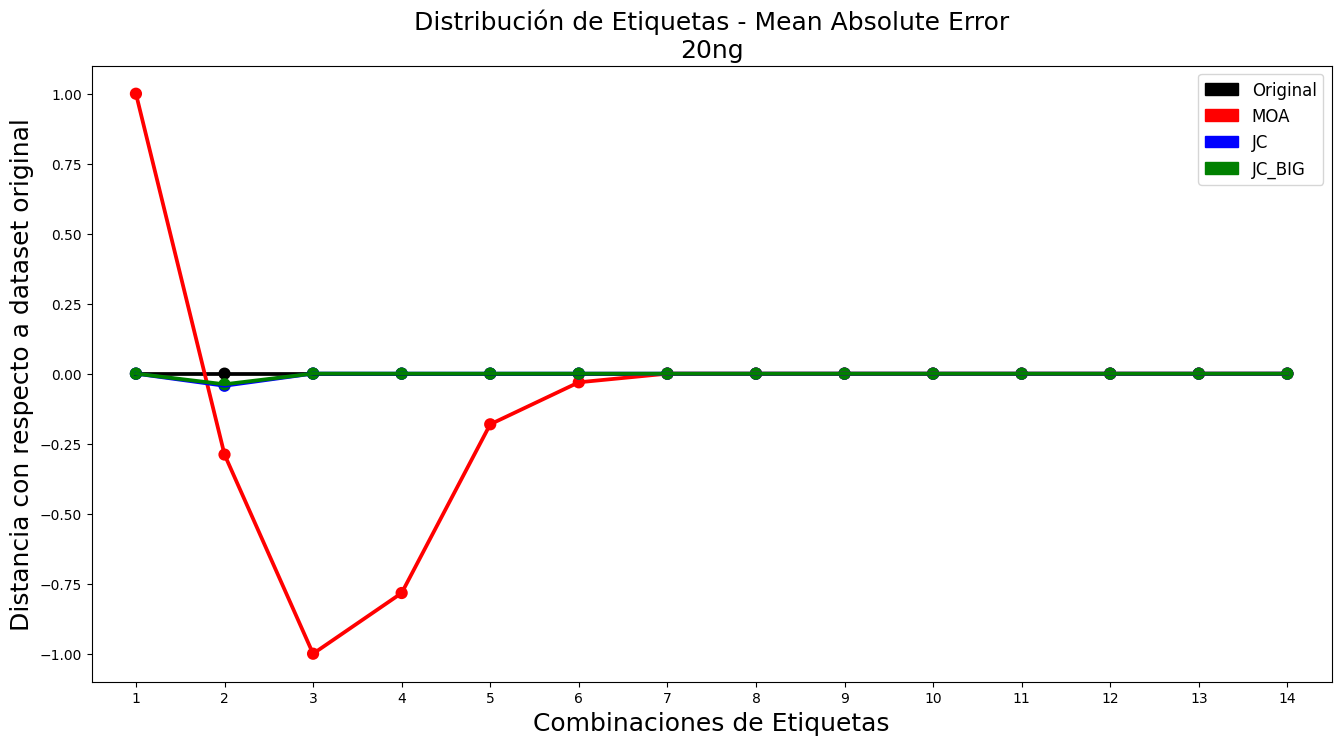
\includegraphics[width=\linewidth]{figures/experiments/syn/20ng/ld_mae.png}
	\caption{Distribución de etiquetas de los \textit{streams} generados sobre la colección
		20ng. Arriba se encuentra el gráfico con las frecuencias escaladas y
		abajo el \textit{mean absolute error} entre cada \textit{stream} y la
		colección original.}
	\label{fig:syn_20ng_label_distribution}
\end{figure}

Finalmente, la figura~\ref{fig:syn_20ng_label_relationship} es una
representación visual de la dependencia entre etiquetas. Ambos ejes del gráfico
constan de las etiquetas de la colección y cuánto mayor es la tonalidad de
blanco en la celda, mayor es la dependencia entre las dos etiquetas. Para 20ng
los gráficos de la colección original, JC y JC\_BIG, son casi idénticos entre sí
por lo que es posible aseverar que el uso de la matriz de correlaciones en la
generación de \textit{streams} sintéticos ha contribuido a reproducir el
fenómeno de la dependencia entre etiquetas para esta colección.

\begin{figure}[htbp]
	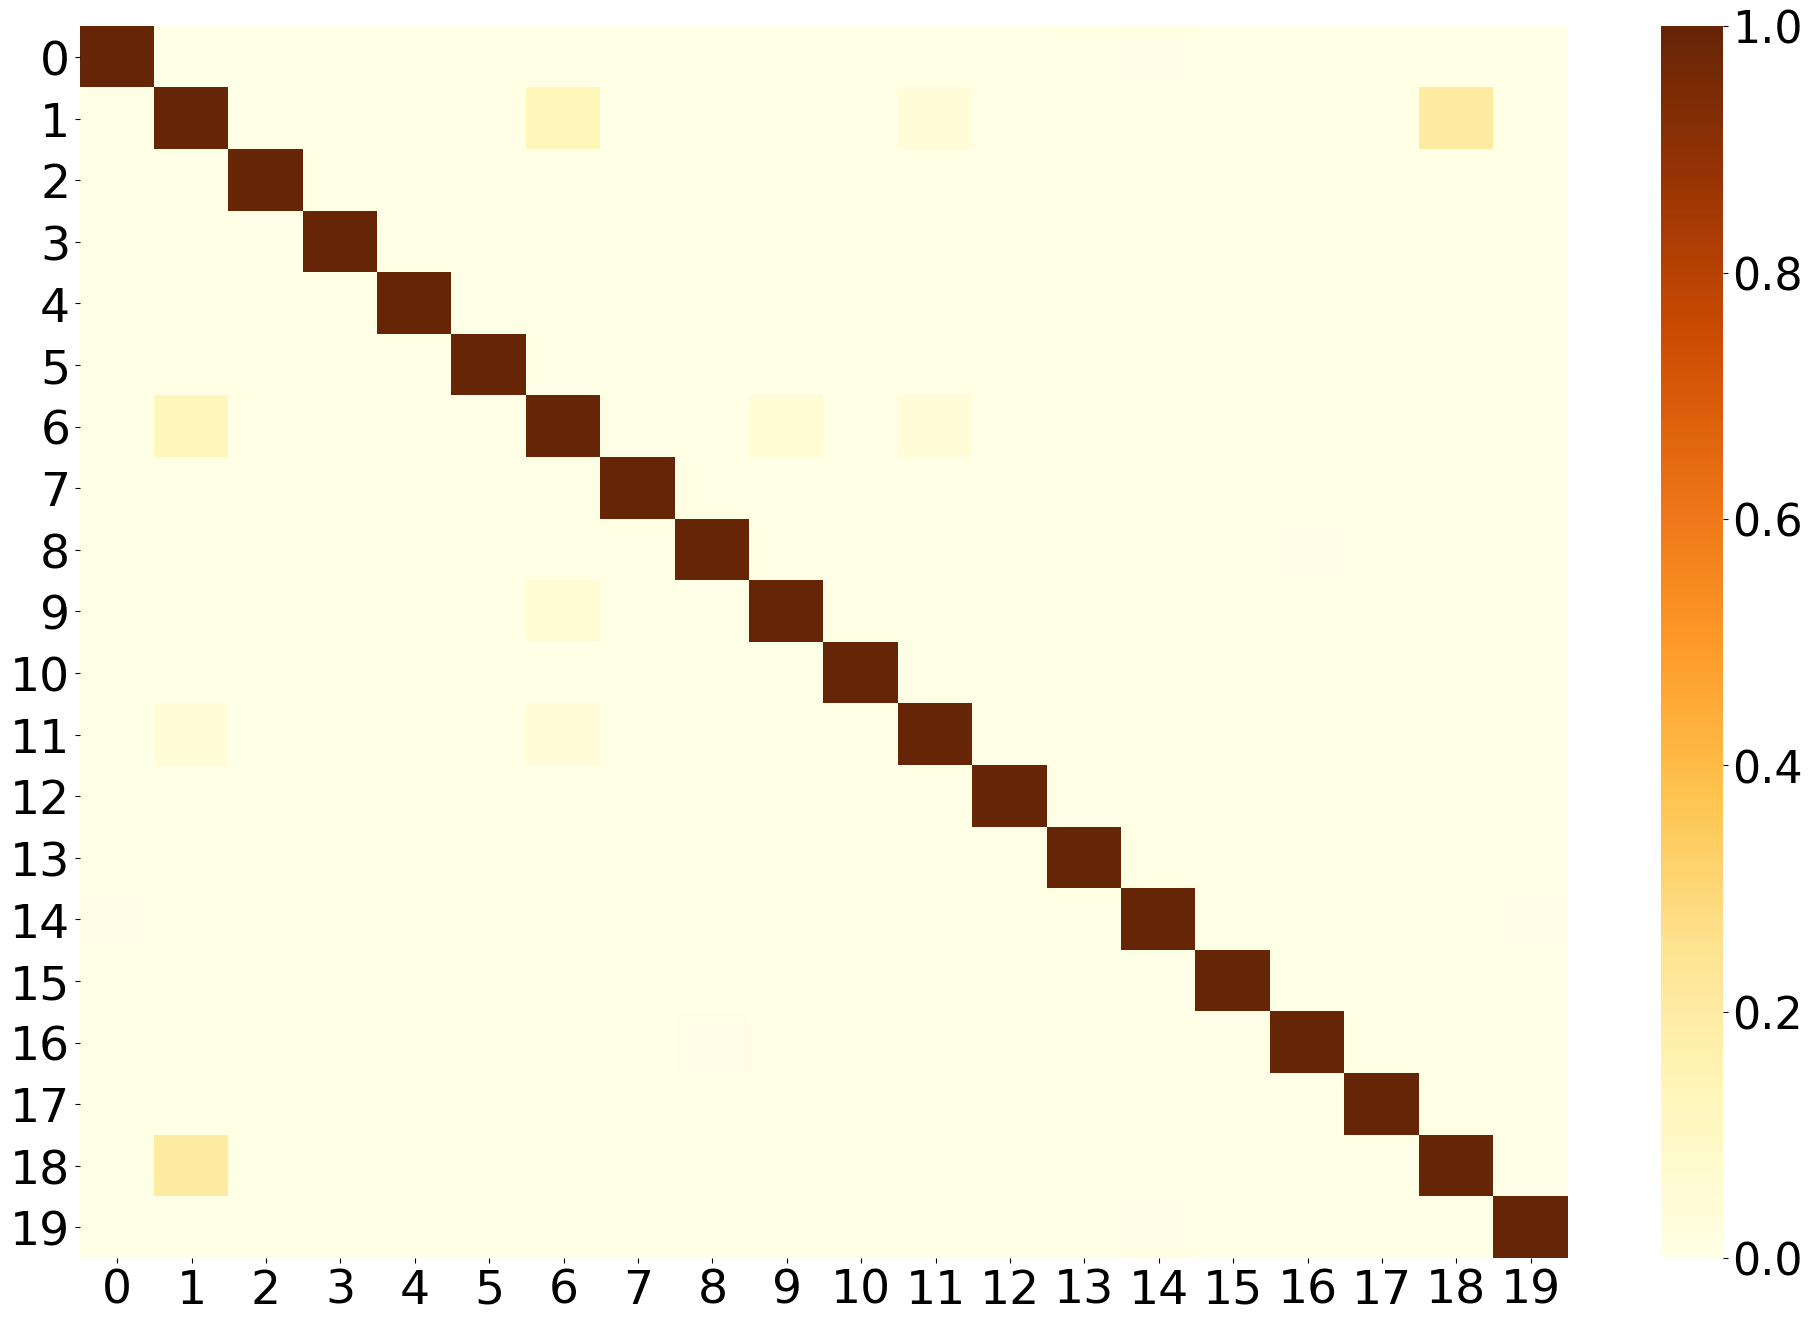
\includegraphics[width=\linewidth / 2]{figures/experiments/syn/20ng/20ng_relationship_graph.png}
	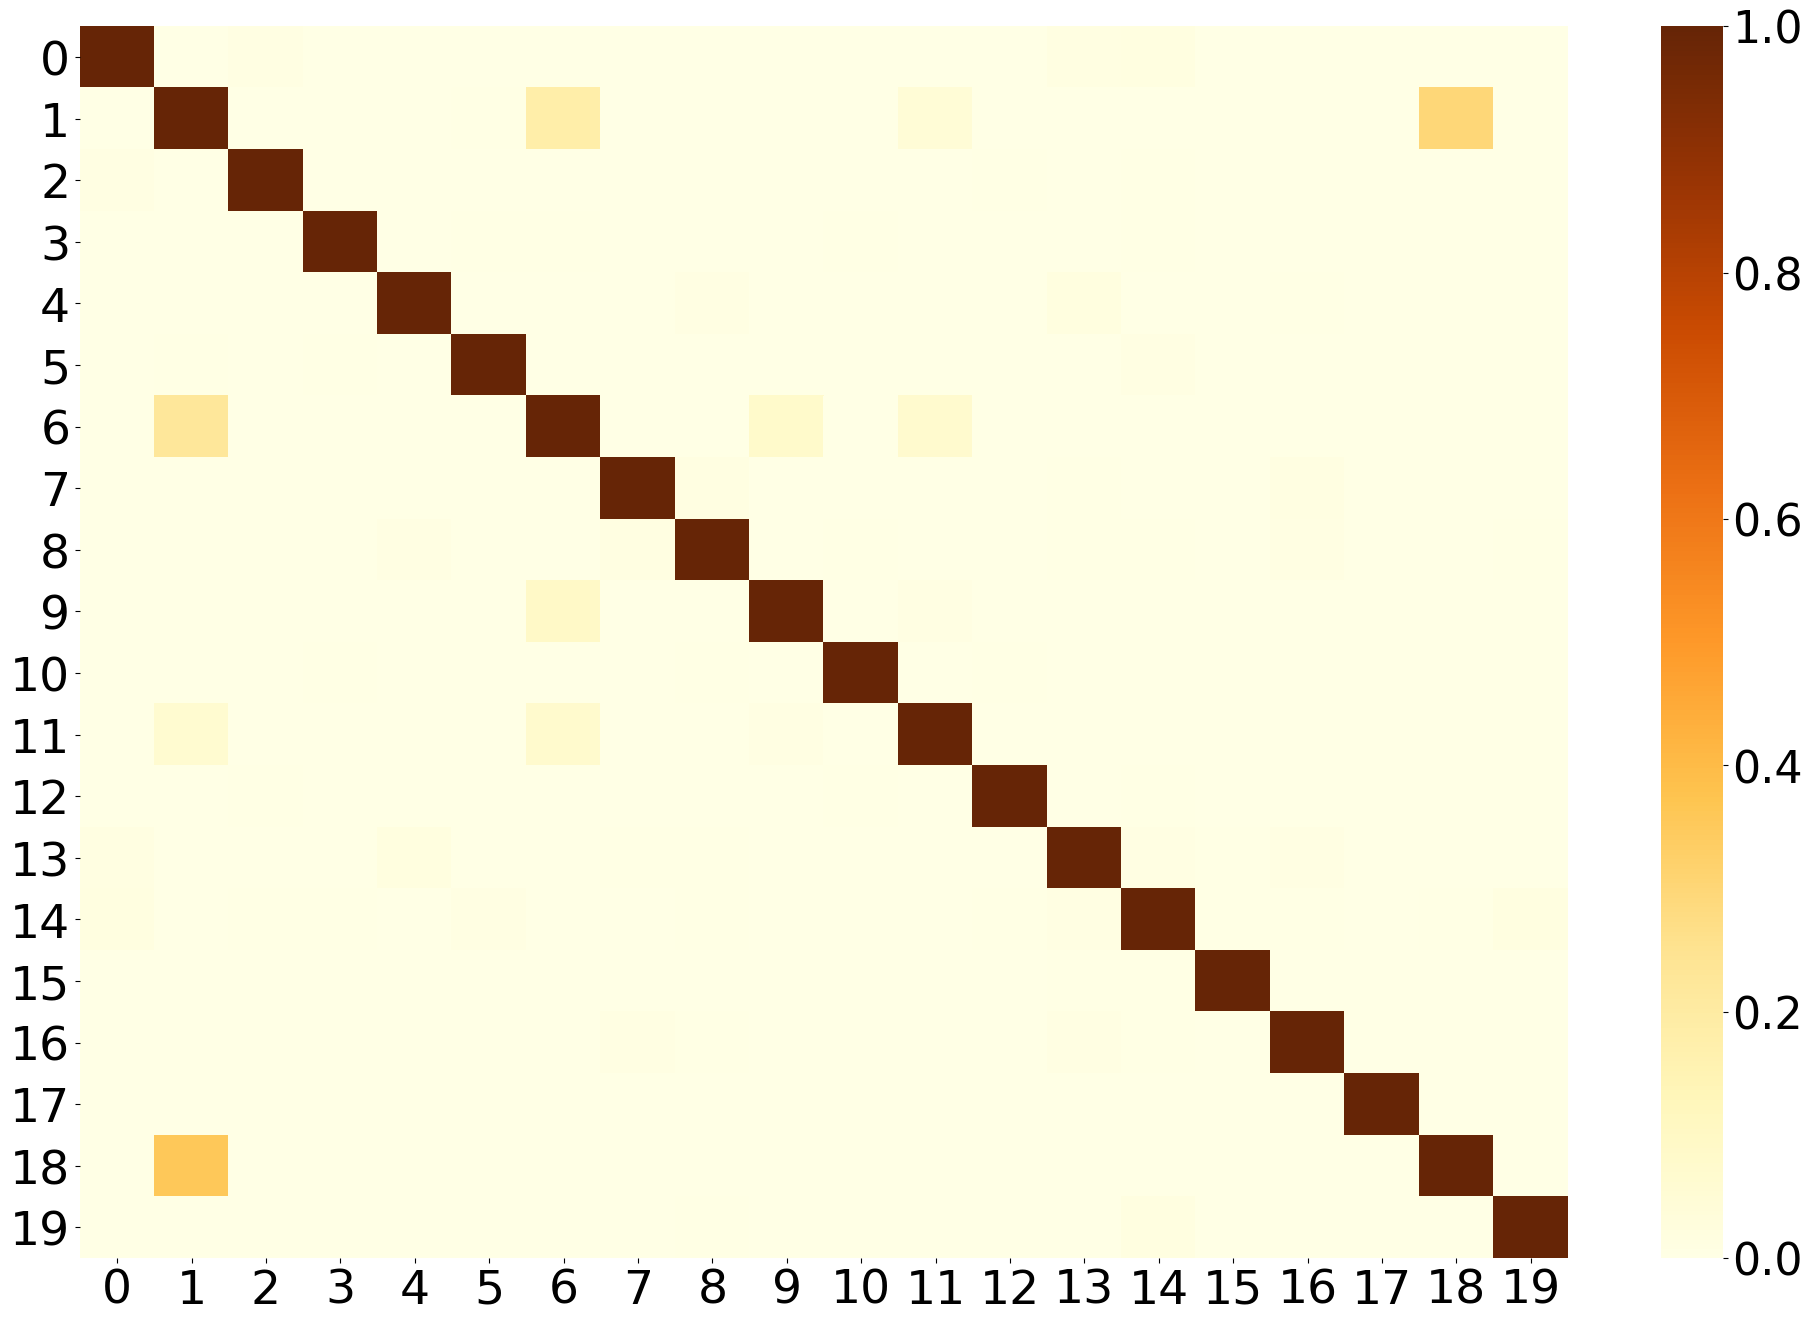
\includegraphics[width=\linewidth / 2]{figures/experiments/syn/20ng/JC_relationship_graph.png}
	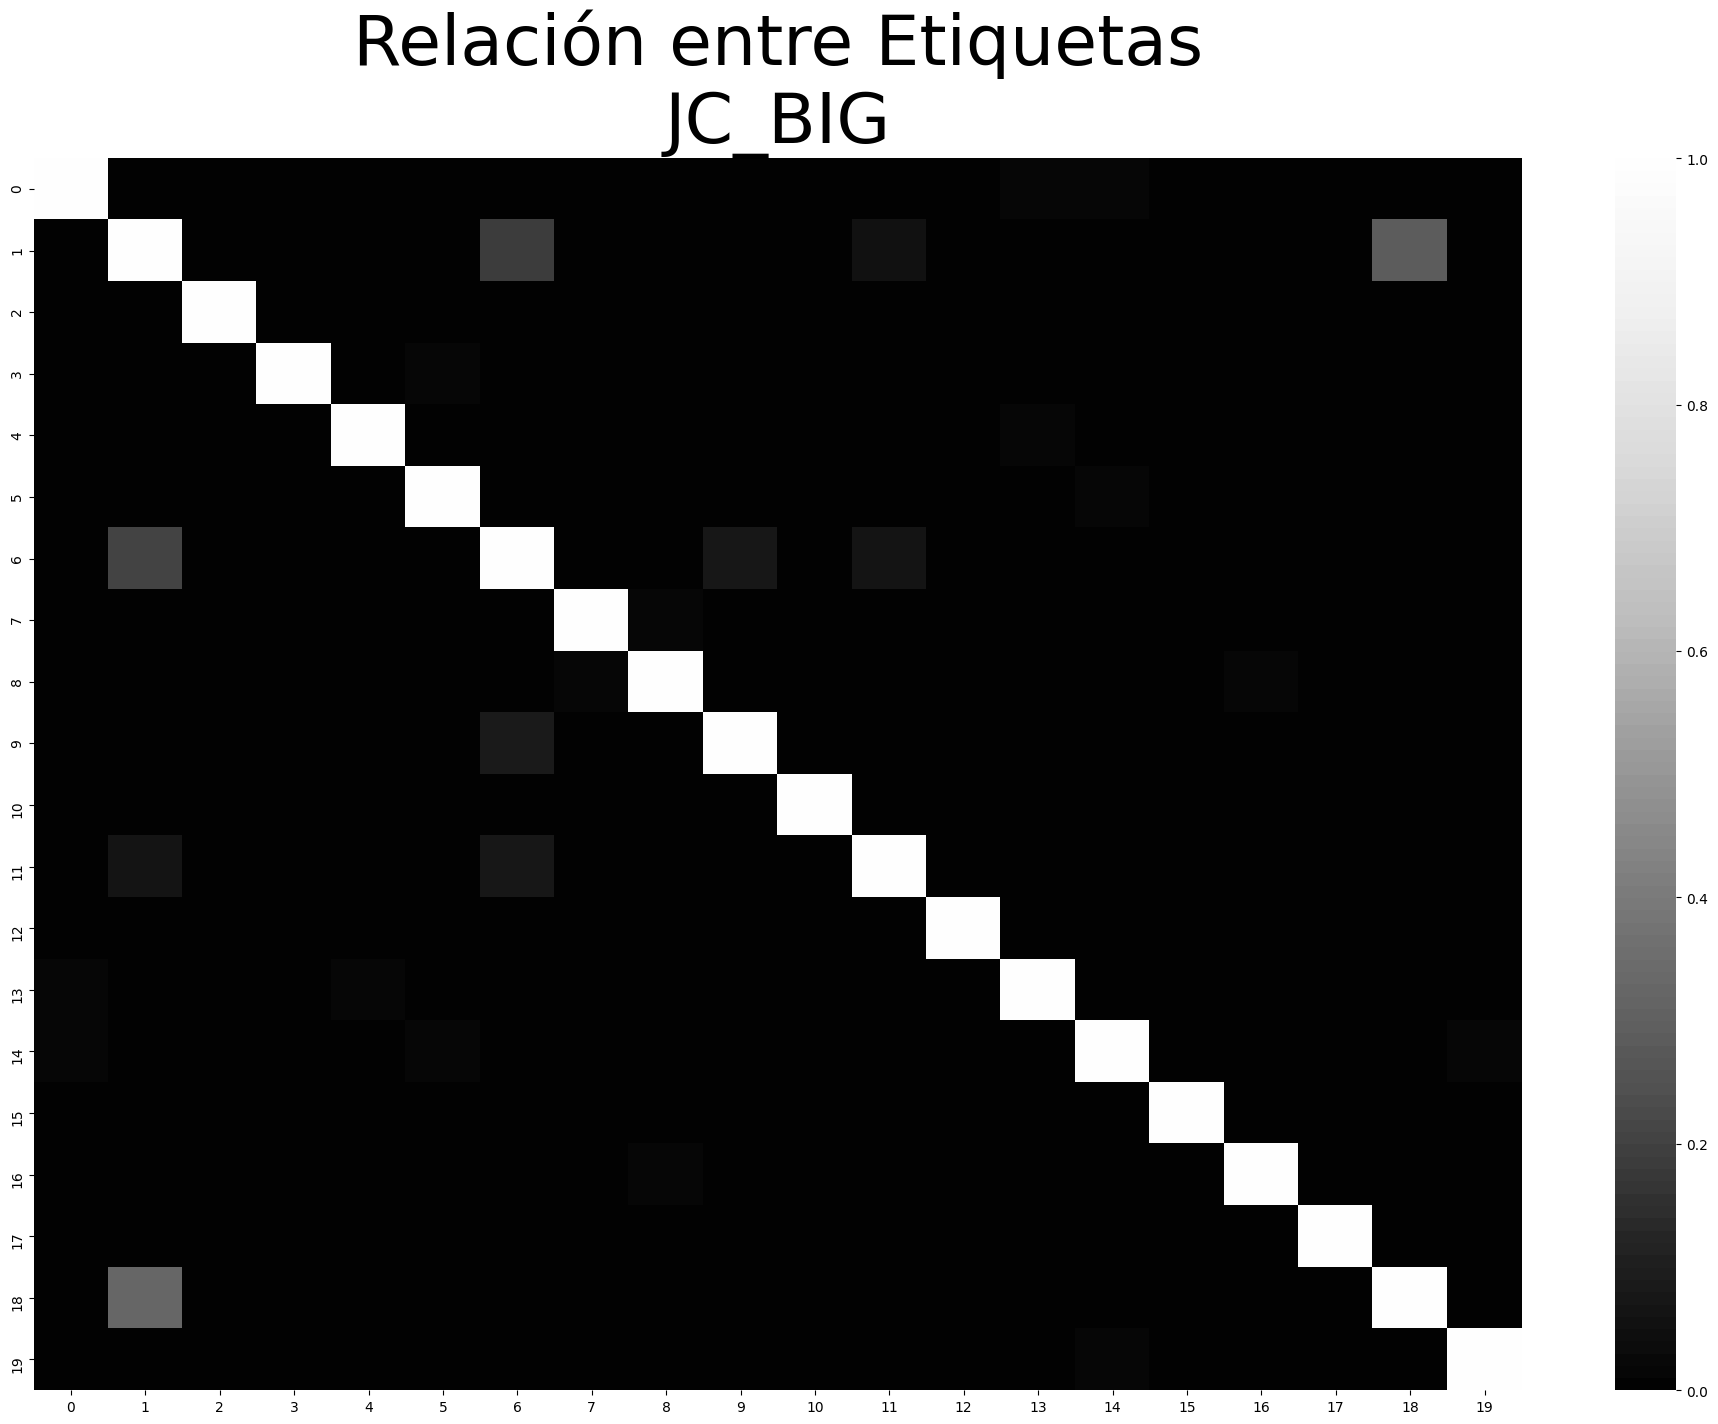
\includegraphics[width=\linewidth / 2]{figures/experiments/syn/20ng/JC_BIG_relationship_graph.png}
	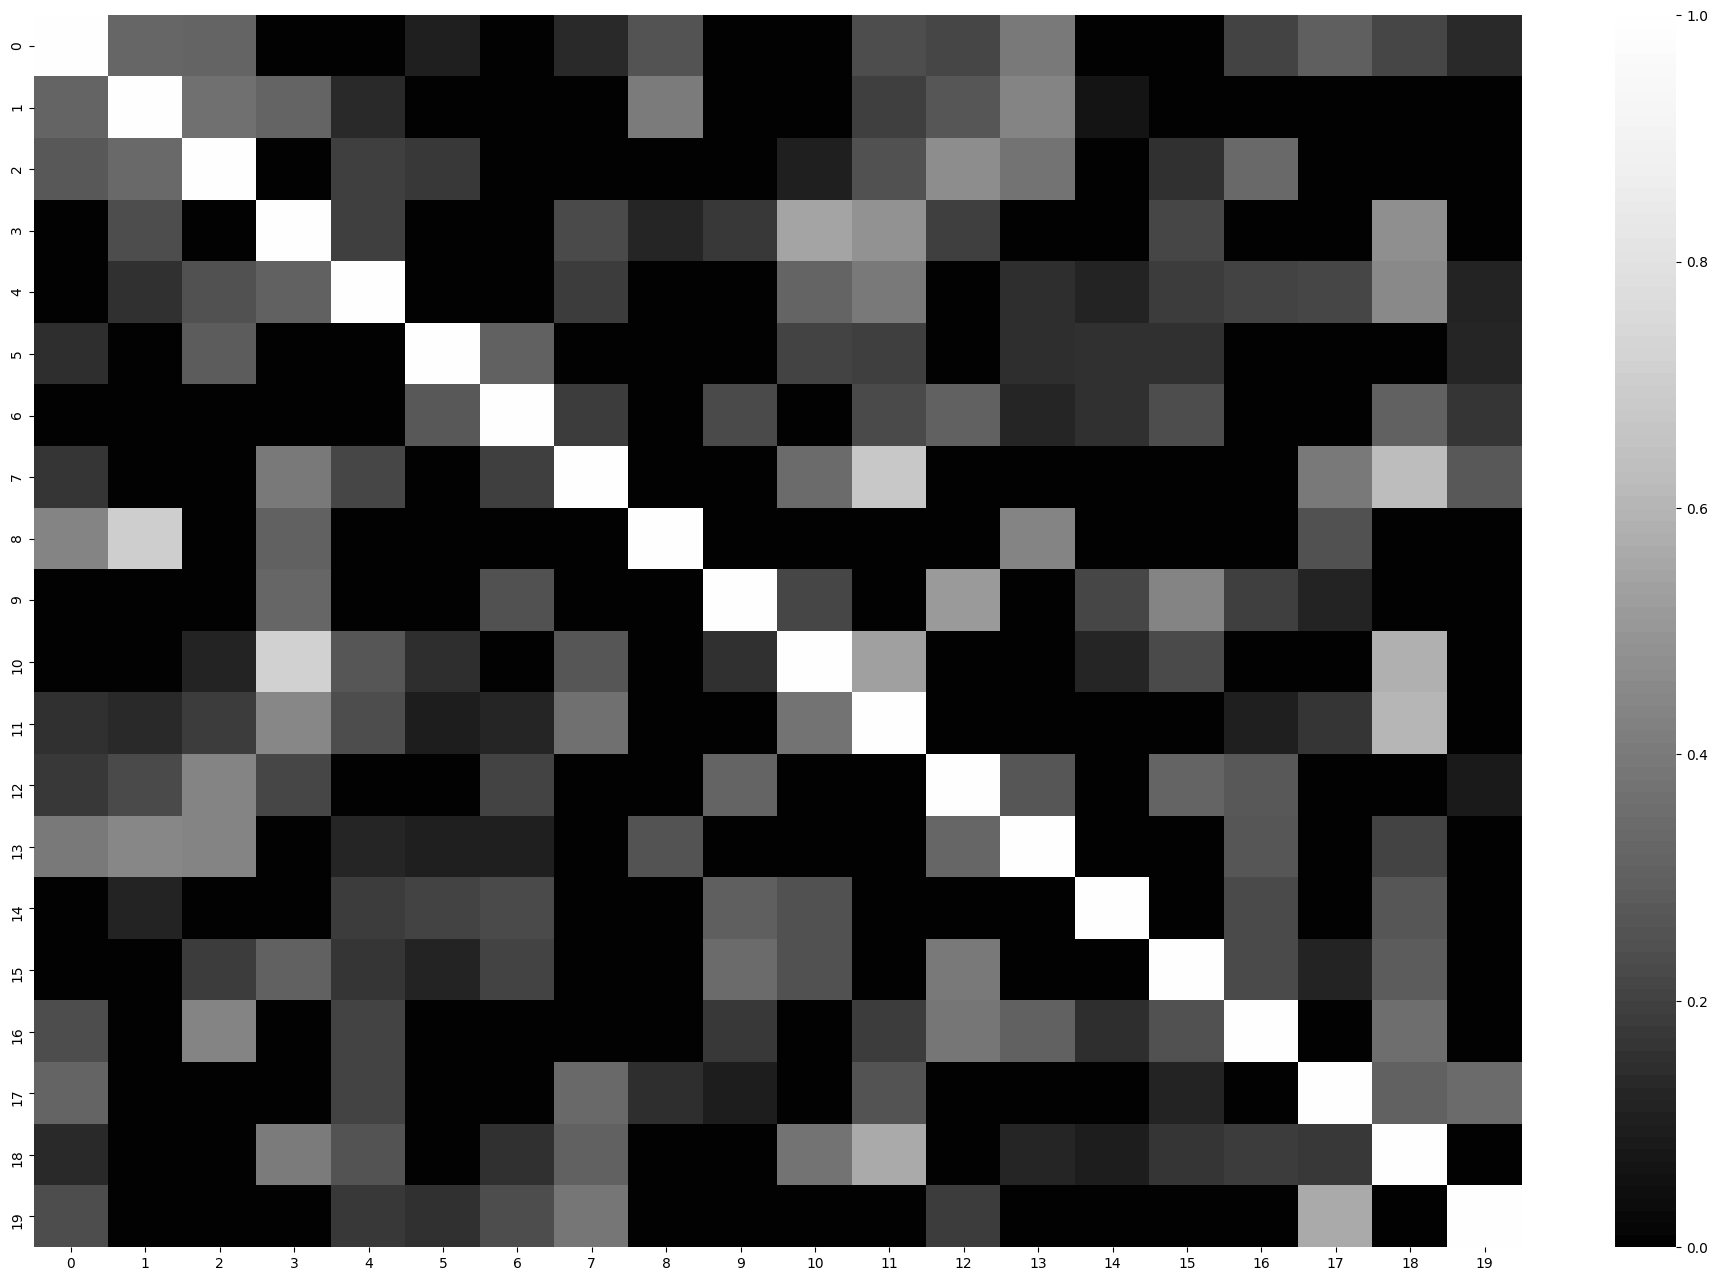
\includegraphics[width=\linewidth / 2]{figures/experiments/syn/20ng/MOA_relationship_graph.png}
	\caption{Relación entre etiquetas para cada \textit{stream} generado sobre
		la colección 20ng. Arriba a la izquierda: \textit{Stream} original. Arriba a la
		derecha: \textit{Stream} JC. Abajo a la izquierda: \textit{Stream}
		JC\_BIG. Abajo a la derecha: \textit{Stream} MOA.}
	\label{fig:syn_20ng_label_relationship}
\end{figure}

\subsubsection{Enron}

\begin{table}[htbp]
	\centering
	\begin{adjustbox}{max width=\textwidth}
		\begin{tabular}{lrrrr}
	\toprule
	\multicolumn{5}{c}{Enron}             \\
	Nombre  & N      & L  & LC    & LD    \\
	\midrule
	Enron   & 1702   & 53 & 3,378 & 0,064 \\
	MOA     & 1702   & 53 & 3,707 & 0,070 \\
	JC      & 1702   & 53 & 2,330 & 0,044 \\
	JC\_BIG & 100000 & 53 & 2,321 & 0,044 \\
	\bottomrule
\end{tabular}

	\end{adjustbox}
	\caption{Características de los \textit{streams} sintéticos generados sobre
		la colección Enron.  N: número de instancias; L: número de etiquetas; LC:
		cardinalidad de etiquetas; LD: densidad de etiquetas.}
	\label{tab:syn_enron_stats}
\end{table}

Partiendo de la tabla~\ref{tab:syn_enron_stats} se observa que el
\textit{stream} MOA se aproxima más al valor de cardinalidad de la colección
original que nuestra propuesta. Sin embargo, JC Y JC\_BIG, describen una curva
en el gráfico de la figura~\ref{fig:syn_enron_label_skew} que, en comparación
con MOA, tiene una mayor similitud con la curva de la colección original.  Se
adjunta la tabla~\ref{tab:syn_enron_top_labels_combinations} como complemento al
estudio del sesgo.

\begin{figure}[htbp]
	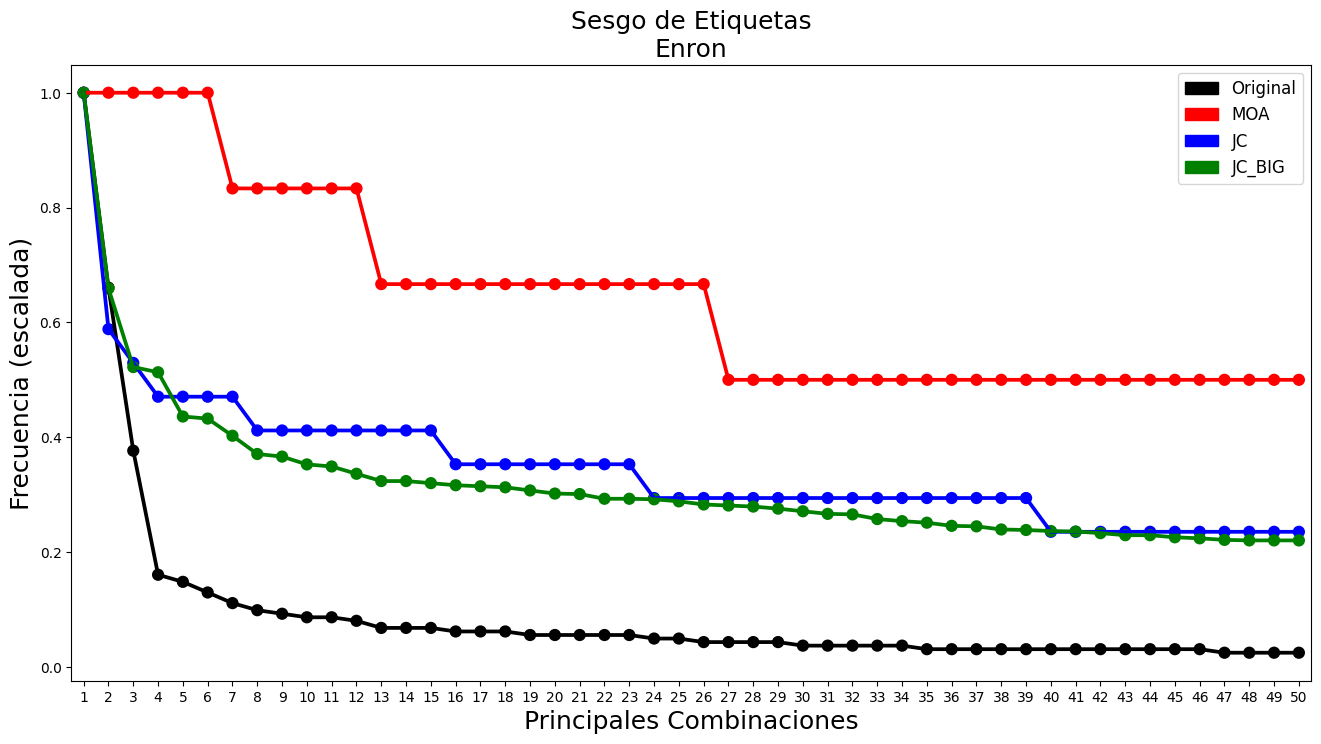
\includegraphics[width=\linewidth]{figures/experiments/syn/enron/label_skew.png}
	\caption{Sesgo de etiquetas de los \textit{streams} generados sobre la colección
		Enron.}
	\label{fig:syn_enron_label_skew}
\end{figure}

\begin{table}[htbp]
	\centering
	\begin{adjustbox}{max width=\textwidth}
		\begin{tabular}{lllll}
	\toprule
	\textit{Rank} & Original             & JC               & JC\_BIG          & MOA                           \\
	\midrule
	1             & \{A.A4\}             & \{A.A4, C.C13\}  & \{A.A4, C.C13\}  & \{B.B12, B.B4, D.D10, C.C1\}  \\
	2             & \{B.B2, A.A4, B.B1\} & \{C.C10, D.D18\} & \{A.A6, D.D18\}  & \{D.D1, A.A5, D.D5, B.B10\}   \\
	3             & \{B.B2, A.A4\}       & \{A.A4, D.D4\}   & \{C.C10, D.D18\} & \{A.A8, B.B3, D.D16, B.B9\}   \\
	4             & \{A.A1, B.B4, C.C6\} & \{A.A7, B.B13\}  & \{A.A7, B.B13\}  & \{C.C7, D.D13, D.D10, D.D18\} \\
	5             & \{B.B2, A.A5, B.B1\} & \{A.A4, B.B9\}   & \{A.A1, D.D18\}  & \{C.C5, B.B2, A.A6, D.D15\}   \\
	\bottomrule
\end{tabular}


	\end{adjustbox}
	\caption{Sesgo de etiquetas - Principales combinaciones de los
		\textit{streams} generados sobre la colección Enron.}
	\label{tab:syn_enron_top_labels_combinations}
\end{table}

Con respecto a la distribución de etiquetas
(figura~\ref{fig:syn_enron_label_distribution}) no es posible determinar si
alguno de los \textit{streams} refleja el fenómeno en mayor grado que otro. Al
mismo tiempo, si bien ninguno de ellos logra reproducir con exactitud la
composición de la cardinalidad entre conjuntos de etiquetas, hay un grado de
similitud entre curvas (ver gráfico de \textit{mean absolute error}) que podría
ser aceptable, dependiendo de la tarea a resolver. En cuanto al tipo de
distribución, del cual se hace mención en el trabajo de referencia, todos los
\textit{streams} sintéticos obedecen al tipo B, es decir, la mayoría de los
ejemplos tienen una cardinalidad de etiquetas mayor que uno.

\begin{figure}[htbp]
	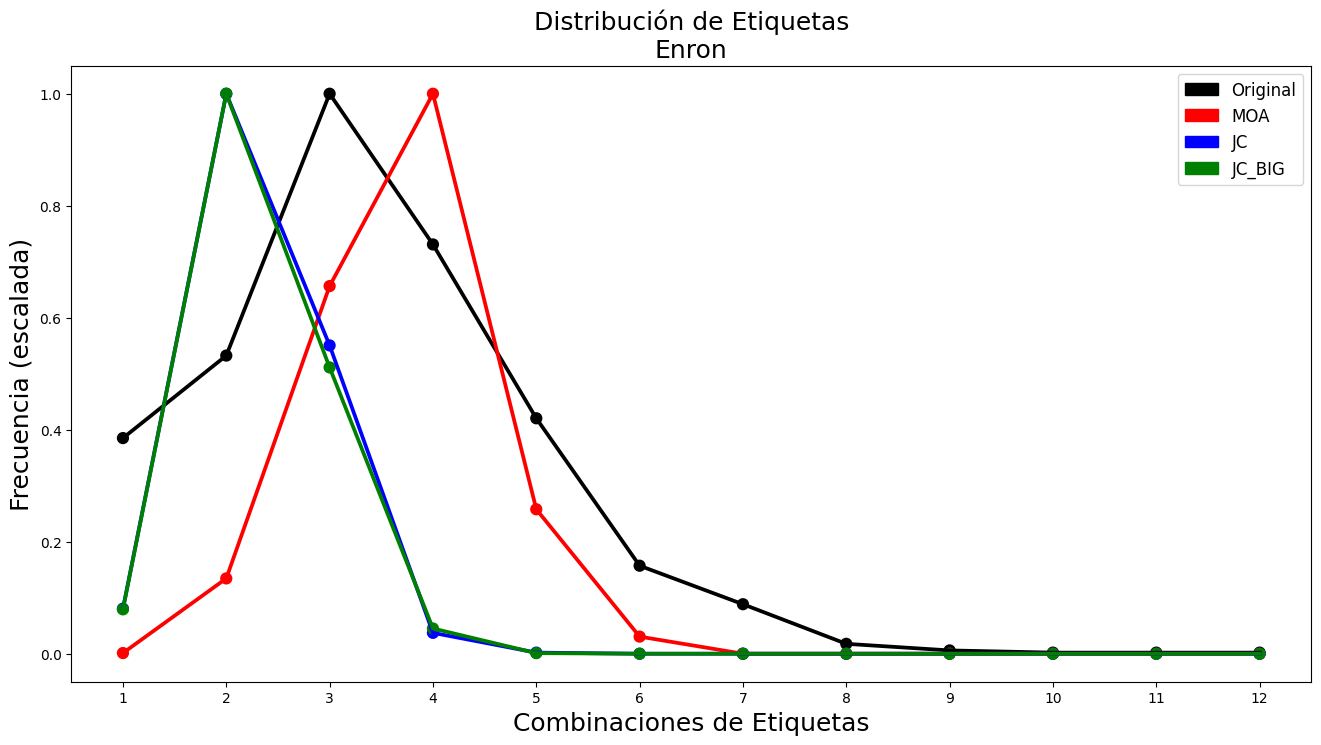
\includegraphics[width=\linewidth]{figures/experiments/syn/enron/label_distribution.png}
	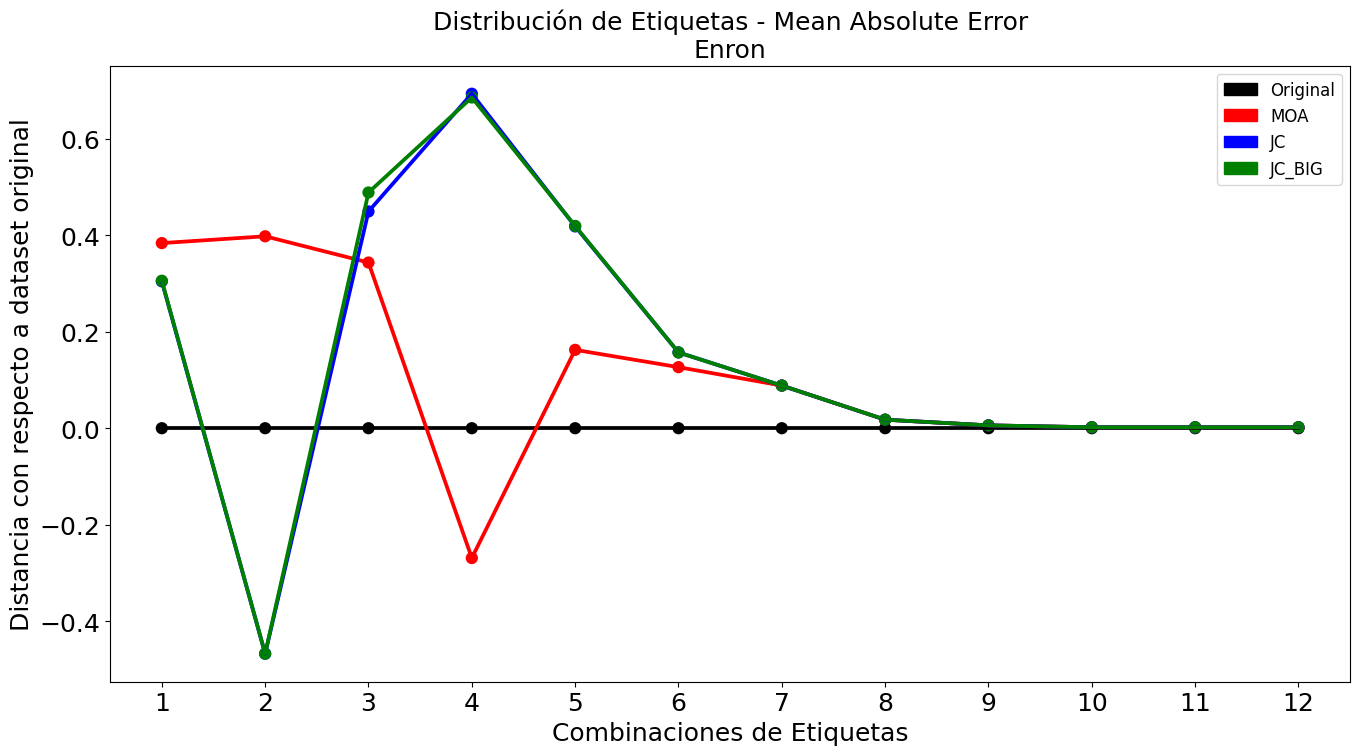
\includegraphics[width=\linewidth]{figures/experiments/syn/enron/ld_mae.png}
	\caption{Distribución de etiquetas de los \textit{streams} generados sobre la colección
		Enron. Arriba se encuentra el gráfico con las frecuencias escaladas y
		abajo el \textit{mean absolute error} entre cada \textit{stream} y la
		colección original.}
	\label{fig:syn_enron_label_distribution}
\end{figure}

Por último, el fenómeno de la dependencia entre etiquetas es representado
visualmente por la figura~\ref{fig:syn_enron_label_relationship}. Tal como
sucedió con la colección 20ng, los gráficos de JC y JC\_BIG para Enron reflejan
una coloración muy similar al del original, aunque con una tonalidad de blanco
menos intensa. Este comportamiento podría estar emparentado con la cardinalidad
de etiquetas, que en estos \textit{streams} sintéticos es menor. No obstante, se
requieren más estudios para arribar a una conclusión al respecto.

\begin{figure}[htbp]
	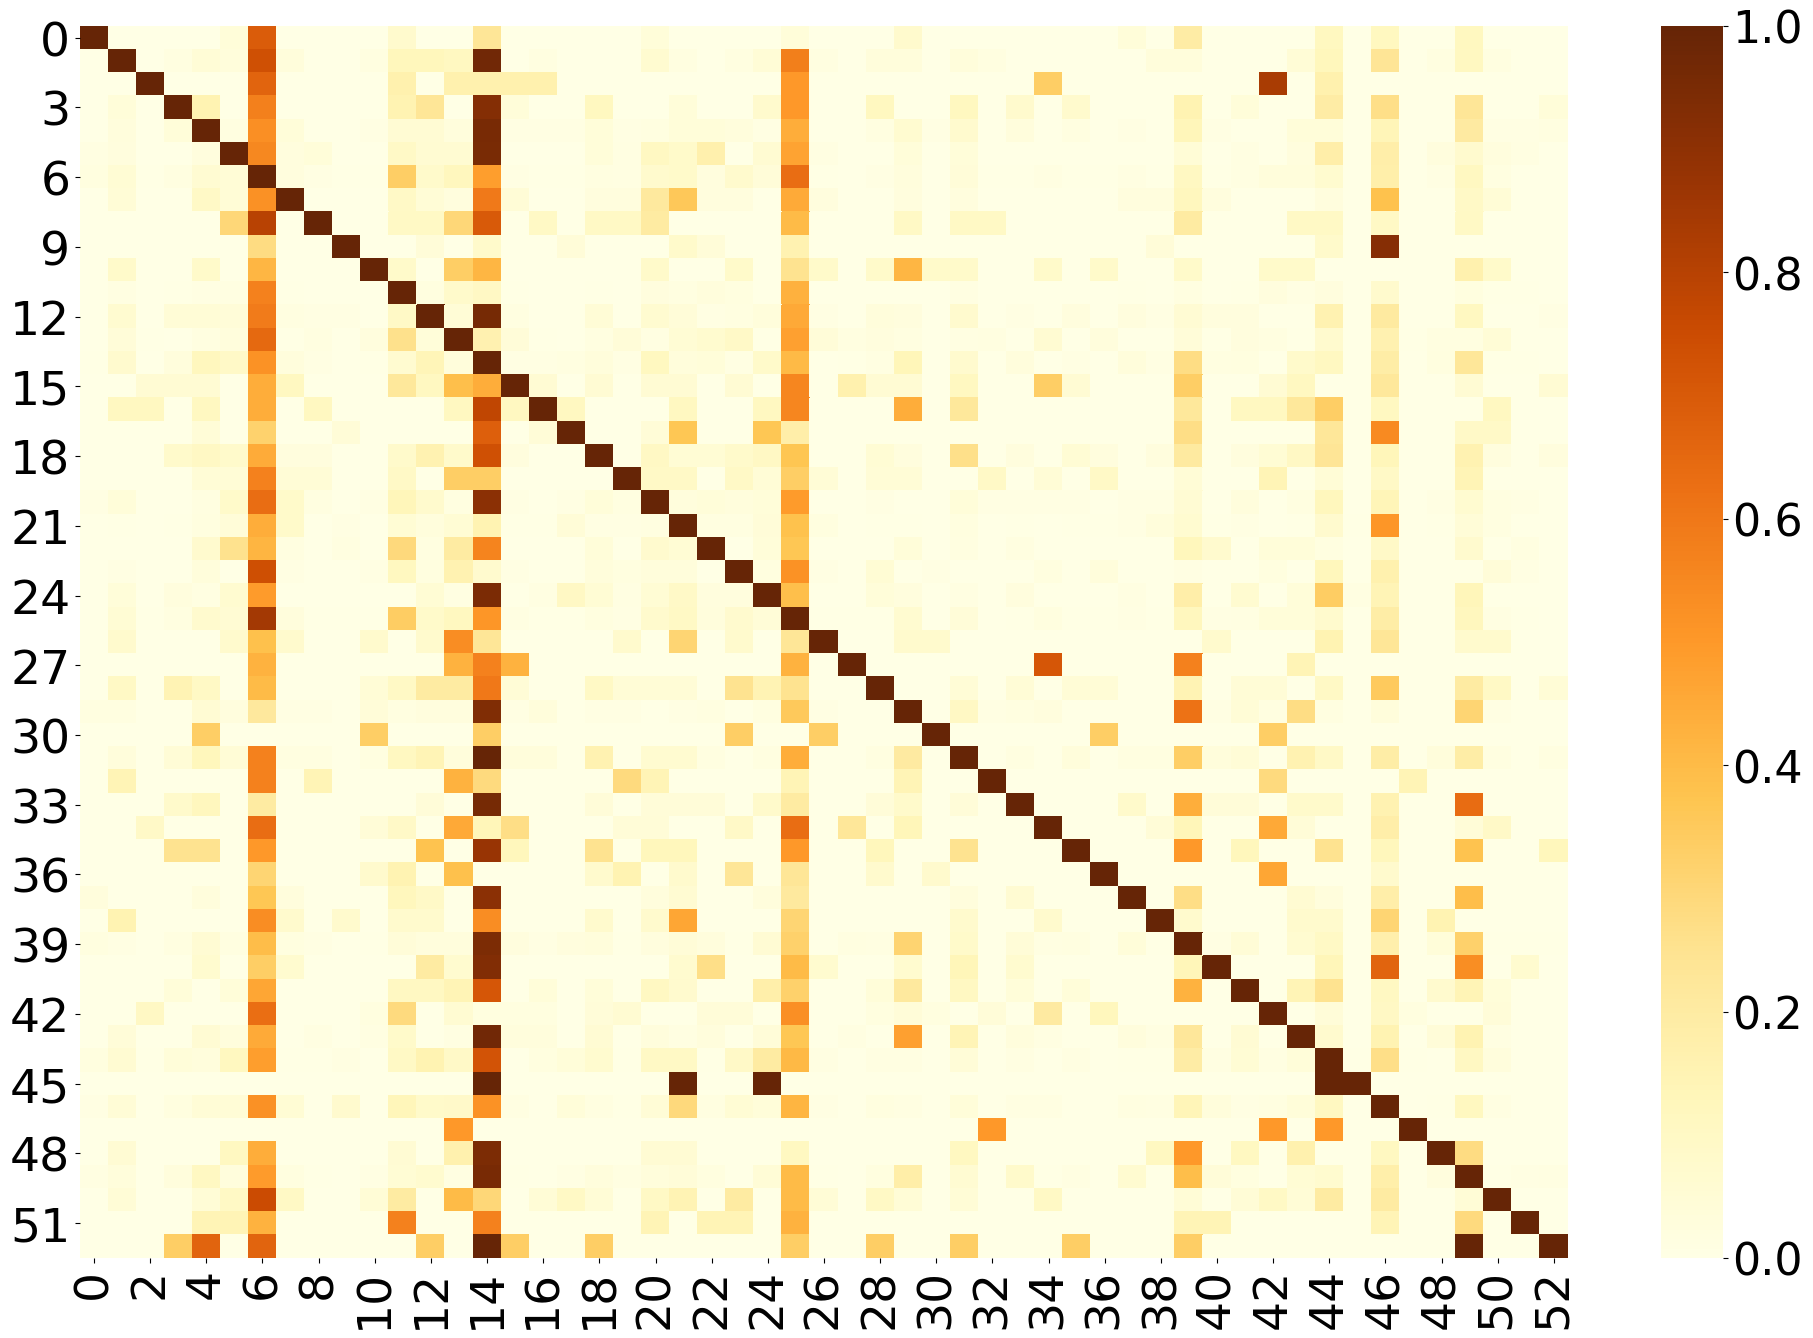
\includegraphics[width=\linewidth / 2]{figures/experiments/syn/enron/enron_relationship_graph.png}
	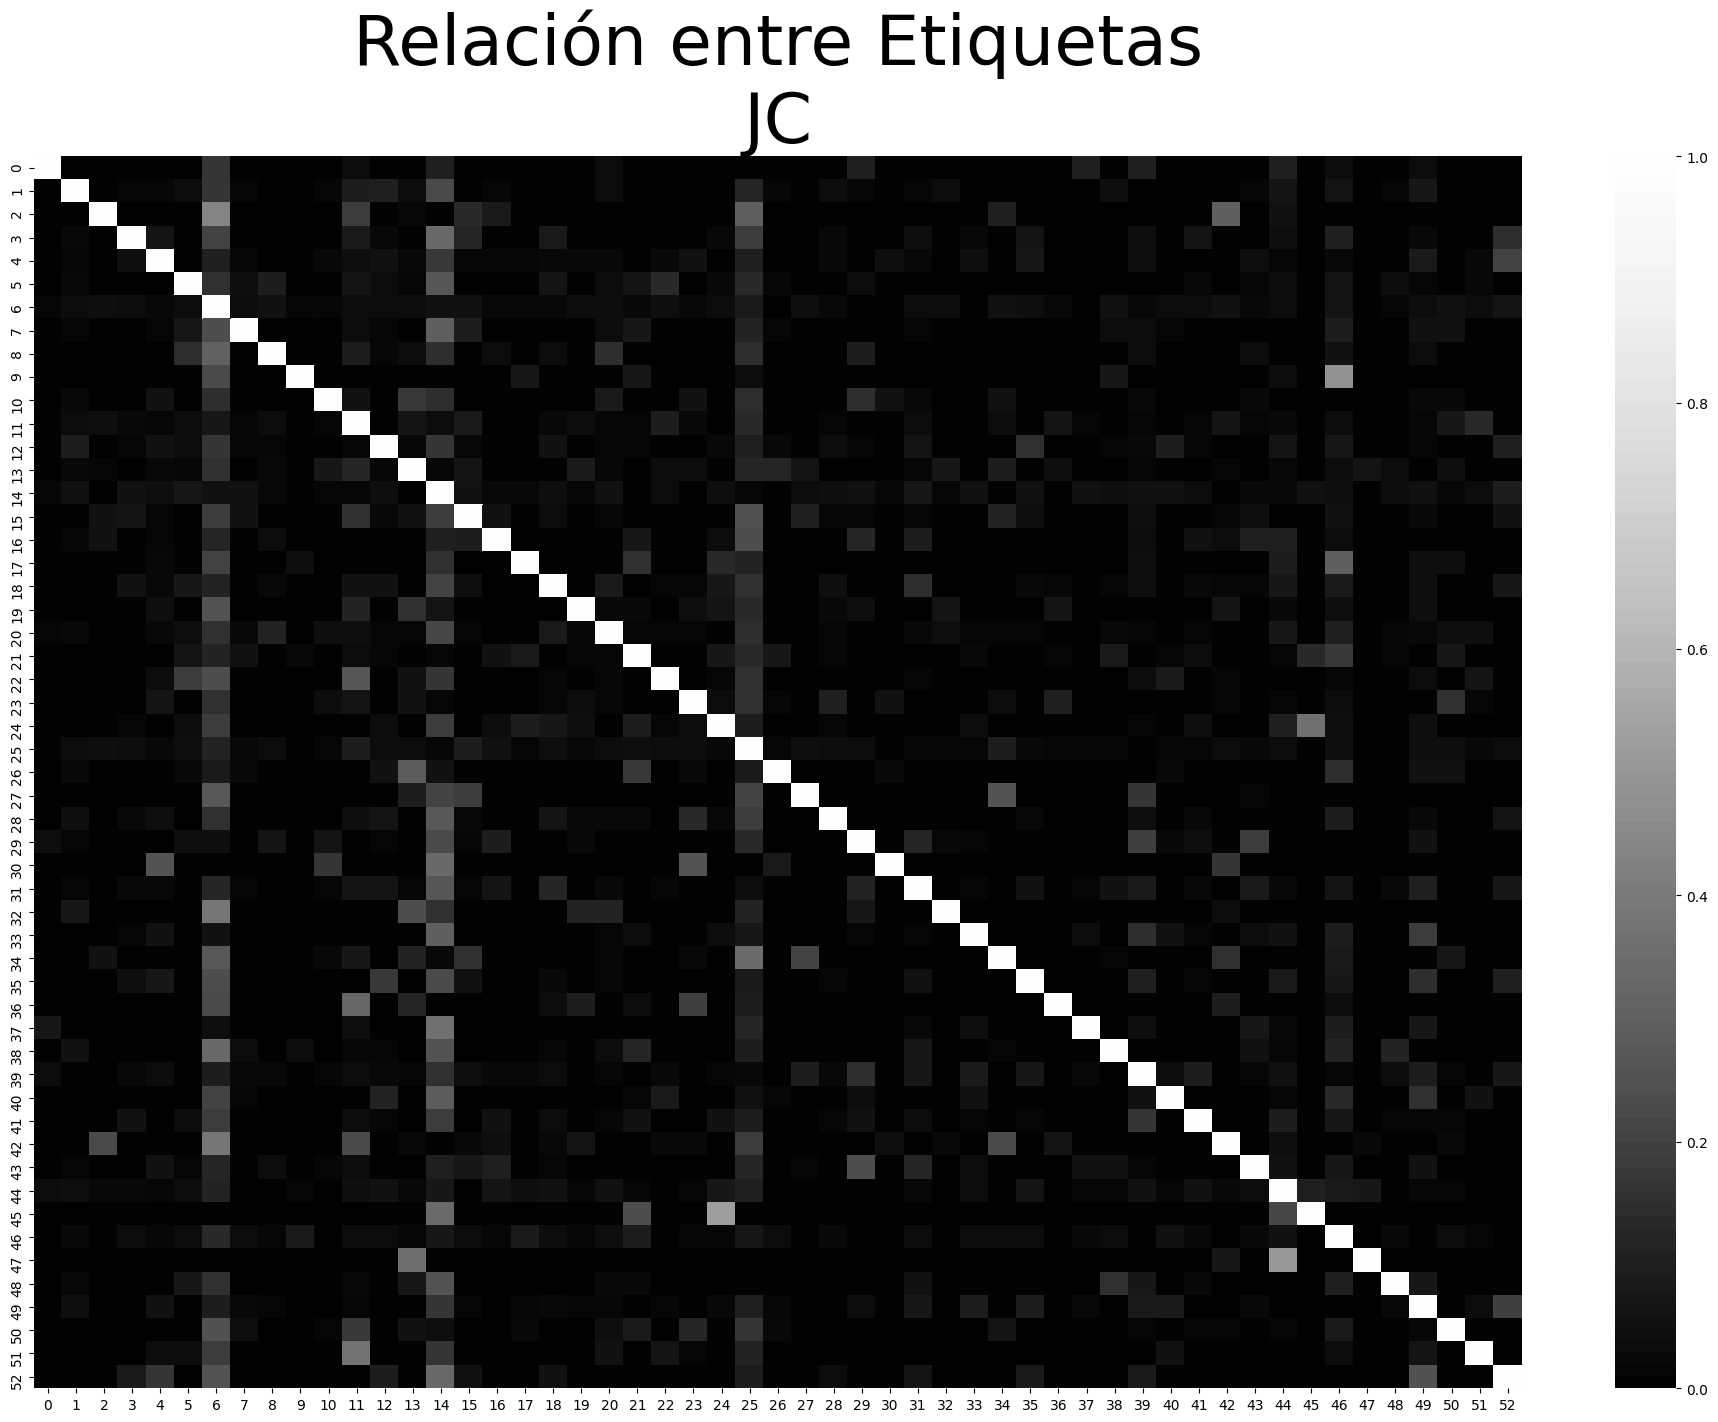
\includegraphics[width=\linewidth /
		2]{figures/experiments/syn/enron/JC_relationship_graph.png}
	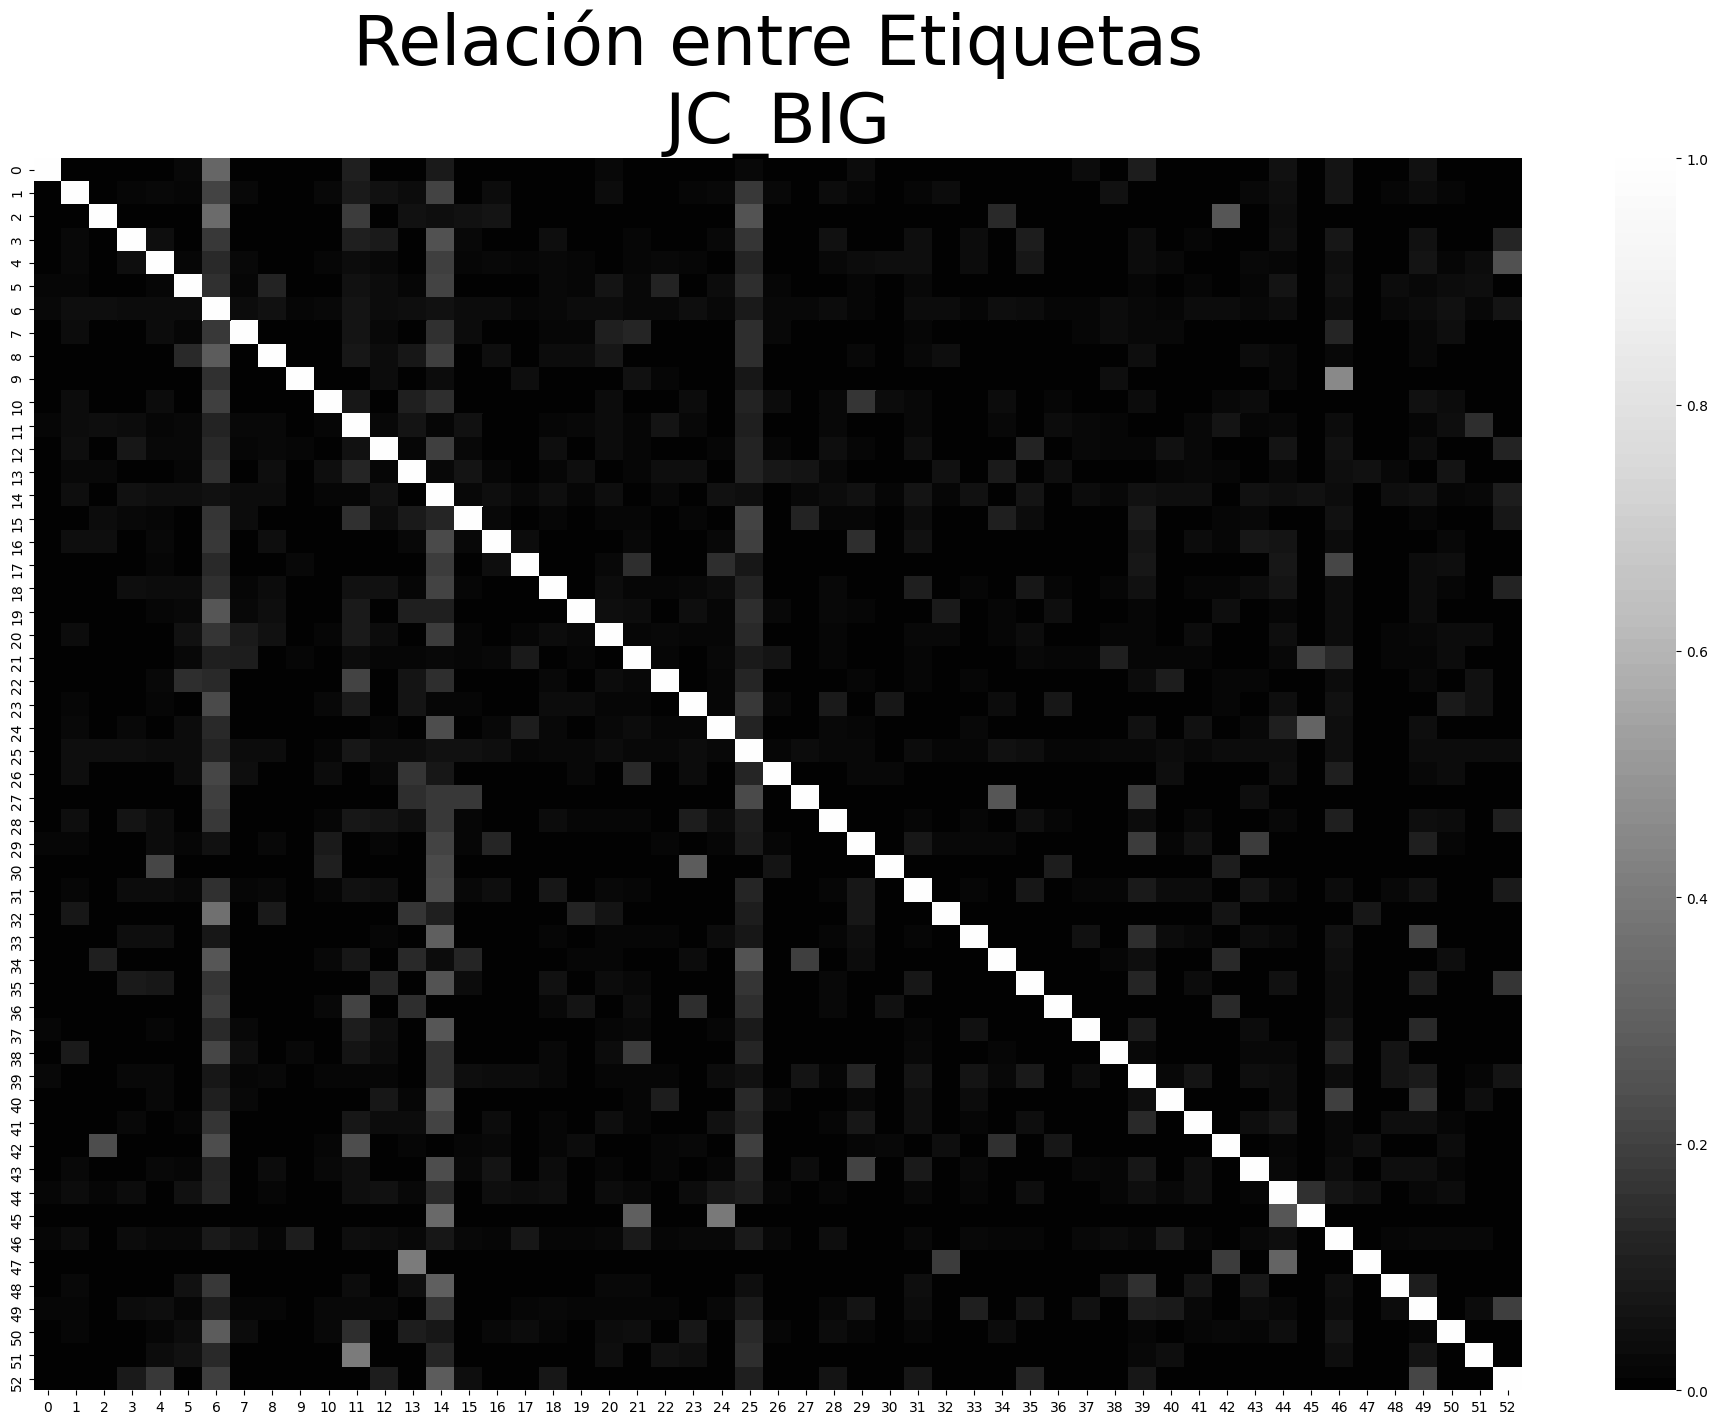
\includegraphics[width=\linewidth /
		2]{figures/experiments/syn/enron/JC_BIG_relationship_graph.png}
	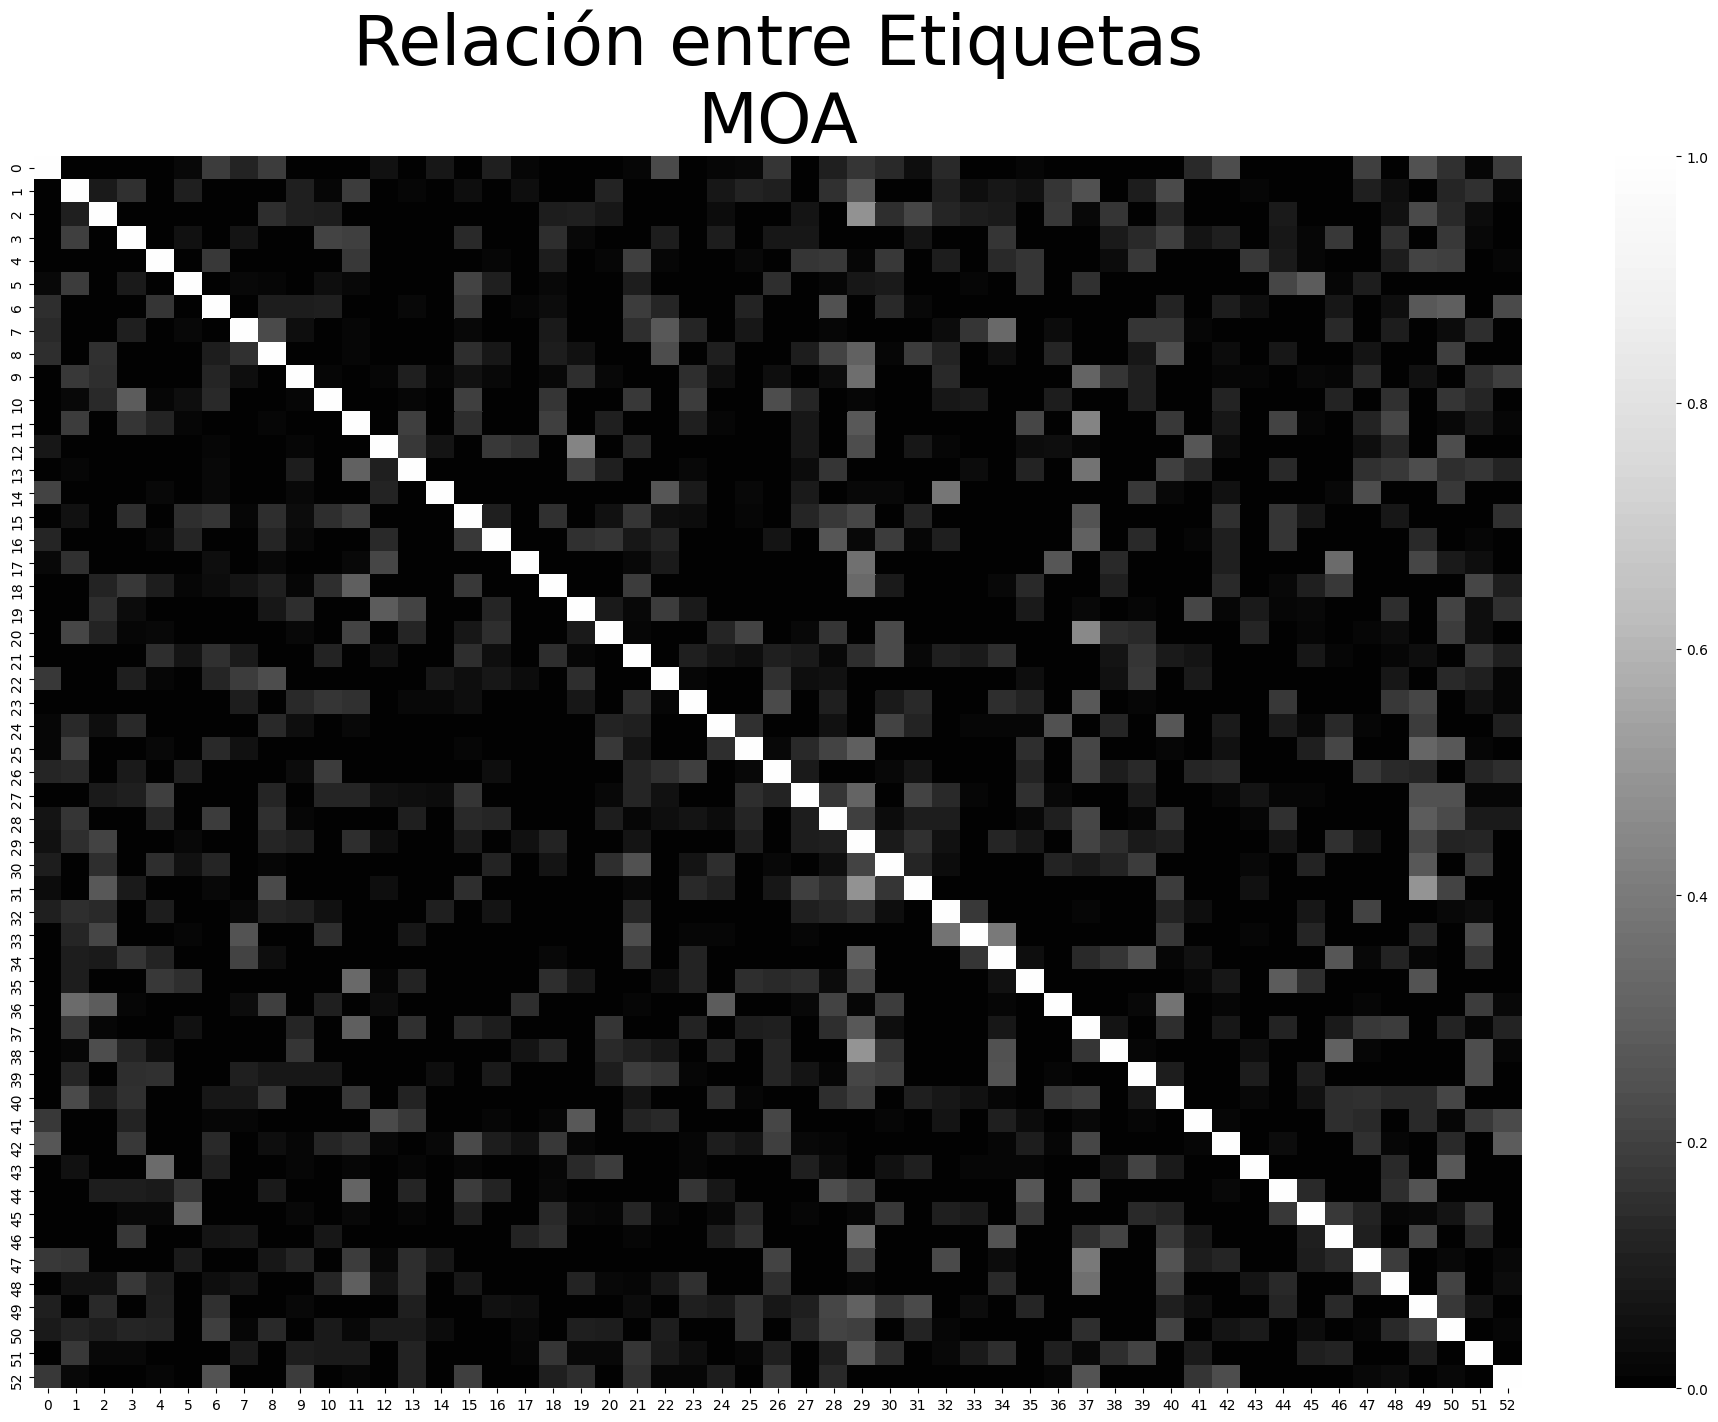
\includegraphics[width=\linewidth /
		2]{figures/experiments/syn/enron/MOA_relationship_graph.png}
	\caption{Relación entre etiquetas para cada \textit{stream} generado sobre
		la colección Enron. Arriba a la izquierda: \textit{Stream} original. Arriba a la
		derecha: \textit{Stream} JC. Abajo a la izquierda: \textit{Stream}
		JC\_BIG. Abajo a la derecha: \textit{Stream} MOA.}
	\label{fig:syn_enron_label_relationship}
\end{figure}

\subsubsection{Mediamill}

\begin{table}[htbp]
	\centering
	\begin{adjustbox}{max width=\textwidth}
		\begin{tabular}{lrrrr}
	\toprule
	\multicolumn{5}{c}{Mediamill}            \\[3pt]
	Nombre    & N      & L   & LC    & LD    \\
	\midrule
	Mediamill & 43907  & 101 & 4,376 & 0,043 \\[3pt]
	MOA       & 43907  & 101 & 4,071 & 0,040 \\[3pt]
	JC        & 43907  & 101 & 2,435 & 0,024 \\[3pt]
	JC\_BIG   & 500000 & 101 & 2,439 & 0,024 \\
	\bottomrule
\end{tabular}

	\end{adjustbox}
	\caption{Características de los \textit{streams} sintéticos generados sobre
		la colección Mediamill.  N: número de instancias; L: número de etiquetas; LC:
		cardinalidad de etiquetas; LD: densidad de etiquetas.}
	\label{tab:syn_mediamill_stats}
\end{table}

La tabla~\ref{tab:syn_mediamill_stats} muestra que el \textit{stream} MOA hace
un buen trabajo en aproximar la cardinalidad de la colección original y presenta
la curva de sesgo más cercana a ella (ver
figura~\ref{fig:syn_mediamill_label_skew}). Se adjunta la
tabla~\ref{tab:syn_20ng_top_labels_combinations} como complemento al estudio del
sesgo.

\begin{figure}[htbp]
	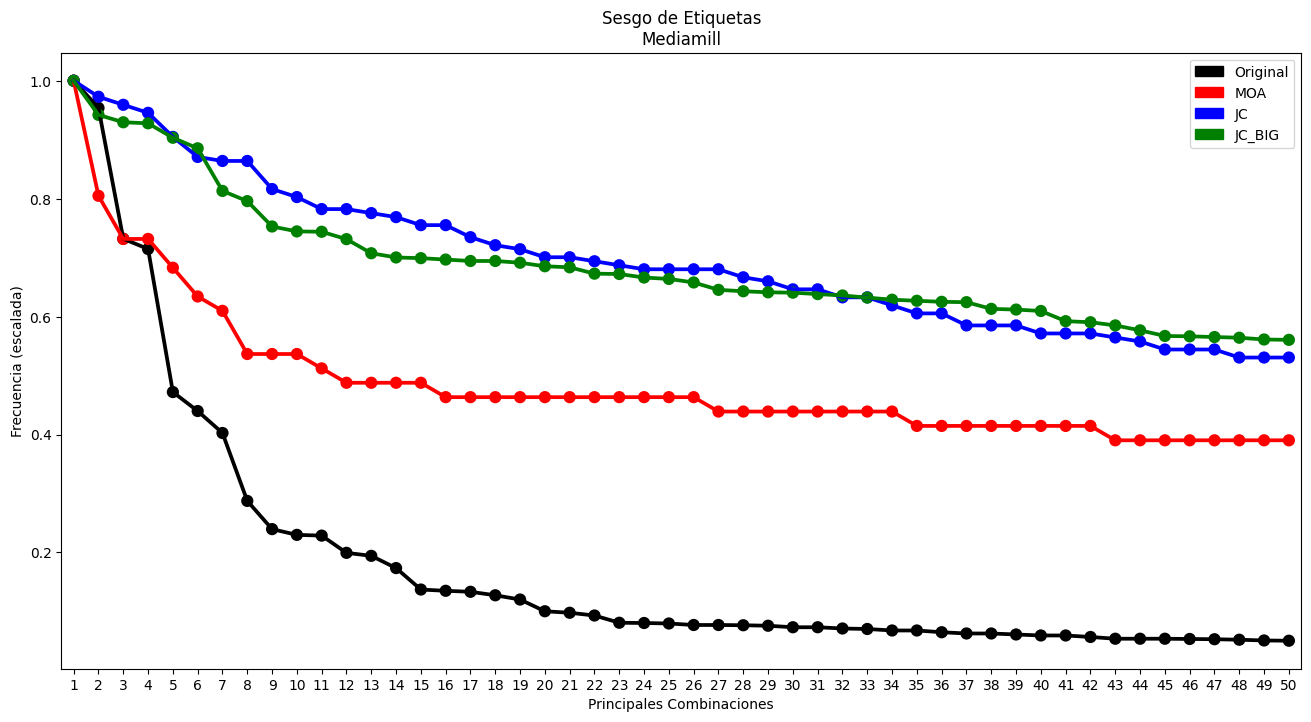
\includegraphics[width=\linewidth]{figures/experiments/syn/mediamill/label_skew.png}
	\caption{Sesgo de etiquetas de los \textit{streams} generados sobre la
		colección Mediamill.}
	\label{fig:syn_mediamill_label_skew}
\end{figure}

\begin{table}[htbp]
	\centering
	\begin{adjustbox}{max width=\textwidth}
		\begin{tabular}{lllll}
	\toprule
	\textit{Rank} & Original                      & JC                            & JC\_BIG                       & MOA                                             \\
	\midrule
	1             & \{Class32, Class34, Class68\} & \{Class48, Class49, Class68\} & \{Class3, Class85\}           & \{Class32, Class38, Class50, Class72\}          \\[3pt]
	2             & \{Class34, Class68\}          & \{Class63, Class85\}          & \{Class31, Class85\}          & \{Class3, Class26, Class89\}                    \\[3pt]
	3             & \{\}                          & \{Class31, Class85\}          & \{Class83, Class85\}          & \{Class18, Class34, Class35, Class89\}          \\[3pt]
	4             & \{Class67\}                   & \{Class3, Class85\}           & \{Class63, Class85\}          & \{Class34, Class35, Class42, Class50, Class73\} \\[3pt]
	5             & \{Class34, Class67, Class68\} & \{Class34, Class78\}          & \{Class32, Class48, Class49\} & \{Class34, Class35, Class42, Class50\}          \\
	\bottomrule
\end{tabular}


	\end{adjustbox}
	\caption{Sesgo de etiquetas - Principales combinaciones de los
		\textit{streams} generados sobre la colección Mediamill.}
	\label{tab:syn_mediamill_top_labels_combinations}
\end{table}

Con respecto a la distribución de etiquetas
(figura~\ref{fig:syn_mediamill_label_distribution}) las conclusiones son
similares a las realizadas a este efecto para Enron. No es posible determinar
con certeza que alguno de los \textit{streams} refleja el fenómeno en mayor
grado que otro, e incluso, si se analiza el gráfico de \textit{mean absolute
	error}, se puede observar que hay 3 puntos donde la curva de JC se aproxima más
al del original y 3 donde el más próximo es MOA. En cuanto al tipo de
distribución, del cual se hace mención en el trabajo de referencia, todos los
\textit{streams} sintéticos obedecen al tipo B, es decir, la mayoría de los
ejemplos tienen una cardinalidad de etiquetas mayor que uno.

\begin{figure}[htbp]
	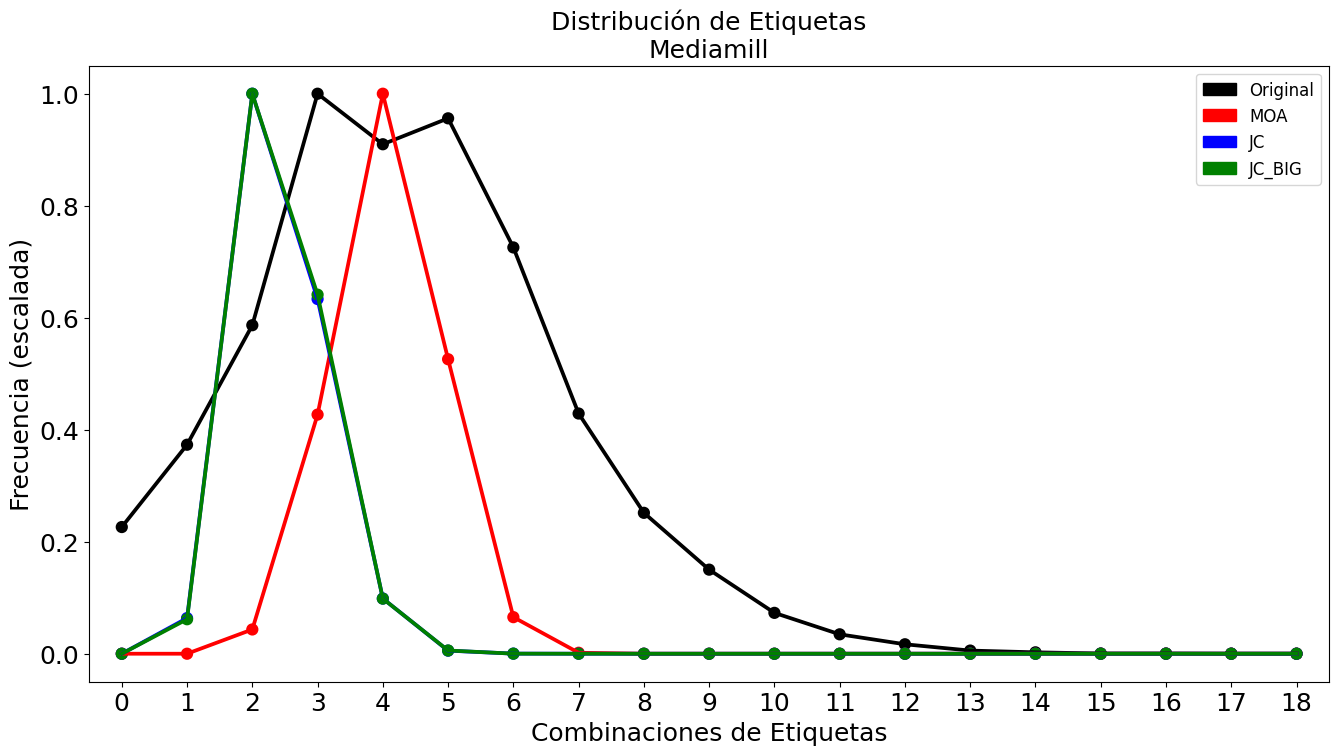
\includegraphics[width=\linewidth]{figures/experiments/syn/mediamill/label_distribution.png}
	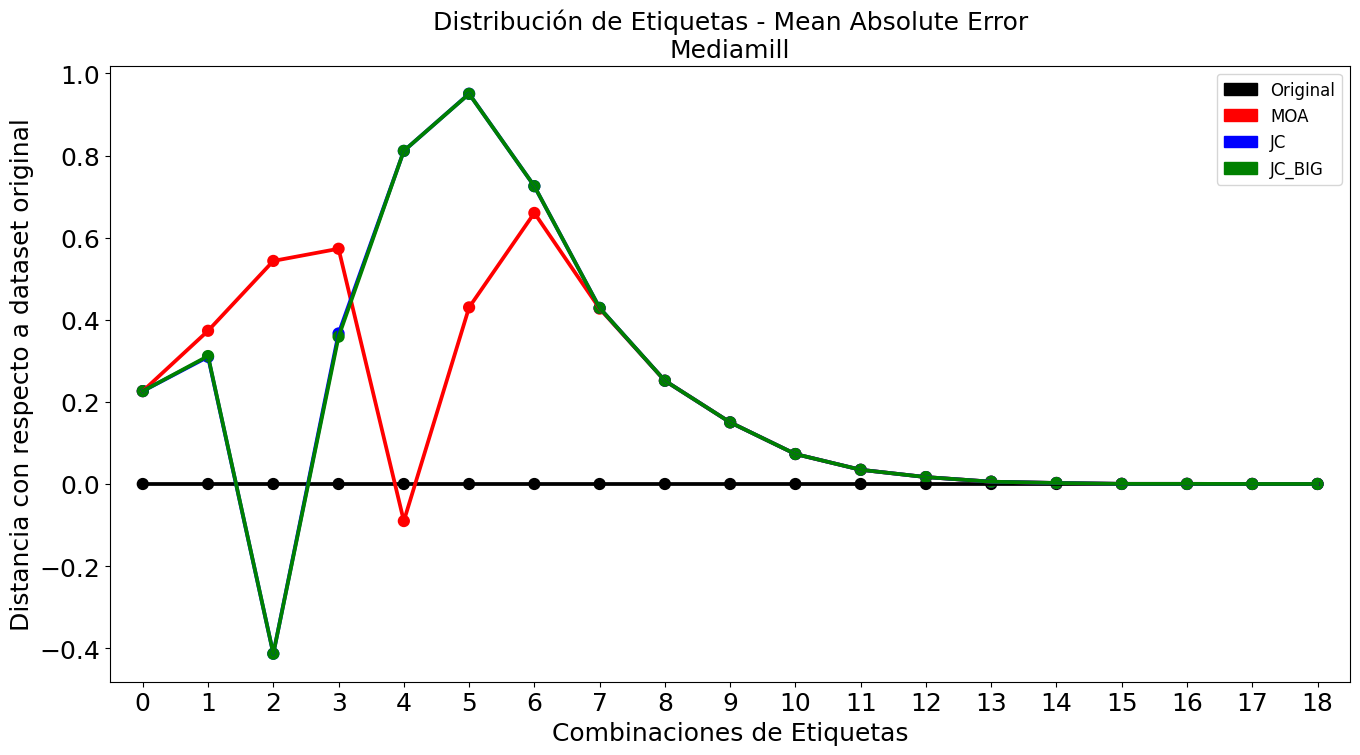
\includegraphics[width=\linewidth]{figures/experiments/syn/mediamill/ld_mae.png}
	\caption{Distribución de etiquetas de los \textit{streams} generados sobre la colección
		Mediamill. Arriba se encuentra el gráfico con las frecuencias escaladas y
		abajo el \textit{mean absolute error} entre cada \textit{stream} y la
		colección original.}
	\label{fig:syn_mediamill_label_distribution}
\end{figure}

También sobre el fenómeno de la dependencia entre etiquetas se pueden hacer
conclusiones similares a las de Enron (ver
figura~\ref{fig:syn_mediamill_label_relationship}). Los gráficos de JC y JC\_BIG
nuevamente reflejan una coloración muy similar al del original, y con una
tonalidad de blanco menos intensa que podría ser producto de un menor valor de
cardinalidad existente en estos \textit{streams} y con respecto al original.

\begin{figure}[htbp]
	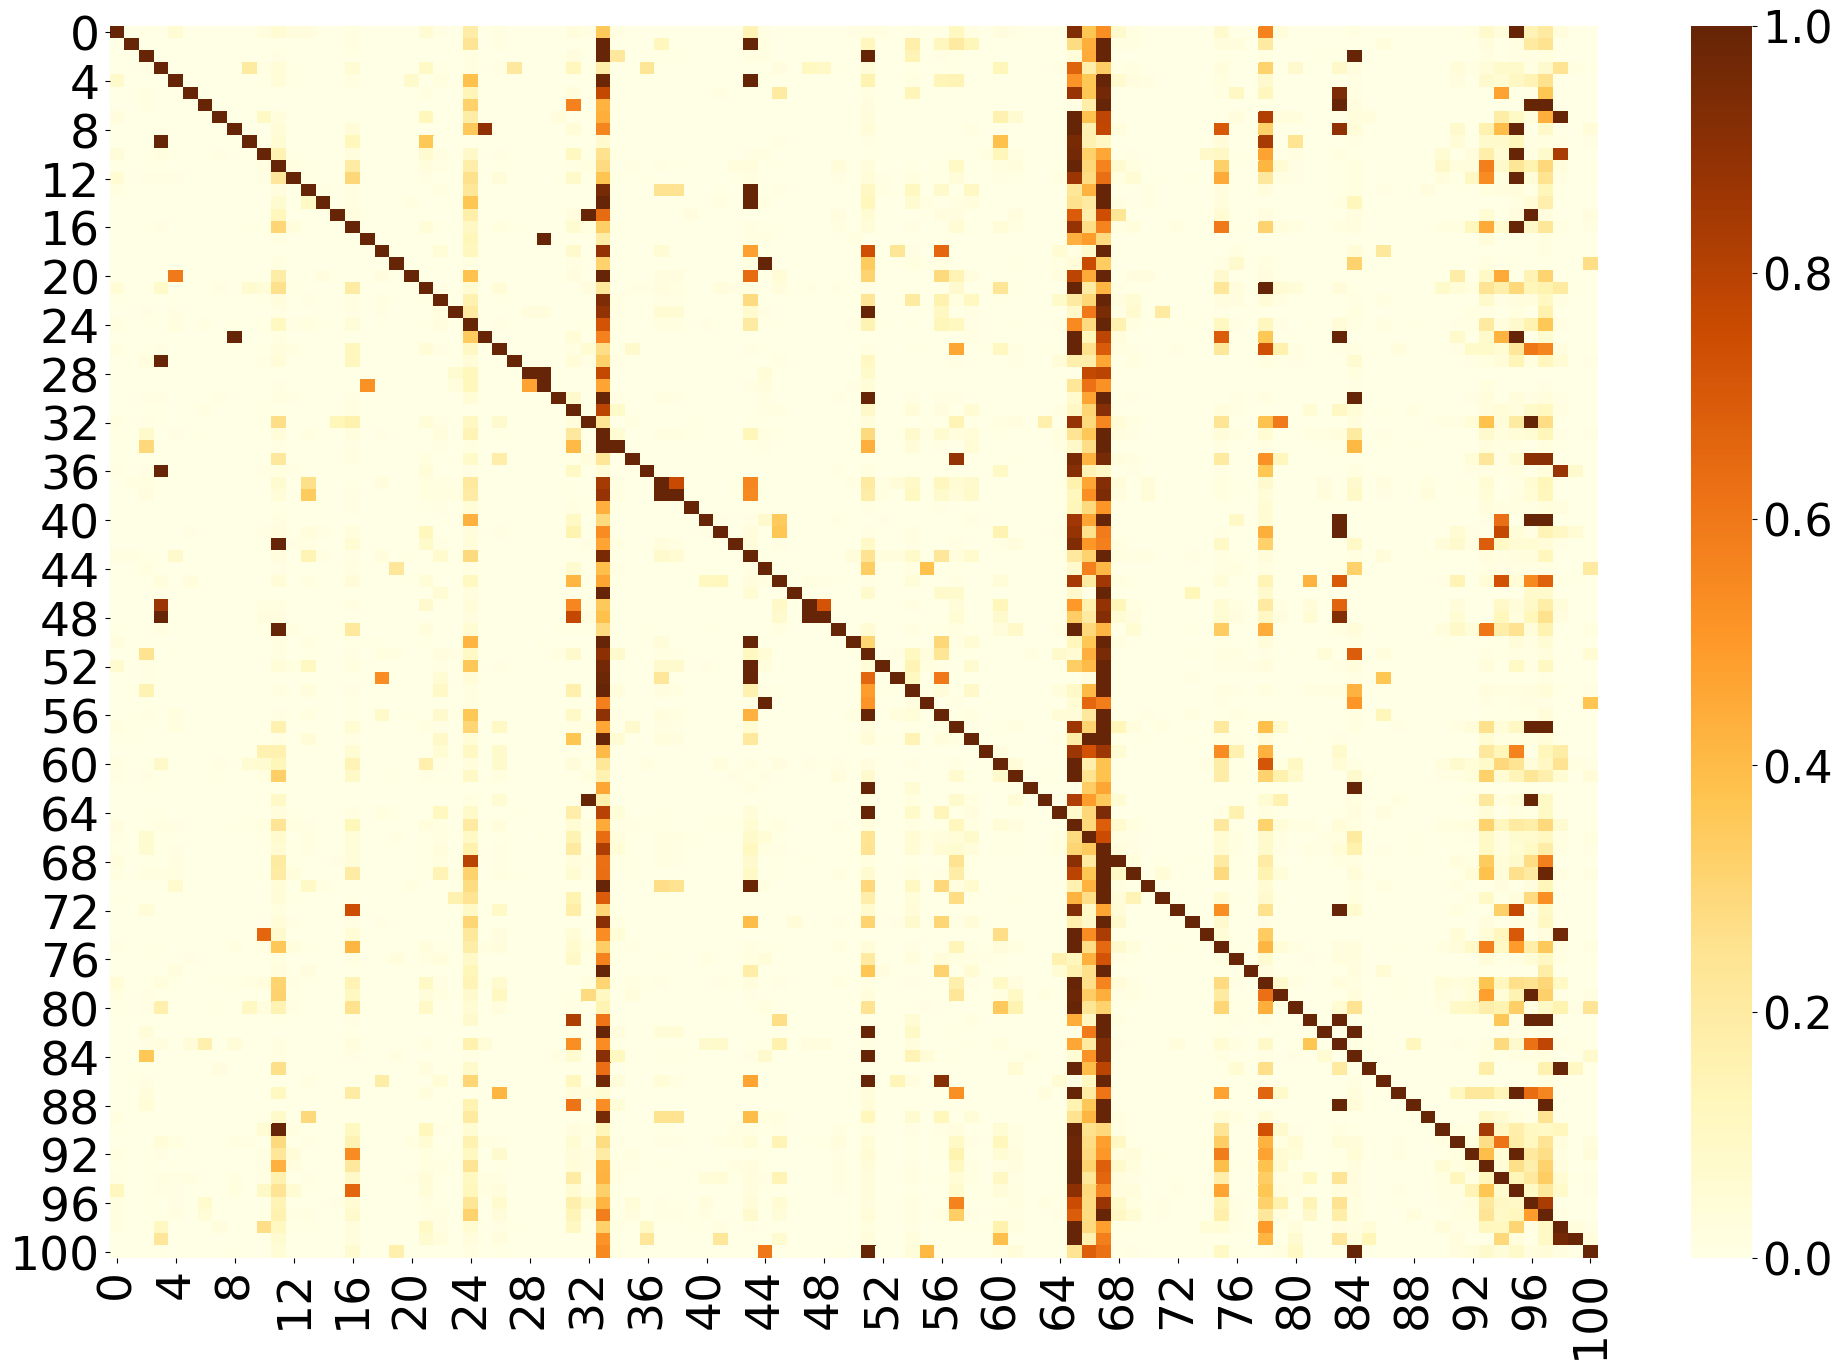
\includegraphics[width=\linewidth /
		2]{figures/experiments/syn/mediamill/mediamill_relationship_graph.png}
	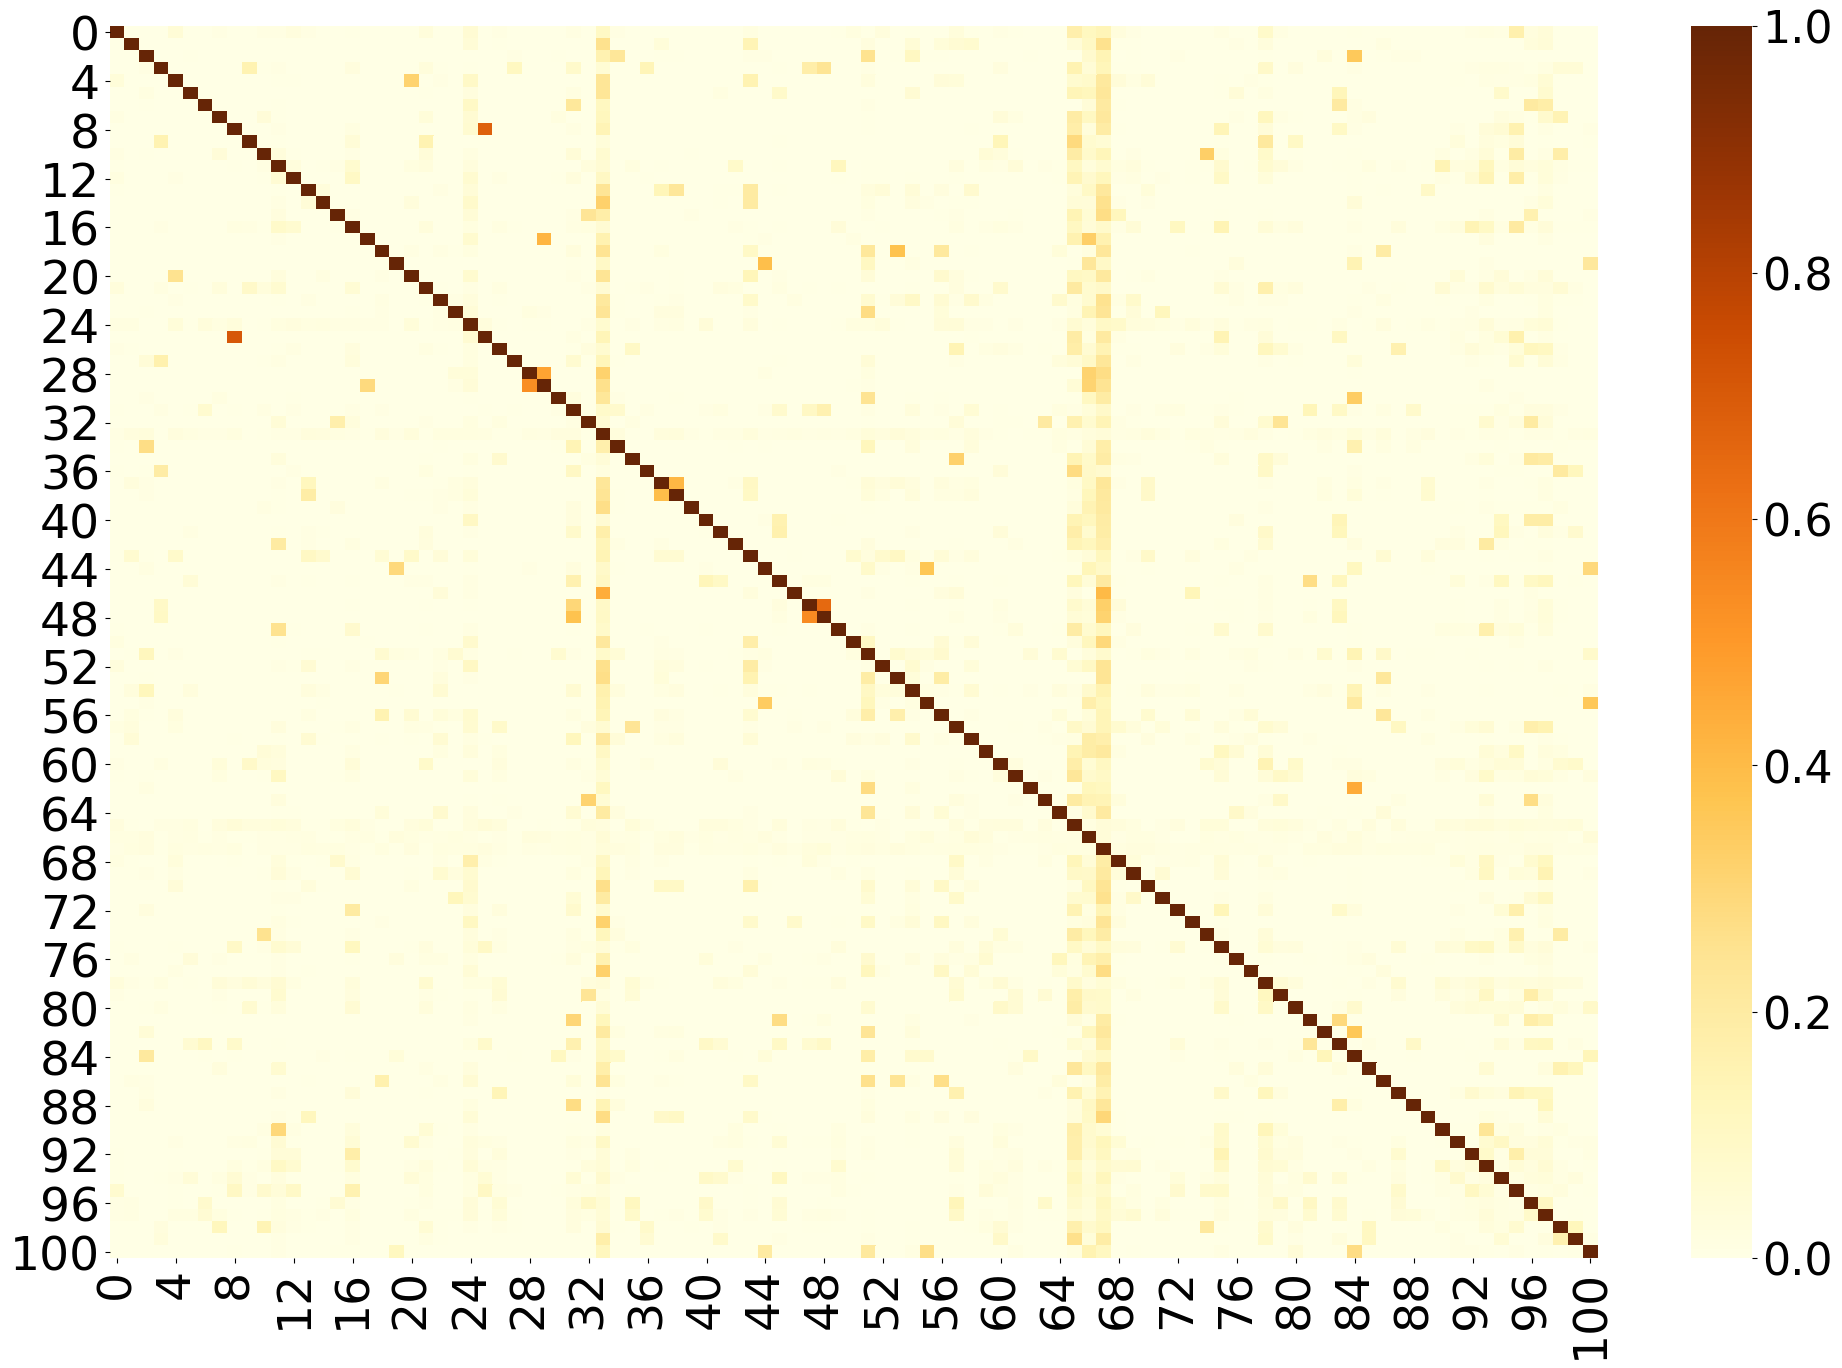
\includegraphics[width=\linewidth /
		2]{figures/experiments/syn/mediamill/JC_relationship_graph.png}
	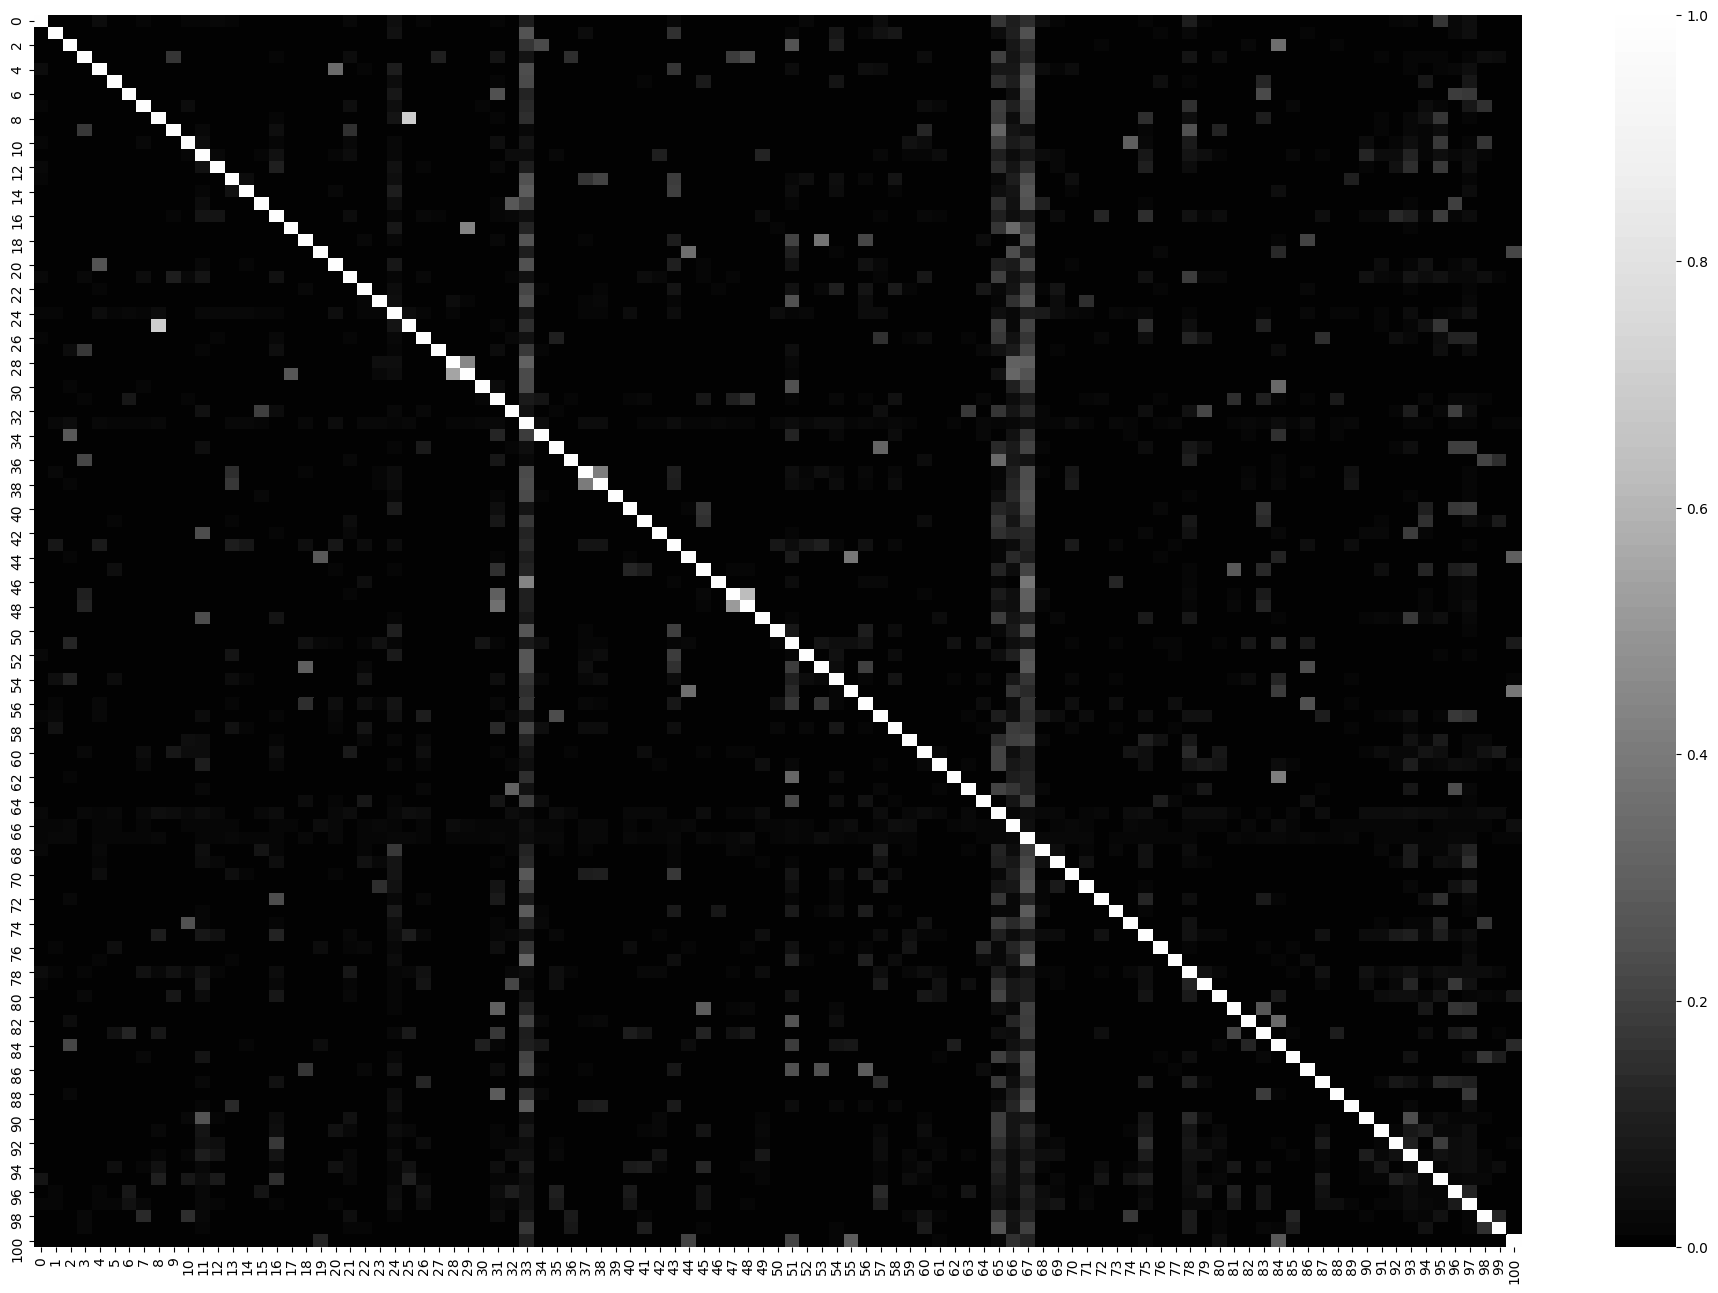
\includegraphics[width=\linewidth /
		2]{figures/experiments/syn/mediamill/JC_BIG_relationship_graph.png}
	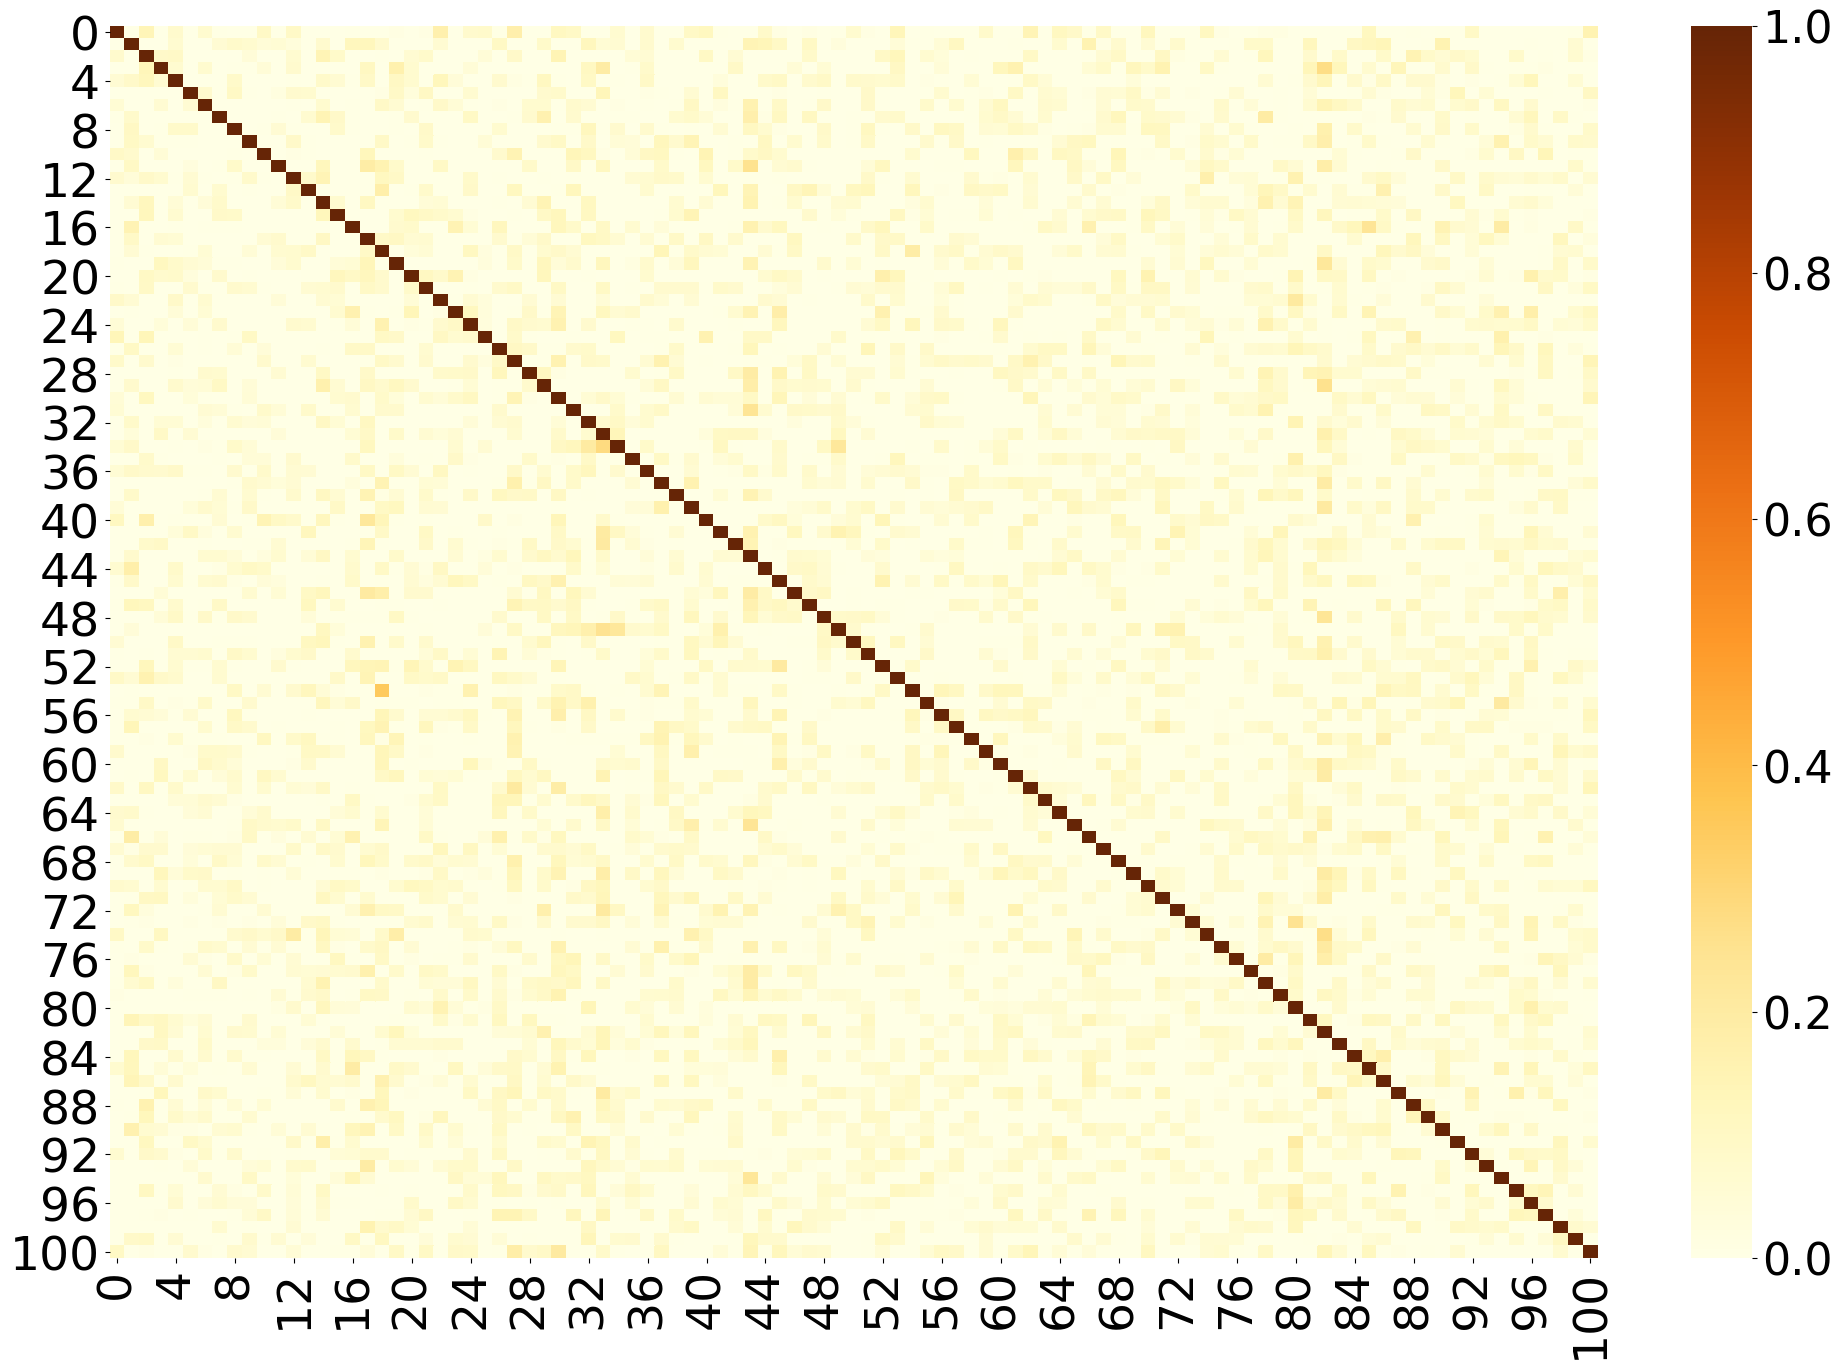
\includegraphics[width=\linewidth /
		2]{figures/experiments/syn/mediamill/MOA_relationship_graph.png}
	\caption{Relación entre etiquetas para cada \textit{stream} generado sobre
		la colección Mediamill. Arriba a la izquierda: \textit{Stream} original.
		Arriba a la derecha: \textit{Stream} JC. Abajo a la izquierda:
		\textit{Stream} JC\_BIG. Abajo a la derecha: \textit{Stream} MOA.}
	\label{fig:syn_mediamill_label_relationship} \end{figure}

\subsection{Clasificaciones}

La metodología propuesta permitió evaluar los diferentes algoritmos de
clasificación multi-etiqueta para los diferentes \textit{streams} utilizando las
configuraciones sin ensambles, los ensambles de referencias y los métodos de
ensamble propuestos. Los resultados se dividen en métricas de ajustes del modelo
basadas en ejemplos (tabla~\ref{tab:example_based}), métricas basadas en
etiquetas (tabla \ref{tab:label_based}), y por último las métricas de eficiencia
(tabla \ref{tab:efficiency}) que cuantifican el tiempo de procesamiento y
espacio de almacenamiento de los modelos. Se marca en negrita la celda
correspondiente al modelo que obtuvo el mejor valor de métrica para la
correspondiente colección de datos. Para cerrar la sección se hace una
comparativa contra experimentos de la literatura de referencia.

\subsubsection{Resultados para Métricas Basadas en Ejemplos}

\begin{table}[htbp]
	\centering
	\begin{adjustbox}{max width=\textwidth}
		\begin{tabular}{l:rrr:rrr:rrr}
	\toprule
	                                            &
	\multicolumn{3}{:c}{\textit{Exact-match}}   &
	\multicolumn{3}{:c}{\textit{Hamming score}} &
	\multicolumn{3}{:c}{\textit{Hamming loss}}                                                                                                     \\
	\textit{Stream}                             & 20ng           & Enron
	                                            & Mediamill      & 20ng           & Enron
	                                            & Mediamill      & 20ng           & Enron          &
	Mediamill                                                                                                                                      \\
	\midrule
	\acrshort{br}                               & 0.228          & 0.018
	                                            & 0.001          & 0.952          & 0.912
	                                            & 0.711          & 0.048
	                                            & \textbf{0.088} & \textbf{0.289}                                                                  \\
	\acrshort{cc}                               & 0.244          & 0.017          & 0.005          & 0.954 & 0.919 & 0.905 & 0.046 & 0.081 & 0.095 \\
	\acrshort{mlht}                             & \textbf{0.315} & \textbf{0.055}
	                                            & \textbf{0.048} & 0.934
	                                            & 0.928          & \textbf{0.957}
	                                            & \textbf{0.066} & 0.072          & 0.043                                                          \\
	\hline
	\acrshort{dwm} (\acrshort{br})              & 0.171          & 0.021
	                                            & 0.001          & \textbf{0.956} & 0.938          & 0.800 & 0.044 & 0.062 & 0.200                 \\
	\acrshort{dwm} (\acrshort{cc})              & 0.167          & 0.024
	                                            & 0.014          & 0.956          & \textbf{0.939} & 0.936 & 0.044 & 0.061 & 0.064                 \\
	\acrshort{ebr}                              & 0.153          & 0.012          & 0.001          & 0.953 & 0.928 & 0.726 & 0.047 & 0.072 & 0.274 \\
	\acrshort{ecc}                              & 0.115          & 0.012          & 0.001          & 0.952 & 0.938 & 0.923 & 0.048 & 0.062 & 0.077 \\
	\hline
	\acrshort{efmp}                             & 0.241          & 0.032          & 0.012          & 0.954 & 0.928 & 0.946 & 0.046 & 0.072 & 0.054 \\
	\acrshort{efmp2}                            & 0.220          & 0.039          & 0.004          & 0.955 & 0.936 & 0.928 & 0.045 & 0.064 & 0.072 \\
	\bottomrule
\end{tabular}

	\end{adjustbox}
	\begin{adjustbox}{max width=\textwidth}
		\begin{tabular}{l:rrr:rrr:rrr:rrr}
	\toprule
	                                        & \multicolumn{3}{:c}{\textit{Accuracy}}     &
	\multicolumn{3}{:c}{\textit{Precision}} &
	\multicolumn{3}{:c}{\textit{Recall}}    & \multicolumn{3}{:c}{\textit{F-score (F1)}}                                                                                                                    \\
	\textit{Stream}                         & 20ng
	                                        & Enron
	                                        & Mediamill                                  & 20ng           & Enron
	                                        & Mediamill                                  & 20ng           & Enron &
	Mediamill                               & 20ng
	                                        & Enron                                      & Mediamill                                                                                                        \\
	\midrule
	\acrshort{br}                           & 0.952
	                                        & 0.912                                      & 0.711          & 0.295
	                                        & 0.326
	                                        & 0.093                                      & \textbf{0.373} &
	\textbf{0.365}                          & \textbf{0.651}
	                                        & \textbf{0.329}                             & 0.345          & 0.163                                                                                           \\
	\acrshort{cc}                           & 0.954                                      & 0.919          & 0.905 & 0.294 & 0.337          & 0.229 & 0.339          & 0.353 & 0.485 & 0.315 & 0.344 & 0.311 \\
	\acrshort{mlht}                         & 0.934
	                                        & 0.928
	                                        & \textbf{0.957}
	                                        & \textbf{0.327}
	                                        & 0.269                                      & \textbf{0.488} &
	0.321                                   & 0.127                                      & 0.378          & 0.324 & 0.172 & \textbf{0.426}                                                                  \\
	\hline
	\acrshort{dwm} (\acrshort{br})          & \textbf{0.956}                             & 0.938          & 0.800 & 0.187 & 0.305          & 0.129 & 0.197          & 0.183 & 0.623 & 0.192 & 0.229 & 0.214 \\
	\acrshort{dwm} (\acrshort{cc})          & 0.956
	                                        & \textbf{0.939}                             & 0.936          & 0.178 & 0.308 & 0.350          & 0.183 & 0.185          & 0.466 & 0.181 & 0.231 & 0.400         \\
	\acrshort{ebr}                          & 0.953                                      & 0.928          & 0.726 & 0.185 & 0.320          & 0.099 & 0.213          & 0.269 & 0.649 & 0.198 & 0.292 & 0.171 \\
	\acrshort{ecc}                          & 0.952                                      & 0.938          & 0.923 & 0.136 & 0.375          & 0.291 & 0.149          & 0.227 & 0.583 & 0.142 & 0.283 & 0.388 \\
	\hline
	\acrshort{efmp}                         & 0.954
	                                        & 0.928                                      & 0.946          &
	0.302                                   & 0.380                                      & 0.404          & 0.361 & 0.351 & 0.418          & 0.328 & \textbf{0.365} & 0.411                                 \\
	\acrshort{efmp2}                        & 0.955
	                                        & 0.936                                      & 0.928          & 0.252 &
	\textbf{0.389}                          & 0.303                                      & 0.277          & 0.303 & 0.516 & 0.264          & 0.340 & 0.382                                                  \\
	\bottomrule
\end{tabular}

	\end{adjustbox}
	\caption{Resultados de métricas basadas en ejemplos sobre los
		\textit{streams} seleccionados para cada algoritmo evaluado.}
	\label{tab:example_based}
\end{table}

\begin{figure}
	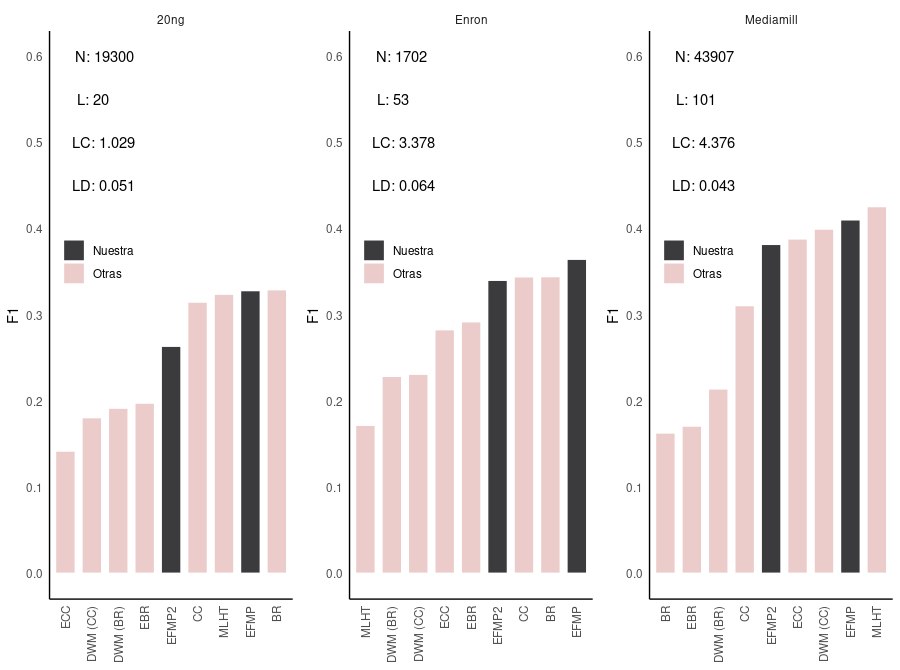
\includegraphics[width=\linewidth,height=10cm]{figures/experiments/classification/f1_ex.png}
	\caption{Comparativa de modelos bajo la métrica \textit{f1} basada en
		ejemplos.}
	\label{fig:comparativa_f1_ex}
\end{figure}

Los valores de F1 obtenidos para la evaluación basada en ejemplos (Tabla
\ref{tab:example_based}) muestra que \acrshort{efmp} y \acrshort{efmp2} fueron
mejores que los \textit{baselines} de ensambles en todos los casos.  Además,
superó a los que no utilizan ensambles en el \textit{stream} de Enron.  En los
casos de 20ng, \acrshort{efmp} fue superado en un 0.001\% por \acrshort{br} y en
Mediamill \acrshort{mlht} superó a \acrshort{efmp} en un 0.015\%. Para el caso
de \textit{exact-match} el modelo dominante es \acrshort{mlht}, lo cual es un
resultado en consonancia con otros estudios de la
literatura~\cite{read_scalable_2012,osojnik_multi-label_2017,zheng_survey_2020},
y los modelos propuestos se ubican en segundo lugar para dos de las tres
colecciones. En cuanto al \textit{hamming score} los resultados son muy
similares entre colecciones de datos, con los modelos de \acrshort{dwm} sacando
una leve ventaja para 20ng y Enron pero siendo superado por \acrshort{efmp} y
\acrshort{mlht} para Mediamill. También se observan resultados competitivos en
la métrica de \textit{accuracy} donde \acrshort{efmp} supera a todos los modelos
para Enron, incluyendo al de \acrshort{mlht} que es el dominante para Mediamill
y 20ng.

La figura~\ref{fig:comparativa_f1_ex} muestra la comparativa de rendimientos
entre modelos bajo la métrica de \textit{f1}, ordenados desde el menos
performante al más performante y con los modelos aquí presentados en color
negro. Se puede observar cómo en cada \textit{stream} el modelo \acrshort{efmp}
se sitúa entre los dos mejores, siendo el de mejor rendimiento para Enron. De
manera similar, \acrshort{efmp2} se sitúa en cuarto puesto para Enron y quinto
para los demás. Es de notar que otros modelos no logran emparejar rendimientos
entre \textit{streams}, véase el caso de \acrshort{mlht} por ejemplo, que es el
mejor para Mediamill pero cae en el último puesto para Enron. Este resultado es
coherente con la idea de que los modelos derivados de \acrlong{ht} requieren de
un mayor número de instancias para identificar el mejor punto de corte de un
nodo y lograr mejores evaluaciones~\cite{read_scalable_2012}. Algo similar
sucede con los dos modelos de \acrshort{dwm} que logran valores altos para
Mediamill pero se ubican entre los tres menos performantes para Enron y 20ng.

\subsubsection{Resultados para Métricas Basadas en Etiquetas}

\begin{table}[htbp]
	\centering
	\begin{adjustbox}{max width=\textwidth}
		\begin{tabular}{lrrrrrrrrr}
	\toprule
	                & \multicolumn{3}{l}{macro\_precision} & \multicolumn{3}{l}{macro\_recall} & \multicolumn{3}{l}{macro\_fscore}                                                         \\
	stream          & 20ng                                 & enron                             & mediamill                         & 20ng  & enron & mediamill & 20ng  & enron & mediamill \\
	\midrule
	br\_nb          & 0.604                                & 0.106                             & 0.062                             & 0.373 & 0.110 & 0.553     & 0.461 & 0.108 & 0.111     \\
	cc\_nb          & 0.667                                & 0.113                             & 0.065                             & 0.340 & 0.097 & 0.150     & 0.450 & 0.105 & 0.091     \\
	dwmc\_br        & 0.781                                & 0.121                             & 0.064                             & 0.196 & 0.031 & 0.418     & 0.314 & 0.049 & 0.111     \\
	dwmc\_cc        & 0.814                                & 0.114                             & 0.068                             & 0.183 & 0.030 & 0.111     & 0.299 & 0.047 & 0.084     \\
	lcht            & 0.546                                & 0.005                             & 0.074                             & 0.318 & 0.016 & 0.030     & 0.402 & 0.008 & 0.043     \\
	me2\_lcht       & 0.699                                & 0.143                             & 0.096                             & 0.276 & 0.059 & 0.173     & 0.396 & 0.083 & 0.124     \\
	me\_lcht        & 0.649                                & 0.114                             & 0.074                             & 0.361 & 0.082 & 0.072     & 0.464 & 0.096 & 0.073     \\
	oza\_ml\_br\_nb & 0.687                                & 0.100                             & 0.062                             & 0.214 & 0.068 & 0.531     & 0.326 & 0.081 & 0.111     \\
	oza\_ml\_cc\_nb & 0.753                                & 0.119                             & 0.049                             & 0.150 & 0.046 & 0.112     & 0.250 & 0.067 & 0.068     \\
	\bottomrule
\end{tabular}

	\end{adjustbox}
	\begin{adjustbox}{max width=\textwidth}
		\begin{tabular}{l:rrr:rrr:rrr}
	\toprule
	                                                &
	\multicolumn{3}{:c}{\textit{Precision} (micro)} &
	\multicolumn{3}{:c}{\textit{Recall} (micro)}    &
	\multicolumn{3}{:c}{\textit{F-score} (micro)}                                                                                                 \\
	\textit{Stream}                                 & 20ng
	                                                & Enron          & Mediamill      & 20ng  &
	Enron                                           & Mediamill      & 20ng           & Enron & Mediamill                                         \\
	\midrule
	\acrshort{br}                                   & 0.552          & 0.330
	                                                & 0.096          &
	\textbf{0.373}                                  & \textbf{0.364} & \textbf{0.673} & 0.445 & 0.347     & 0.168                                 \\
	\acrshort{cc}                                   & 0.597          & 0.364          & 0.224 & 0.340     & 0.353 & 0.485 & 0.433 & 0.358 & 0.306 \\
	\acrshort{mlht}                                 & 0.345          & 0.283
	                                                & \textbf{0.509} & 0.318
	                                                & 0.079          & 0.342          & 0.331
	                                                & 0.124          & \textbf{0.410}                                                             \\
	\hline
	\acrshort{dwm} (\acrshort{br})                  & 0.773          & 0.552          & 0.131 & 0.197     & 0.178 & 0.642 & 0.313 & 0.269 & 0.218 \\
	\acrshort{dwm} (\acrshort{cc})                  & \textbf{0.796} & \textbf{0.569} & 0.328 & 0.183     & 0.179 & 0.463 & 0.298 & 0.272 & 0.384 \\
	\acrshort{ebr}                                  & 0.633          & 0.412          & 0.101 & 0.214     & 0.285 & 0.671 & 0.320 & 0.337 & 0.175 \\
	\acrshort{ecc}                                  & 0.644          & 0.534          & 0.299 & 0.150     & 0.242 & 0.579 & 0.243 & 0.333 & 0.395 \\
	\hline
	\acrshort{efmp}                                 & 0.586          & 0.417
	                                                & 0.384          & 0.361          & 0.339
	                                                & 0.403          &
	\textbf{0.447}                                  & \textbf{0.374} & 0.393                                                                      \\
	\acrshort{efmp2}                                & 0.644          & 0.498          & 0.305 & 0.276     & 0.293 & 0.511 & 0.387 & 0.369 & 0.382 \\
	\bottomrule
\end{tabular}

	\end{adjustbox}
	\caption{Resultados de métricas basadas en etiquetas sobre los
		\textit{streams} seleccionados para cada algoritmo evaluado.}
	\label{tab:label_based}
\end{table}

\begin{figure}
	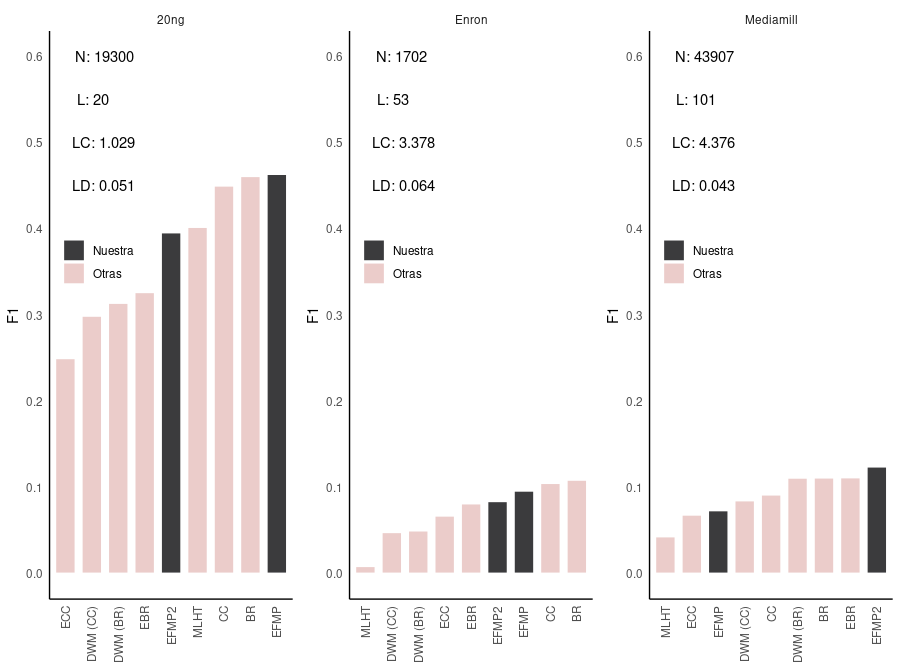
\includegraphics[width=\linewidth,height=10cm]{figures/experiments/classification/f1_macro.png}
	\caption{Comparativa de modelos bajo la métrica \textit{f1} con promedio
		macro, basada en etiquetas.}
	\label{fig:comparativa_f1_macro}
\end{figure}

\begin{figure}
	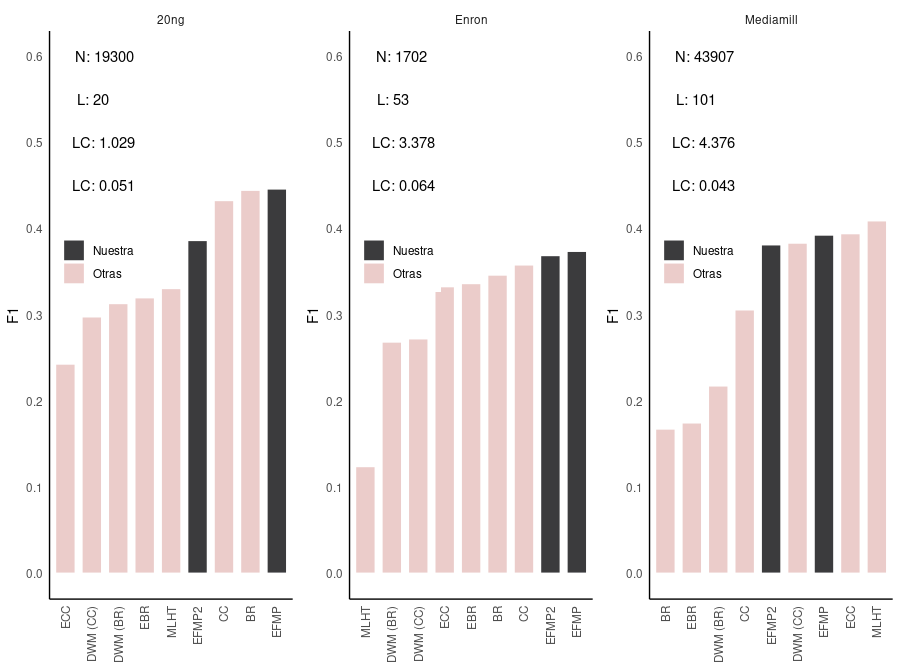
\includegraphics[width=\linewidth,height=10cm]{figures/experiments/classification/f1_micro.png}
	\caption{Comparativa de modelos bajo la métrica \textit{f1} con promedio
		micro, basada en etiquetas.}
	\label{fig:comparativa_f1_micro}
\end{figure}

La métrica de \textit{f1} macro muestra resultados favorecedores para los
modelos presentados. \acrshort{efmp2} obtuvo un valor superior para Mediamill y
\acrshort{efmp} fue el mejor para 20ng y el segundo mejor para Enron, por
centésimas de diferencia con respecto al modelo \acrshort{br}. En lo que
respecta a la comparativa entre soluciones de ensambles, \acrshort{efmp} y
\acrshort{efmp2} superan a las demás para todas las colecciones evaluadas.  Con
relación a los modelos de \acrshort{dwm}, estos muestran una disparidad entre
los valores de precisión y \textit{recall}. Véase por ejemplo el caso de
\acrshort{dwm} (\acrshort{cc}) para 20ng, donde logra más de un 0.8 de precisión
(mejor clasificador) pero un \textit{recall} por debajo de 0.2 (segundo peor
clasificador). Mismo caso pero a la inversa con \acrshort{dwm} (\acrshort{br})
para Mediamill, el cual consigue alrededor de 0.4 de \textit{recall} (tercer
mejor clasificador) pero apenas un 0.06 de precisión (tercer peor
clasificador).  Esta disparidad logra suavizarse en los modelos de
\acrshort{efmp} presentados y se ve reflejado en valores más altos de
\textit{f1}.

También son favorecedores los valores de las métricas de \textit{f1} micro para
los modelos presentados. \acrshort{efmp} es el mejor para las colecciones 20ng y
Enron y es apenas superado por \acrshort{mlht} para el \textit{stream} de
Mediamill. En la comparativa de métodos de ensambles, \acrshort{efmp} es el
mejor modelo para todos las métricas a excepción del caso de \textit{recall}
para Mediamill (donde \acrshort{ebr} obtiene el mejor valor), y los casos de
precisión para Enron y 20ng, donde \acrshort{dwm} (\acrshort{cc}) logra una
clara diferencia. Al respecto de este último modelo se puede hacer las mismas
consideraciones en cuanto a la disparidad entre precisión y \textit{recall}.

Las figuras~\ref{fig:comparativa_f1_macro} y~\ref{fig:comparativa_f1_micro}
muestra la comparativa de rendimientos entre modelos bajo las métricas de
\textit{f1} macro y micro, respectivamente, y con los mejores modelos
posicionados más a la derecha. Para la métrica macro-promediada se puede
observar que al menos uno de los dos modelos de \acrshort{efmp} se posiciona
entre los mejores tres para cada colección y como el mejor método de ensambles.
Lo mismo sucede con la métrica micro-promediada, donde \acrshort{efmp} supera a
los métodos de \acrshort{br} y \acrshort{cc} para 20ng y Enron y queda por
debajo de \acrshort{mlht} y \acrshort{ecc} para Mediamill.

\subsubsection{Resultados para Métricas de Eficiencia}

\begin{table}[htbp]
	\centering
	\begin{adjustbox}{max width=\textwidth}
		\begin{tabular}{l:ccc:ccc}
	\toprule
	                               & \multicolumn{3}{:c}{Tamaño del modelo (kb)} &
	\multicolumn{3}{:c}{Tiempo de ejecución (segundos)}                                                                              \\
	\textit{Stream}                & 20ng                                        & Enron &
	Mediamill                      & 20ng                                        & Enron & Mediamill                                 \\
	\midrule
	\acrshort{br}                  & 31.6
	                               & \textbf{82.9}
	                               & \textbf{18.9}
	                               & \textbf{1:43:26}
	                               & \textbf{0:21:28}
	                               & \textbf{2:08:42}                                                                                \\
	\acrshort{cc}                  & 31.9                                        & 85.1  & 26.7      & 1:45:00  & 0:27:05 & 2:52:36  \\
	\acrshort{mlht}                & \textbf{22.8}                               & 284.7 & 306.0     & 2:22:30  & 0:58:16 & 19:05:49 \\
	\hline
	\acrshort{dwm} (\acrshort{br}) & 305.5
	                               & 782.9                                       & 185.3 & 21:23:37  & 5:15:03  & 1
	día, 4:21:27                                                                                                                     \\
	\acrshort{dwm} (\acrshort{cc}) & 308.4
	                               & 802.7                                       & 262.4 & 21:03:02  & 5:05:56
	                               & 1 día, 12:49:14                                                                                 \\
	\acrshort{ebr}                 & 316.1                                       & 826.8 & 189.2     & 14:14:56 & 3:41:00 & 20:13:01 \\
	\acrshort{ecc}                 & 319.0
	                               & 847.6                                       & 267.2 & 14:35:33  & 4:03:16
	                               & 1 día, 1:23:01                                                                                  \\
	\hline
	\acrshort{efmp}                & 86.4
	                               & 452.8                                       & 351.7 & 5:41:58   & 1:45:51
	                               & 1 día, 0:47:17                                                                                  \\
	\acrshort{efmp2}               & 84.7
	                               & 359.2                                       & 262.2 & 5:36:55   &
	2:03:59                        & 1 día, 6:27:51                                                                                  \\
	\bottomrule
\end{tabular}


	\end{adjustbox}
	\caption{Resultados de métricas de eficiencia sobre los
		\textit{streams} seleccionados para cada algoritmo evaluado.}
	\label{tab:efficiency}
\end{table}

Tal como es de esperar, la tabla~\ref{tab:efficiency} muestra que los modelos
\textit{baselines} que no son soluciones de ensambles hacen un uso de espacio
menor que los modelos de ensambles y logran tiempos de ejecución
significativamente menores. Sin embargo, en la comparativa entre ensambles, los
algoritmos propuestos (\acrshort{efmp} y \acrshort{efmp2}) reducen tanto el
espacio de almacenamiento como el tiempo de procesamiento de los
\textit{streams} de Enron y 20ng. Mientras que para Mediamill, \acrshort{ebr}
hace un uso significativamente menor de tiempo que los ensambles presentados.
Vale destacar que los modelos de \acrshort{efmp} logran mejorar los tiempos de
ejecución de sus predecesores, los ensambles \acrshort{dwm}.

\subsubsection{Comparativa contra Literatura de Referencia}

A partir de los resultados obtenidos se realiza una comparativa contra otros
estudios del campo. A este fin se seleccionaron los trabajos de
\citeauthor{osojnik_multi-label_2017}
(\citeyear{osojnik_multi-label_2017})~\cite{osojnik_multi-label_2017},
\citeauthor{roseberry_multi-label_2018}
(\citeyear{roseberry_multi-label_2018})~\cite{roseberry_multi-label_2018},
\citeauthor{buyukcakir_novel_2018}
(\citeyear{buyukcakir_novel_2018})~\cite{buyukcakir_novel_2018} y
\citeauthor{sousa_multi-label_2018}
(\citeyear{sousa_multi-label_2018})~\cite{sousa_multi-label_2018}. Si bien las
métricas y colecciones utilizadas varían según el estudio, todos los trabajos
parten de una configuración experimental similar a la de este trabajo y usan el
método \textit{prequential} para evaluar rendimientos.

\citeauthor{osojnik_multi-label_2017} presentaron experimentos sobre las
colecciones de 20ng y Enron bajo métricas basadas en ejemplos (\textit{hamming
	score}, \textit{f1} y \textit{exact-match}), métricas basadas en etiquetas
(precisión, \textit{recall} y \textit{f1}, todas ellas con promedio micro y
macro). Comenzando por las métricas basadas en ejemplos, el modelo
\textit{iSOUP-MT} es el que mejor \textit{hamming score} obtiene en sus
estudios, con un valor de 0.9523, y es levemente superado por \acrshort{efmp}
(0.954) y \acrshort{efmp2} (0.955). Para el caso de Enron el ganador es
\textit{iSOUP-MT} (en su versión de ensambles) con un valor de 0.942 y supera a
\acrshort{efmp2} (0.936). En cuanto al \textit{exact-match} nuestras soluciones
superan a la mejor solución de los autores, iSOUP-RT (0.117), en un 2.05\% para
20ng y son superadas en un 6.25\% por el modelo iSOUP-MT para Enron (0.244). En
lo que respecta al \textit{f1}, \acrshort{efmp} supera en un 2.8\% a iSOUP-RT
(0.118) para 20ng y en poco más de un 1\% a iSOUP-MT para Enron (0.329).

Con respecto a las métricas basadas en etiquetas los resultados también
favorecen a los métodos aquí presentados. Para el \textit{stream} 20ng
\acrshort{efmp2} supera en un 25.5\% a iSOUP-RT bajo la métrica de precisión
macro, en un 238\% en \textit{recall} macro a iSOUP-MT y en un 142\% en
\textit{f1} a ese mismo modelo. Para Enron nuestros modelos superan en un 111\%,
156\% y 164\% a iSOUP-RT para las mismas medidas mencionadas, respectivamente.
Las métricas de promedio micro también favorecen a nuestros modelos. Para 20ng
\acrshort{efmp} es superado en un 41.1\% por iSOUP-MT (en versión ensamble) en
precisión, supera en un 213.6\% a iSOUP-MT en \textit{recall} y en un 125\% en
\textit{f1}. Para Enron es superado en 33.3\% por iSOUP-MT (en versión ensamble)
en precisión pero consigue superar en un 45.5\% a iSOUP-RT en \textit{recall} y
en un 10.8\% en \textit{f1}.

\citeauthor{sousa_multi-label_2018} han presentado experimentos sobre los tres
\textit{streams} y bajo métricas basadas en ejemplos, en particular las de
\textit{accuracy}, \textit{exact-match}, precisión, \textit{recall} y
\textit{f1}. Para la comparativa se toma el mejor modelo de los autores para
cada métrica. Comenzando por la métrica de \textit{exact-match} los autores han
logrado mejores resultados. Nuestros modelos son superados en un 50.6\% para
20ng, en un 71.7\% para Enron y en un 75.5\% para Mediamill. También para la
precisión, recall y \textit{f1} \citeauthor{sousa_multi-label_2018} han logrado
mejores resultados en general.  En precisión logran superar en un 42.5\% a
\acrshort{efmp} para 20ng, en un 25.6\% a \acrshort{efmp2} para Enron y son
superados en un 0.5\% por \acrshort{efmp} para Mediamill. En \textit{recall}
superan en un 27.5\% a nuestros modelos para 20ng, en un 29\% para Enron y en un
7\% para Mediamill.  Finalmente, en \textit{f1} superan en un 37\% a nuestros
modelos para 20ng, en un 23\% para Enron y en un 15\% para Mediamill. No
obstante, los autores no presentan resultados bajo métricas basadas en
etiquetas.

\citeauthor{roseberry_multi-label_2018}, por su parte, diseñaron el modelo
ML-SAM-kNN y lo pusieron a prueba con las tres colecciones y las métricas de
\textit{exact-match} y \textit{f1} basado en ejemplos. En la comparativa
obtuvimos que \acrshort{efmp} es superado en un 26\% para 20ng, en un 86\% para
Enron y en un 92\% para Mediamill. No obstante, bajo la métrica de \textit{f1},
nuestros modelos superan en un 65\% y 229\% a sus modelos para 20ng y Enron
respectivamente y es superado en un 26\% para Mediamill. Los autores no
realizaron pruebas sobre métricas basadas en etiquetas.

Finalmente, \citeauthor{buyukcakir_novel_2018} presentaron el modelo de
ensambles \textit{GOOWE-ML} bajo las métricas de \textit{hamming score},
\textit{accuracy} basado en ejemplos, \textit{f1} basado en ejemplos y
\textit{f1} micro, basado en etiquetas. Si bien realizaron pruebas sobre varios
\textit{streams} el único en común con este trabajo es el de 20ng. Dicho esto,
su modelo consigue mejores valores para las métricas de \textit{f1} micro,
\textit{accuracy}, y \textit{f1} basado en ejemplos (13\%, 24\% y 26\% de
mejora, respectivamente) y peores valores para la métrica de \textit{hamming
	score} donde nuestros modelos lo superan en un 0.3\%.

En resumen, el resultado de los métodos propuestos muestra que son competitivos
respecto a la literatura de referencia. En particular, para las pruebas
realizadas con el conjunto de datos 20NG los valores de \textit{f1} basado en
ejemplos obtenidos superan a~\cite{osojnik_multi-label_2017} pero no son mejores
que otros como~\cite{sousa_multi-label_2018, buyukcakir_novel_2018,
	roseberry_multi-label_2018}.  En las pruebas realizadas con Enron, los métodos
propuestos superan a~\cite{osojnik_multi-label_2017}, duplican el rendimiento
de~\cite{roseberry_multi-label_2018} y son superados
por~\cite{sousa_multi-label_2018}. Finalmente, para el conjunto de datos
Mediamill tanto~\cite{sousa_multi-label_2018}
como~\cite{roseberry_multi-label_2018} superan nuestra propuesta.



\chapter{Conclusiones}

En este trabajo se estudia la tarea de clasificación multi-etiquetas en
ambientes de flujos continuos de datos. Por un lado, se aplican métodos de
generación de instancias sintéticas para obtener \textit{streamings} de
múltiples etiquetas que sean representativos de escenarios del mundo real. A los
parámetros de configuración ya existentes, se le agrega la posibilidad de
generar instancias nuevas para una colección dada, teniendo en cuenta la matriz
de co-ocurrencia de etiquetas. A su vez, se realiza una comparativa de
rendimientos entre algoritmos de \acrshort{mll} bajo un conjunto de métricas de
evaluación seleccionadas y siguiendo las metodologías y directivas utilizadas
por otros autores del campo de estudio, a fin de conocer la capacidad predictiva
de los modelos sobre distintos escenarios de \textit{streamings}. Este análisis
derivó en el diseño y desarrollo de una nueva solución de ensambles del tipo de
votación por mayoría, llamada \acrshort{efmp}, que toma como clasificadores base
a un conjunto fijo de algoritmos clásicos del área y clasifica una instancia de
acuerdo a su rendimiento previo, penalizando a aquellos clasificadores que no
han acertado la clase correcta de una etiqueta.

Con respecto a la generación de flujos continuos sintéticos, se puede aseverar
que los métodos disponibles cuentan con parámetros de configuración que permiten
generar datos cercanos a los del mundo real, por lo menos con respecto a los
fenómenos aquí analizados, que son los de sesgo de etiquetas, distribución
de etiquetas, relación entre etiquetas y espacio de atributos.  Además, la
inclusión de un parámetro más para indicar la matriz de co-ocurrencia de
etiquetas ha dado resultados que vale la pena mencionar. En primer lugar, el uso
de la matriz derivada de la colección 20ng ha contribuido a generar un
\textit{stream} sintético con mayor cercanía al del método de MOA para todos los
fenómenos estudiados. Incluso en el estudio del sesgo de etiquetas para Enron se
observa una curva de sesgo más próxima a la de la colección original. De
cualquier manera, para esta última colección y para Mediamill no es posible
observar una mejoría significativa en cuanto a la distribución de etiquetas con
respecto a MOA y, por lo tanto, no es posible determinar con certeza que un
método sea mejor que el otro para simular estos datos. En cuanto al análisis de
la relación entre etiquetas se observa que el uso de la matriz de co-ocurrencias
ha contribuido a aproximar con mayor cercanía la combinación entre pares de
etiquetas de los datos originales para las tres colecciones estudiadas. Además,
si bien la frecuencia de co-ocurrencia es visiblemente menor a la de las
colecciones originales, es de notar que la cercanía es mayor en comparación al
método ya conocido de \textit{MOA}\@. Por último, es interesante analizar si la
mejoría en la generación de instancias sintéticas para 20ng se extiende a otras
colecciones de tipo A, es decir, colecciones donde la mayoría de las instancias
tienen una única etiqueta. En lo que respecta a este estudio es posible observar
que la similitud de los flujos continuos sintéticos ha sido mayor para las
colecciones de tipo A (20ng) que para las de tipo B (Enron y Mediamill). No
obstante, es necesario realizar más estudios para confirmar este patrón.  En
definitiva, se puede concluir que los métodos existentes contribuyen a obtener
datos que son lo suficientemente representativos de datos del mundo real como
para conducir estudios y evaluaciones de algoritmos de \acrshort{mll} en
ambientes de \textit{streamings}.

En cuanto a la tarea de clasificación, se llevaron a cabo evaluaciones
multi-etiquetas bajo una serie de métricas comúnmente utilizadas en tareas de
\acrshort{mll} y sobre colecciones de datos bien conocidas en la literatura.
Para ello, se seleccionaron algoritmos clásicos del área, soluciones de
ensambles y dos versiones del algoritmo \acrshort{efmp}, que han permitido
examinar las fortalezas y debilidades de cada modelo de clasificación. Los
resultados muestran que el algoritmo propuesto logra heredar el rendimiento
predictivo de métodos \textit{baselines} como \acrshort{mlht}, \acrshort{br} y
\acrshort{cc} y, a partir de ello, obtener valores en las métricas de evaluación
que son competitivos con respecto a los métodos existentes. En la comparativa
con otras soluciones de ensambles los resultados son favorecedores para los
algoritmos presentados. \acrshort{efmp} y su variante producen mejores valores
para buena parte de las métricas basadas en ejemplos y etiquetas
(\textit{exact-match}, \textit{accuracy}, precisión, \textit{recall} y
\textit{f1}) e incluso mejoran la eficiencia de todos a excepción de
\acrshort{ebr} para Mediamill. También en varios casos \acrshort{efmp} superó a
los \textit{baselines}. Bajo la métrica de \textit{f1} basada en ejemplos, esta
propuesta obtiene los valores más altos para 20ng y Enron y es el segundo mejor
para Mediamill; bajo la métrica de \textit{f1} macro, \acrshort{efmp} es la
mejor para 20ng y \acrshort{efmp2} para Mediamill; y bajo la métrica de
\textit{f1} micro, \acrshort{efmp} supera a todas las demás propuesta para 20ng
y Enron.

También en este trabajo se conduce una comparativa entre los resultados aquí
presentados y los de otros autores en sus publicaciones. En este sentido, los
resultados son mixtos. En algunos escenarios, como por ejemplo Enron, nuestra
propuesta logra superar e incluso duplicar el rendimiento de otros algoritmos,
tales como iSOUP-RT o ML-SAM-kNN\@. En otros escenarios, como Mediamill o 20ng,
los resultados son menos favorecedores. De cualquier modo, las soluciones
propuestas son competitivas en todos los casos.

Una cuestión que vale la pena mencionar con respecto a soluciones de ensambles
como las aquí propuestas tiene que ver con el rendimiento bajo métricas de
eficiencia como el tiempo de ejecución y el tamaño del modelo. Se puede
observar, a partir de los resultados presentados, que el uso de métodos de
computabilidad más compleja tienden a lanzar mejores resultados, pero acarrean
un mayor costo en cuanto a recursos. Esto debe ser considerado al momento de
diseñar aplicaciones del mundo real donde la disponibilidad de recursos puede
ser muy limitada y podría ser adecuado optar por un modelo más simple.

En conclusión, la clasificación multi-etiquetas representa un gran desafío en sí
mismo, y que se incrementa en un contexto de \textit{streamings} de datos. A
esto se suma la baja disponibilidad de colecciones públicas que tengan las
dimensiones necesarias para conducir experimentos acordes a escenarios del mundo
real. Bajo estas restricciones, todas las mejoras tanto en la generación de
instancias sintéticas como en el rendimiento de algoritmos de clasificación son
un aporte muy valioso al campo, en vías de incrementar la capacidad de
predicción de los modelos.

\section{Trabajos Futuros}

Habiendo alcanzado la etapa final del proyecto, se plantean una serie de
interrogantes que podrían derivar en líneas de trabajo futuras:

\begin{itemize}

	\item Las evaluaciones de algoritmos \acrshort{mll} aquí realizadas pueden
	      ser complementadas con estudios que saquen provecho de datos a gran
	      escala, esto es, usando flujos continuos sintéticos y multi-etiquetados
	      generados con los métodos aquí analizados. Esto permitiría llevar a cabo
	      investigaciones en un contexto de \textit{streaming} más cercano a los
	      del mundo real.

	\item Una característica preponderante en los ambientes de
	      \textit{streamings} es la existencia de cambios de concepto en los
	      datos, lo que significa que los datos pueden variar de distribución a
	      lo largo del tiempo y de manera impredecible. Es por ello que sería de
	      interés generar escenarios de flujos continuos que produzcan cambios
	      de concepto y realizar evaluaciones de los algoritmos. A su vez, se
	      podrían añadir a las pruebas otros algoritmos ya diseñados a este fin
	      para enriquecer el estudio.

	\item Con respecto a las variantes de \acrshort{efmp} aquí presentadas, es
	      de interés estudiar su rendimiento en ambientes que presenten cambios
	      de concepto e implementar técnicas que mejoren su performance en dicho
	      contexto. A este fin, una posible línea de investigación es añadir la
	      posibilidad de que el algoritmo de ensambles reemplace de manera
	      dinámica a aquellos clasificadores base menos eficaces durante la fase
	      de entrenamiento, de manera tal que al producirse un cambio de
	      concepto, el modelo pueda adaptarse en una ventana de tiempo deseable.
	      Esta técnica es similar a la aplicada por los modelos de
	      \acrshort{dwm}.

	\item Se ha mencionado anteriormente que el uso de la matriz de
	      co-ocurrencias en la generación de datos sintéticos puede ser más
	      conveniente cuando se trata de aproximar colecciones de tipo A como
	      20ng. Para confirmar esta suposición, un enfoque posible es conducir
	      experimentos con más colecciones de este tipo y comparar los resultados
	      contra otros flujos sintéticos generados con colecciones de tipo B.

	\item El análisis de las evaluaciones realizadas por las variantes de
	      \acrshort{efmp} arrojó resultados sub-óptimos para las métricas de
	      eficiencia, tal como sucedió con otros modelos de ensambles utilizados
	      en este trabajo. Por lo tanto, es de interés buscar caminos que
	      conduzcan a mejorar la velocidad de ejecución en la fase de
	      entrenamiento. En principio, sería viable adaptar la implementación de
	      los algoritmos para que sean ejecutables bajo una arquitectura
	      distribuida y paralela, donde cada clasificador base pueda realizar sus
	      predicciones de manera independiente, es decir, sin esperar que finalice
	      el clasificador anterior en forma secuencial. De esta forma, el tiempo
	      de ejecución en la predicción de los clasificadores base sería igual al
	      tiempo de aquel clasificador más lento, lo que podría derivar en una
	      mejora significativa en la eficiencia.

\end{itemize}

\appendix
\chapter{Clasificación Tradicional}
\label{anexo:clasificacion_tradicional}

\section{Aprendizaje Automático}

El aprendizaje automático, también conocido por su término en inglés
\comillas{\textit{Machine Learning}}, se enmarca dentro del área de la
\acrfull{ia} y estudia cómo las computadoras pueden \comillas{aprender} o
mejorar su rendimiento meramente a partir de datos y sin la intervención de un
ser humano.  La idea detrás de esta disciplina es lograr reconocer patrones
subyacentes en los datos y tomar decisiones basándose en ellos. Por ejemplo, un
problema de aprendizaje automático es el de reconocer dígitos escritos a mano a
partir de un conjunto de ejemplos (ver figura~\ref{fig:reconocimiento_digitos}).
Aquí se tienen un conjunto de imágenes, cada una representando un dígito del 0
al 9, y el objetivo es construir un modelo que sea capaz de detectar de qué
dígito se trata. Otro ejemplo es el de hallar documentos de texto que son
relevantes a una consulta del usuario. En este caso el modelo recibe un conjunto
acotado de términos, los cuales describen una necesidad de información del
usuario, y el modelo debe ser capaz de retornar los documentos que satisfacen la
consulta.

Estos problemas se suelen categorizar en aprendizaje supervisado o no
supervisado, de acuerdo a si se conoce o no de antemano el concepto o etiqueta
que define a los datos. Se desarrollará más sobre este punto en las próximas
secciones \todo{expandir la definición de supervisada vs no supervisada}. De
entre los problemas de aprendizaje supervisado se destaca aquí el de
clasificación, el cual será descrito a continuación.

\begin{figure}
	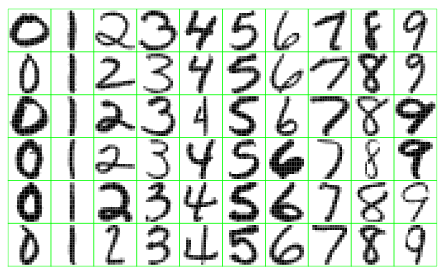
\includegraphics[width=0.66\linewidth]{figures/digits_recognition_v2.png}
	\centering
	\caption[Dígitos escritos a mano.]{Dígitos escritos a mano. Fuente: \citetitle{hastie_elements_2009}
		(\citeyear{hastie_elements_2009}).}
	\label{fig:reconocimiento_digitos}
\end{figure}

\section{Clasificación}

\subsection{Definición}
\label{clasificacion}

La clasificación es una tarea de minería de datos muy popular que consiste en
hallar modelos que describen la o las clases intrínsecas de los datos. La clase
corresponde a un concepto que representa al dato y es una etiqueta categórica,
es decir, un valor discreto de entre un conjunto de valores previamente
conocidos. Estos modelos, también llamados clasificadores, son capaces de
predecir la clase a la que corresponden datos previamente desconocidos. Por
ejemplo, se puede construir un modelo de clasificación para categorizar nuevos
correos electrónicos  de acuerdo a si se trata de correo basura (también
conocido como \comillas{\textit{spam}}) o no. Dicho análisis puede ayudar a
obtener un mayor entendimiento de los datos a alto nivel. Las tareas de
clasificación han sido aplicadas en áreas tales como las de aprendizaje
automático, reconocimiento de patrones o estadística.

En un principio, buena parte de los algoritmos se ejecutaban en memoria, con la
limitación de espacio de almacenamiento que eso conlleva. Investigaciones más
recientes han desarrollado técnicas para escalar los algoritmos de tal manera
que puedan manejar datos de mayor tamaño, alojados en memoria, en disco o
procesados bajo demanda. Las aplicaciones para este tipo de tareas son numerosas
y entre ellas se encuentran las de detectar fraudes o realizar diagnósticos
médicos, entre otras.

La clasificación de datos consta de dos etapas, una de aprendizaje y otra de
clasificación o predicción. Durante la tarea de aprendizaje se construye el
modelo de clasificación  el cual describe un determinado número de clases o
conceptos. También se conoce esta etapa como la de entrenamiento, ya que se
selecciona un subconjunto de los datos, llamado conjunto de entrenamiento, que
consta de instancias o tuplas seleccionadas aleatoriamente y con una o más
etiquetas asociadas. Formalmente, el problema de clasificación puede ser
formulado de la siguiente manera. Se recibe un conjunto etiquetado de
instancias, tupas o ejemplos de la forma $( X, y )$ donde cada tupla es un
vector $X=(x_{1},x_{2},\dots,x_{n})$, siendo cada valor una característica
distintiva, atributo o \textit{feature} de la instancia. El vector $y$ por su
parte toma un valor de entre $n$ clases diferentes.

Este tipo de tareas se engloban dentro del campo de aprendizaje supervisado ya
que para cada instancia la etiqueta es conocida de antemano, y es aprovechada
para guiar o, siguiendo la metáfora, \comillas{supervisar} el aprendizaje del
clasificador. Esta es la diferencia principal contra algoritmos de aprendizaje
no supervisado, en los cuales la etiqueta no es conocida y se deben aplicar
técnicas para salvar esta restricción.

La primera etapa de una clasificación puede ser vista también como el
aprendizaje de una función $y=f(X)$ que pueda predecir la clase $y$ para una
tupla $X$. Por ejemplo, $X$ podría ser un mensaje de correo y la etiqueta $y$ la
decisión de si se trata de un correo basura o no. Desde esta perspectiva
queremos aprender una función que sea capaz de distinguir las clases
subyacentes.  Usualmente, esta asociación es llevada a cabo por algoritmos de
aprendizaje, los cuales internamente usan funciones matemáticas o reglas de
decisión que les permiten procesar los atributos de entrada y generar una salida
acorde. Algunos ejemplos de este tipo de algoritmos son los árboles de decisión,
\textit{naive} bayes, perceptrón, entre otros. Más adelante se retomará sobre
este punto para describir en detalle algunos algoritmos representativos del
campo.

En la segunda etapa el modelo es usado para clasificar y realizar predicciones
sobre datos desconocidos. A este fin, se calcula un valor que refleja la calidad
del clasificador y es denominado \comillas{métrica de evaluación}. Una de ellas
es la exactitud o \textit{accuracy}, pero no es la única.  Durante la etapa de
entrenamiento esta estimación puede ser imprecisa, tomando un valor que tiende a
ser \comillas{optimista} o que da un valor de exactitud mayor al rendimiento
real.  Esto sucede porque el clasificador puede llegar a incorporar anomalías
particulares en el conjunto de datos de entrenamiento, las cuales no tienen que
ver tanto con el dominio de aplicación en el cual se enmarca la tarea, sino más
bien con \comillas{ruido}, datos erróneos o simplemente instancias que no
reflejan correctamente los objetos del mundo real. Este fenómeno es llamado
\comillas{sobreajuste} u \comillas{\textit{overfit}} y se han diseñado técnicas
para reducirlo. Una de ellas consiste en separar de entre los datos de la
colección completa, un subconjunto conocido como \comillas{conjunto de prueba} o
de \textit{testing} que no se usa durante el entrenamiento y a partir del cual
se realizan predicciones y se calculan las métricas de evaluación.

Así pues, la tarea de evaluación es fundamental, ya que es la vía a partir de la
cual se determina qué algoritmos o técnicas son más apropiados que otros para un
problema en particular. Asimismo, provee la información necesaria para corregir
o ajustar los parámetros de los algoritmos y así obtener modelos más robustos.

En definitiva, las etapas de aprendizaje y predicción se aplican
consecutivamente con el objetivo de lograr generar un clasificador capaz de
predecir con éxito las etiquetas de instancias nuevas y a priori desconocidas
por el modelo.

\subsection{Algoritmos}
\label{clasificacion_algoritmos}

Como se mencionó en la sección anterior, una de las etapas de la clasificación
consiste en generar un modelo capaz de clasificar instancias no observadas. En
esta etapa de aprendizaje, se pueden aplicar diversos tipos de algoritmos de
clasificación de acuerdo a la naturaleza de la tarea en particular que se desea
abordar. A continuación, se describen algunos de estos algoritmos en detalle a
fin de ahondar sobre el concepto de clasificación en el aprendizaje automático.
Además, más adelante estos algoritmos serán particularmente relevantes para el
desarrollo del presente trabajo de investigación.

\subsubsection{\textit{Naive} Bayes}

\textit{Naive} Bayes es uno de los algoritmos que pertenecen a la familia de
clasificadores probabilísticos y se destaca por ser computacionalmente simple,
interpretación, y al mismo tiempo brinda un  rendimiento competitivo en
comparación con otros modelos más complejos. Se dice que es un clasificador
estadístico porque se basa en el teorema de Bayes. La idea es computar una
probabilidad para cada una de las clases, basada en los atributos de la
instancia y seleccionar aquella de mayor probabilidad. El término
\comillas{\textit{naive}} es el inglés para el término
\comillas{\textit{ingenuo}} y nace de la presunción que hace el algoritmo de que
los atributos son independientes entre sí, o condicionalmente independientes.
Esta presunción raramente se cumple en los escenarios donde se aplica, pero
contribuye a su simplicidad computacional y a su velocidad durante el
entrenamiento.

Para entender cómo funciona este algoritmo, es bueno abordar primero  el teorema
de Bayes. Formalmente, se define de la siguiente manera:

\begin{equation}
	P(H \mid X) = \frac{P(X \mid H) P(H)}{P(X)}
\end{equation}

En esta ecuación, el vector $X$ es una tupla definida tal como en la sección
anterior y en términos bayesianos representa la \comillas{evidencia}. $P(X)$,
por lo tanto, es la probabilidad de que la tupla contenga los atributos que
efectivamente posee. Por su parte, $H$ es la hipótesis de que la tupla pertenece
a una determinada clase y $P(H)$ su probabilidad. Esta es conocida como
probabilidad \comillas{a priori}. De la misma manera, $P(H|X)$ es la
probabilidad de que la hipótesis $H$ sea cierta bajo la evidencia $X$. A esta se
la llama probabilidad \comillas{a posteriori} con $H$ condicionada por $X$ y es
el valor que se quiere determinar en una tarea de clasificación.  Finalmente,
$P(X|H)$ indica la probabilidad de que la tupla tenga unos atributos
determinados dado que se satisface la hipótesis.

A partir de dicha definición, y de forma similar, se expresa la ecuación de
\textit{Naive} Bayes de la siguiente manera:

\begin{equation}
	P(C_{i} \mid X) = P(X \mid C_{i}) P(C_{i})
\end{equation}

Aquí el término $P(X)$ es descartado porque se asume constante para todas las
clases. La hipótesis $H$ es representada como $C_{i}$ que es un valor de la
tupla $C=(C_{1},C_{2},\dots,C_{q})$, donde $q$ es el número de clases. La
presunción \comillas{ingenua} es aplicada para el cálculo del término $P(X \mid
	C_{i})$ gracias a lo cual se puede definir de la siguiente manera:

\begin{equation}
	P(X \mid C_{i}) = \prod\limits_{k=1}^n{P(x_{k} \mid C_{i})} =
	P(x_{1} \mid C_{i}) \times
	P(x_{2} \mid C_{i}) \times \dots, \times
	P(x_{n} \mid C_{i})
\end{equation}

Finalmente, el modelo seleccionará la clase que maximice el valor de
probabilidad y esa será la salida final del algoritmo.

Como se ha dicho anteriormente, la simplicidad, velocidad computacional y su
competitividad en métricas de exactitud hacen de \textit{Naive} Bayes un
algoritmo destacado en el campo de aprendizaje automático
\cite{wickramasinghe_naive_2020} y ha sido aplicado para problemas diversos,
tales como el de hallar errores en programas de computación
\cite{arar_feature_2017}, predecir enfermedades del corazón
\cite{dulhare_prediction_2018} o detectar ataques en una red de computadoras
\cite{kalutarage_detecting_2015}.


\subsubsection{Árboles de Decisión}

Árboles de decisión es un modelo de clasificación que se destaca por ser de
fácil interpretación e intuitivo para el ser humano. De hecho, se puede generar
una representación gráfica del árbol generado para asistir a la comprensión del
modelo y así entender a más alto nivel cómo se comporta durante una predicción.
En cuanto a su estructura, un árbol de decisión contiene nodos, cada uno
representando un atributo de la colección. Estos nodos se conectan con otros
nodos a partir de enlaces o \comillas{ramas} que representan un valor o un rango
de valores de ese atributo.  Los nodos de menor jerarquía son llamados
\comillas{hojas} y contienen la clase de la predicción, y el nodo de mayor
jerarquía es llamado \comillas{raíz}. Al momento de predecir una instancia
nueva, la clasificación se realiza de la siguiente manera:  se toma la instancia
nueva, la cual no tiene una etiqueta asociada, y los valores de sus atributos
son comparados contra los del árbol, luego se traza un camino desde el nodo raíz
hasta la hoja. Finalmente, la clase que contiene la hoja es seleccionada y será
parte de la predicción resultante.

Los árboles de decisión se generan a partir de un algoritmo de inducción.
Existen varios de estos algoritmos, pero todos son variantes que han sido
diseñadas bajo un mismo principio: construir  el árbol de una manera
\comillas{voraz}\footnote{Se le llama voraz o \textit{greedy} a un algoritmo que
	busca hallar la opción óptima en cada paso y, de esta manera, alcanzar la
	solución general óptima para resolver un problema.  Esto lo diferencia de
	algoritmos como los de \textit{backtracking}, los cuales exploran distintas
	posibilidades y pueden volver al inicio en búsqueda de una mejor solución.},
comenzando desde el nodo raíz (conocido como enfoque \textit{top-down}) y
eligiendo en cada paso el atributo más informativo o que maximice alguna medida
de ganancia de información. Entre estos algoritmos de inducción vale destacar
los siguientes:

\begin{description}

	\item[\acrshort{id3}] Son las siglas de \comillas{\textit{\acrlong{id3}}} y
	      fue desarrollado en 1986 por Ross Quinlan. Consiste en crear un árbol de
	      múltiples vías, buscando para cada nodo el atributo categórico que lance
	      la mayor ganancia de información para las clases categóricas. Los árboles
	      crecen en un tamaño máximo y luego se realiza el paso de poda para mejorar
	      el poder de generalización del modelo sobre datos desconocidos.

	\item[C4.5] Es la evolución del algoritmo \acrshort{id3}. La principal mejora
	      con respecto a su predecesor es que elimina la restricción de que los
	      atributos deban ser categóricos. Esto lo consigue particionando el valor
	      continuo en rangos o en un conjunto de intervalos discretos. A su vez,
	      C4.5 convierte el árbol entrenado en conjuntos de reglas de decisión.

	\item[\acrshort{cart}] Son las siglas de \comillas{\textit{\acrlong{cart}}} y
	      es un algoritmo muy similar al C4.5, pero que soporta clases numéricas, lo
	      cual permite que este algoritmo pueda ser utilizado para resolver
	      problemas de regresión.

\end{description}

Una tarea fundamental en la generación de un árbol es definir un criterio de
división. El objetivo del criterio de división es seleccionar el mejor atributo
en cada paso y existen diversas técnicas para abordar el problema. Una de ellas
es la de \comillas{Ganancia de Información}, usada por el algoritmo
\acrshort{id3}. La técnica de ganancia de información busca seleccionar el
atributo que posee mayor variabilidad o representatividad de los datos y se
sustenta en el cálculo de la entropía o medida de desorden. La idea de fondo es
hallar el atributo que reduzca la entropía esperada. La entropía en el conjunto
de datos $D$ se calcula de la siguiente manera:

\begin{equation}
	Entropia(D) = - \sum_{i=1}^{q} p_{i}\log_{2}(p_{i})
\end{equation}

Nótese que $p_{i}$ corresponde a la probabilidad de que una tupla de $D$
corresponda a la clase $C_{i}$.  A partir de la entropía, se define la ganancia
de información como:

\begin{equation}
	Ganancia(A) = Entropia(D)
	- \sum_{j=1}^{v} \frac{\left\| D_{j} \right\|}{\left\| D \right\|}
	\times Entropia(D_{j})
\end{equation}

Aquí el atributo $A$ divide al conjunto de datos en $v$ particiones, siendo $v$
los valores posibles que toma $A$. $D_{j}$ es el subconjunto de los datos cuyas
tuplas poseen el valor $v$ del atributo $A$, siendo $\left\|D_{j}\right\|$ su
cardinalidad o número de instancias del subconjunto. Al dividir este término por
la cardinalidad del conjunto de datos, se obtiene un valor que representa el
peso de la partición y que es aplicado sobre la entropía esperada. Este proceso
se repite para todos los atributos y, una vez obtenidos los valores de ganancia
para cada uno de ellos, se elige aquel que maximiza la ganancia y finalmente el
atributo seleccionado será el criterio de separación en el nodo.

El algoritmo C4.5 introdujo una mejora en esta técnica llamada \comillas{Razón
	de Ganancia}. La misma busca disminuir uno de los efectos adversos que provoca
la técnica de ganancia de información, esta es, que tiende a favorecer a
atributos con un mayor número de valores posibles. La razón de ganancia, en
primer lugar, reemplaza la fórmula $Entropia(D)$ por la siguiente expresión:

\begin{equation}
	EntropiaRG_{A}(D) = - \sum_{j=1}^{v} \frac{\left\| D_{j} \right\|}{\left\| D \right\|}
	\times \log_{2}(\frac{\left\| D_{j} \right\|}{\left\| D \right\|})
\end{equation}

A partir de allí, el cálculo de la razón de ganancia hace uso de la ganancia y
de la entropía y se formula como:

\begin{equation} \label{eq:gan_c45}
	RazonGanancia(A) = \frac{Ganancia(A)}{EntropiaRG_{A}(D)}
\end{equation}

Finalmente, el atributo de mayor razón de ganancia es seleccionado como criterio
de corte y se continúa el cálculo con los siguientes subnodos.

\subsubsection{Ensambles}
\label{ensambles_intro}
\todo{Figura de ensamble}

Los ensambles son un conjunto de clasificadores cuyas salidas son combinadas
entre sí con el objetivo de realizar mejores predicciones que cualquiera de
ellos individualmente. En pocas palabras, el enfoque de ensambles consiste en
generar $k$ clasificadores llamados \comillas{clasificadores base}, desde un
mismo algoritmo o no, y entrenarlos con distintos subconjuntos de la colección
de entrenamiento original. Dada una tupla nueva, cada clasificador devuelve su
propia predicción, llamada \comillas{voto}, y luego el ensamble combina cada uno
de estos votos siguiendo algún método de combinación elegido, de forma tal de
producir una predicción final óptima.

La aplicación de ensambles en problemas de clasificación nace de la
imposibilidad de generar un único modelo capaz de generalizar lo suficiente como
para lograr un rendimiento perfecto. Ante la presencia de datos ruidosos,
atípicos o erróneos los clasificadores pueden tender a clasificar mejor para un
subconjunto de datos y no tan bien para otros. Este escenario es aprovechado por
el enfoque de ensambles, ya que su éxito tiene correlación directa con la
existencia de \comillas{diversidad} en la clasificación, distinguiendo el
concepto de diversidad como la existencia de variabilidad entre los modelos,
entre hiperparámetros o entre particiones del conjunto de datos. En definitiva
se entiende que, cuanto mayor es esta diversidad, mayor es la probabilidad de
aislar los posibles errores particulares de un modelo, y al suceder esto, el
error terminará siendo filtrado por el ensamble en la clasificación final. En
consecuencia, se espera lograr una disminución del error total de la
clasificación así como también una mayor exactitud en la predicción, comparando
contra la salida individual de cada clasificador base. Sumado a esto, un
enfoque de ensambles abre la posibilidad de distribuir y/o paralelizar el
cómputo de la predicción, pudiendo así mejorar los tiempos de ejecución durante
el entrenamiento.

En suma, existen distintos tipos de ensamble de acuerdo a su construcción y
arquitectura. A continuación se describen tres de ellos: los ensambles de tipo
\comillas{\textit{bagging}}, los de tipo \comillas{\textit{boosting}} y los de
tipo \comillas{\textit{stacked}}.

\begin{description}

	\item[Bagging] Esta es una de las primeras técnicas de ensambles conocidas y
	      fue introducida por
	      \citeauthor{breiman_bagging_1996}\cite{breiman_bagging_1996}. La misma se
	      desarrolla de la siguiente manera: dado un conjunto de entrenamiento $D$
	      con $n$  tuplas, \textit{bagging} genera un número $m$ de nuevos conjuntos
	      de datos de entrenamiento, cada uno con $n$ tuplas. Para esto se toman
	      tuplas del conjunto original de manera aleatoria y con reemplazo, es decir
	      que puede haber tuplas repetidas y otras que no están incluidas en el
	      nuevo conjunto.  Luego a partir de cada conjunto nuevo, se entrena un
	      clasificador $M_{i}$. Cada clasificador puede ser del mismo tipo porque la
	      diversidad está dada por los datos. En la etapa de clasificación, cada
	      modelo $M_{i}$ genera una predicción que cuenta como un voto. El ensamble
	      cuenta los votos y elige la clase con mayor cantidad de votos, siendo esta
	      la decisión final del ensamble.


	\item[Boosting] En la técnica de \textit{boosting} se asigna un peso a cada
	      tupla de entrenamiento y se generan un conjunto de clasificadores, cada
	      uno a partir del anterior. A diferencia del método de \textit{bagging},
	      \textit{boosting} trabaja siempre sobre el mismo conjunto de datos y la
	      variabilidad está dada por los pesos que son asignados. El proceso es el
	      siguiente: para el primer modelo de clasificación, $M_{i}$, los pesos son
	      inicializados en un mismo valor para todas las tuplas. Una vez que se
	      entrena este modelo, los pesos son actualizados de tal manera que el
	      siguiente clasificador $M_{i} + 1$ trate de manera particular a las tuplas
	      mal clasificadas por $M_{i}$. De ese modo se busca llegar a una
	      clasificación correcta en las sucesivas iteraciones.  Finalmente, el
	      modelo de ensamble combina los votos de cada clasificador individual. Cabe
	      notar que el peso de cada voto también es ponderado de acuerdo al
	      rendimiento del clasificador base.


	\item[Stacking] La técnica de \textit{stacking} fue desarrollada por
	      \citeauthor{wolpert_stacked_1992}\cite{wolpert_stacked_1992} y consiste en
	      entrenar un nuevo clasificador de acuerdo a las predicciones realizadas
	      por otros modelos, tomando la salida de estos modelos como entrada, de tal
	      manera de lograr hallar una combinación que produzca una mejor predicción.
	      Este tipo de ensambles puede ser visto como un conjunto de capas. La
	      primera capa consta de un ensamble de clasificadores que aprenden a partir
	      de los datos de entrenamiento. Esta capa no necesariamente usa
	      clasificadores del mismo tipo, mismos hiperparámetros o particiones de la
	      colección iguales, quedando estos detalles a cargo de quien diseña esta
	      capa. La siguiente capa es el clasificador individual, o
	      meta-clasificador, que se alimenta de las salidas de los clasificadores de
	      la capa inferior y realiza el aprendizaje a partir de las clases
	      producidas por estas salidas y las clases reales.

\end{description}

Una de las tareas a tener en cuenta durante el entrenamiento de un ensamble es
la de combinar las salidas de cada modelo en una salida final. La estrategia más
común y simple es la de votación por mayoría, la cual normalmente es aplicada
por los métodos de \textit{bagging}. No obstante, existen múltiples métodos de
combinar los votos, e incluso no siempre un ensamble de tipo \textit{bagging}
debe aplicar esta estrategia. Por ejemplo, algunos clasificadores pueden decidir
producir una salida solo en el caso de que más de la mitad de ellos coincidan, o
incluso ser más restrictivos y obligar a que la coincidencia sea total. El
enfoque de \textit{boosting} por su parte, pondera al voto de acuerdo a los
pesos que calcula, dando predominio a determinadas instancias.  También se suele
dar un mayor peso a determinados clasificadores por sobre otros. Este tipo de
métodos se los denomina \comillas{votación por mayoría ponderada} y pueden
llevar a un rendimiento superior si es aplicada en el escenario adecuado.

\subsection{Evaluación}
\label{evaluacion_intro}

Llevar a cabo evaluaciones de rendimiento sobre los modelos es un aspecto
importante del aprendizaje automático, ya que nos permite conocer en qué medida
un algoritmo es superior a otro para resolver una tarea. Particularmente, la
tarea de clasificación es un desafío que se presenta en un contexto cambiante y
evolutivo, donde nuevas herramientas surgen y se actualizan constantemente.
Incluso la composición y estructura de los modelos de clasificación varía según
la familia de algoritmos aplicados, y es esperable que los conceptos extraídos
de un modelo de tipo árbol tengan particularidades que lo diferencien de modelos
de redes neuronales o modelos probabilísticos. Y del mismo modo, es esperable
que alguno de estos modelos tenga un mejor rendimiento que otro en un
determinado escenario, o incluso que sea mejor que un modelo generado por el
mismo algoritmo pero con distintos hiperparámetros. La tarea de evaluación es
la que permite detectar estas particularidades y sacar provecho de los
algoritmos para obtener aún mejores modelos.

A su vez, es importante estudiar las métricas de evaluación existentes y llevar
adelante estrategias que nos permitan obtener medidas de evaluación confiables y
que no hayan sido sesgadas por los datos que se usaron durante el entrenamiento.
Y del mismo modo, entender los factores que provocaron un valor de métrica puede
ser el paso inicial para hallar mejoras al modelo que optimizan su capacidad de
predicción en el futuro.

Por consiguiente, a continuación se estudian algunas de las estrategias llevadas
a cabo durante la evaluación para evitar sesgos, así como también las métricas
que se calculan durante este proceso.

\subsubsection{Métricas}
\label{evaluacion_metricas}

Las métricas de evaluación se usan para conocer la habilidad predictiva de un
modelo de clasificación. Se van a describir aquí las métricas más conocidas del
campo y que proveen, a su vez, un primer vistazo de lo que serán las métricas
usadas para evaluar algoritmos para datos multi-etiquetados en las futuras
secciones del escrito.

Antes de comenzar es importante aclarar algunos términos que serán usados para
definir las métricas. Se entiende como \comillas{ejemplos positivos} a aquellas
instancias cuya etiqueta pertenece a la clase de interés en el problema de
estudio y \comillas{ejemplos negativos} como aquellas que no pertenecen a dicha
clase. Al mismo tiempo, se derivan cuatro conceptos que estarán presentes en las
fórmulas para calcular las métricas, los cuales son:

\begin{description}

	\item[\acrfull{vp}] Son los ejemplos positivos que fueron correctamente
	      clasificados como positivos.

	\item[\acrfull{vn}] Son los ejemplos negativos que fueron correctamente
	      clasificados como negativos.

	\item[\acrfull{fp}] Son los ejemplos negativos que fueron incorrectamente
	      clasificados como positivos.

	\item[\acrfull{fn}] Son los ejemplos positivos que fueron incorrectamente
	      clasificados como negativos.

\end{description}

Una vez obtenidos estos conceptos se pueden calcular una serie de métricas a
partir de ellos. Estas métricas son:

\paragraph{Exactitud}
\label{evaluacion_metricas_exactitud}

La exactitud o \textit{accuracy} es la proporción de ejemplos correctamente
clasificados sobre el número total de instancias y a mayor el valor de exactitud
mejor es el rendimiento del clasificador. Se define  como:

\begin{equation}
	exactitud = \frac{\acrshort{vp} + \acrshort{vn}}{\acrshort{vp} +
		\acrshort{vn} + \acrshort{fp} + \acrshort{fn}}
\end{equation}

\paragraph{Tasa de Error}

A la inversa de la exactitud, la tasa de error es la proporción de ejemplos
incorrectamente clasificados sobre el número total de instancias y a menor el
valor de la tasa de error mejor es el rendimiento del clasificador. Se define
como:

\begin{equation}
	tasaError = \frac{\acrshort{fp} + \acrshort{fn}}{\acrshort{vp} +
		\acrshort{vn} + \acrshort{fp} + \acrshort{fn}}
\end{equation}

\paragraph{Precisión}

La precisión es la proporción de ejemplos que fueron clasificados como positivos
y que efectivamente lo son. Mayor es el valor de precisión mejor es el
rendimiento del clasificador. Se dice que es una medida de exactitud y se define
como:

\begin{equation}
	precision = \frac{\acrshort{vp}}{\acrshort{vp} + \acrshort{fp}}
\end{equation}

\paragraph{Exhaustividad}

La exhaustividad o \textit{recall} es la proporción de ejemplos positivos que
fueron clasificados como positivos. Mayor es el valor de exhaustividad mejor es
el rendimiento del clasificador. Se dice que es una medida de completitud y se
define como:

\begin{equation}
	exhaustividad = \frac{\acrshort{vp}}{\acrshort{vp} + \acrshort{fn}}
\end{equation}

\paragraph{Medida-F1}

La medida-F1 o \textit{f1-score} es una medida que integra las métricas de
precisión y exhaustividad tomando la media harmónica entre ambas. Mayor el valor
de esta medida, mejor es el rendimiento del clasificador. Se define como:

\begin{equation}
	medidaF1 = \frac{2 \times precision \times exhaustividad}
	{precision + exhaustividad}
\end{equation}

Por otro lado, existen métricas para evaluar la eficiencia del clasificador en
términos de velocidad y consumo de memoria. Estas métricas cobran especial
importancia en ambientes de flujos continuos de datos, donde el volumen de datos
es grande, la velocidad en la que arriban es alta y los recursos escasean. A
continuación se añade una breve descripción de ambas.

\paragraph{Velocidad}

La velocidad se refiere al costo computacional de generar el modelo y realizar
predicciones, en general se deja fuera del cálculo los tiempos invertidos en
cargar la colección en memoria, realizar tareas de normalización y
preprocesamiento sobre los datos y otras etapas de la clasificación. A menor el
tiempo de ejecución, mejor es el rendimiento del algoritmo.

\paragraph{Consumo de Memoria}

El consumo de memoria es un indicador de los requerimientos de memoria
aproximados para almacenar el modelo, así como también un indicador de resguardo
para estimar el posible consumo de memoria durante la ejecución y asegurarse que
el algoritmo se mantiene en actividad. A menor el consumo de memoria, mayor es
la eficiencia del modelo.

\subsubsection{Estrategias}
\label{evaluacion_estrategias}

Una vez que se define la métrica o el conjunto de métricas apropiadas para
medir el rendimiento de los clasificadores, el siguiente desafío es seguir un
procedimiento de pruebas capaz de lograr resultados de evaluación que puedan ser
generalizables a conjunto de datos aún no observados. Las técnicas de
\comillas{\textit{Holdout}} y \comillas{Validación Cruzada} son dos de las
técnicas más populares para evaluar la habilidad predictiva de los
clasificadores y se describen a continuación.


\paragraph{\textit{Holdout}}

En este método un conjunto de instancias es separado de la colección y se
reserva para evaluar el rendimiento del clasificador.  Este subconjunto es
distinto del conjunto de datos de entrenamiento usado para generar el modelo y
es llamado \comillas{conjunto de pruebas o \textit{testing}}. Una vez entrenado,
el clasificador recibe las instancias del conjunto de pruebas, pero sin incluir
las etiquetas. La salida del clasificador son las etiquetas de cada instancia.
Finalmente, las etiquetas producidas durante la predicción y las etiquetas
reales de cada instancia se combinan y se calculan las métricas de evaluación.
Esta técnica se basa en la idea de que, separando los datos que se usan durante
el entrenamiento de aquellos usados durante la predicción, se logra una
independencia en los datos que derivará en un mayor grado de generalización en
el modelo.

Por contrapartida, el enfoque de \textit{Holdout} tiene la limitación de que
para lograr generalizar requiere de un número de instancias considerable.
\todo{citar fuente} Esta idea proviene del hecho de que muy pocos datos en el
conjunto de entrenamiento puede derivar en predicciones pobres, pero, por el
contrario, muy pocos datos en el conjunto de pruebas tampoco es recomendable, ya
que podría resultar en medidas de rendimiento poco fiables. A esto se suma una
de las dificultades más comunes en el área de aprendizaje automático: la falta
de disponibilidad de colecciones grandes de datos del mundo real.

Por estas razones, ha tomado peso el uso de técnicas de muestreos de datos para
reutilizar instancias de entrenamiento y de prueba. Una de ellas es la de
validación cruzada.

\paragraph{Validación Cruzada de K iteraciones}

La técnica de validación cruzada, más conocida por el inglés \textit{k-fold
	cross-validation}, consiste en particionar el conjunto de datos en $k$
subconjuntos de manera aleatoria y en la forma $\{d_{1}, d_{2},  \dots, d_{k}
	\}$, siendo cada uno de los subconjuntos mutuamente excluyentes entre sí y de
igual o similar tamaño. El proceso itera sobre cada uno de los subconjuntos para
generar $k$ modelos. En la primera iteración $i$, se separa el subconjunto
$d_{i}$ y se entrena el modelo con los restantes subconjuntos para luego medir
el rendimiento con él. En la segunda iteración, se repite este procedimiento
pero usando como pruebas al subconjunto $d_{i+1}$, y así en cada iteración. Así
pues, cada subconjunto es usado una vez para probar el modelo. Finalmente, se
toman los $k$ modelos generados y se promedian las métricas.

De esta técnica derivan otras similares como \comillas{\textit{leave-one-out}}
en donde cada subconjunto es conformado por $n-1$ instancias, siendo $n$ el
tamaño de la colección, dejando un elemento fuera del subconjunto y que será
usado para validar el modelo. El proceso se repite $n$ veces y se combinan los
modelos tal como en el método de validación cruzada.

Otra técnica similar es la de \comillas{Validación Cruzada Estratificada}, la
cual consiste en generar subconjuntos de entrenamiento y pruebas que respeten la
representación de clases existentes en la colección inicial. Por ejemplo, si una
de las clases del problema aparece en el $25\%$ de las instancias, este método
asegura que al generar las particiones esa clase continuará siendo representada
por el $25\%$ de las tuplas. Esta técnica puede ser útil para problemas donde
existe una diversidad que es necesario reflejar en las particiones para obtener
medidas precisas.

En general, los investigadores recomiendan usar validación cruzada con $k=10$ ya
que se suelen conseguir estimaciones menos sesgadas sin incurrir en costos
computacionales demasiado altos.



\backmatter

%%%% GLOSARIO
\printglossary[type=\acronymtype]
\cleardoublepage

%%%% BIBLIOGRAFIA
% textidote: ignore begin
\printbibliography
% textidote: ignore end

\end{document}
